\documentclass[11pt]{report}
% packages
% Fran Burstall's Bath thesis package
\usepackage{baththesis}
\usepackage{amssymb} %for Blackboard bold etc \usepackage{graphicx} %for including eps graphics % front matter
\usepackage[pdftex]{graphicx} % To include pictures
\usepackage{caption}
\usepackage{subcaption} % To use subfigures with subcaptions
\usepackage{url}
\usepackage{amsmath} % Equations
\usepackage{txfonts}
\setlength{\parskip}{0.9em} %Paragraph spacing
\usepackage{pgfgantt}
\usepackage{cite}
\usepackage{csquotes}
\usepackage[ruled]{algorithm2e} % Algorithms 
\renewcommand*{\mkcitation}[1]{ #1}
\usepackage{listings} % For C++ code
\lstset{language=C++,
                basicstyle=\scriptsize,
                keywordstyle=\color{blue}\ttfamily,
                stringstyle=\color{red}\ttfamily,
                commentstyle=\color{green}\ttfamily,
                morecomment=[l][\color{magenta}]{\#},
                showstringspaces=false
}

\newcommand{\phim}{\mathbf{\phi}}
\newcommand{\X}{\mathbf{X}}
\newcommand{\x}{\mathbf{x}}
\newcommand{\Y}{\mathbf{Y}}
\newcommand{\y}{\mathbf{y}}
\newcommand{\w}{\mathbf{w}}
\newcommand{\Z}{\mathbf{Z}}
\newcommand{\z}{\mathbf{z}}
\newcommand{\h}{\mathbf{h}}
\newcommand{\dd}{\: \mathrm{d}}
\newcommand{\B}{\mathbf{B}}
\newcommand{\F}{\mathbf{F}}
\newcommand{\bb}{\mathbf{b}}
\newcommand{\vect}[1]{\mathbf{#1}}
\newcommand{\Maya}{Maya\textsuperscript\textregistered}
\newcommand{\Matlab}{Matlab\textsuperscript\textregistered}

%\usepackage[hidelinks]{hyperref} % Adds references links without color
\usepackage{hyperref} % Adds references links with color
\usepackage{xcolor}
\hypersetup{
    colorlinks,
    linkcolor={red!50!black},
    citecolor={blue!50!black},
    urlcolor={blue!80!black}
}

\DeclareMathOperator*{\argmin}{arg\,min}
\DeclareMathOperator*{\argmax}{arg\,max}

\title{Performance-driven Facial Animation} \author{Garoe Dorta-Perez, Ieva Kazlauskaite, Richard Shaw}
%\degree{Doctor of Philosophy}
\unit{ CM50247 - Visual Effects }
\department{} 
\degreemonthyear{May 2015}
\norestrictions

\begin{document}
\maketitle

\chapter{Introduction}
\label{ch:intro}
\begin{center}
\textquote[~\cite{Attenborough:1998}]{\textit{Birds are the most accomplished aeronauts the world has ever seen. They fly high and low, at great speed, and very slowly. And always with extraordinary precision and control}.}
\end{center}

A talented painter or sculptor is able to imagine and reproduce the subtle details of a human face. Hours of training and endless manual adjustments are required before an arbitrary shape resembles a facial expression. Furthermore, a human eye is trained to notice subtle changes in the expression of another human being, which also applies to animated humans, thus even the smallest discrepancies in an animated model are easily detected. Though artists are able to produce good quality and appealing results, the limitations in budget and time so prominent in the entertainment industry motivate the development of more automated, faster and cheaper models.

The naive approach that allows for faster performance is the keyframe animation; though it is based on manual input, keyframe animation requires fewer frames as the intermediate expressions are interpolated over. However, this approach is still very laborious and time consuming. With the emergence of sophisticated systems and software for motion capture, development of methods for performance-driven animation has received significant attention from both the industry as well as the academia.



%-----------------------------------------------------------------------
\chapter{Previous Work}
\label{sec:previous}

\section{Data Capture}



%-----------------------------------------------------------------------
\section{Sparse Reconstruction}


%-----------------------------------------------------------------------
\section{Facial Animation} \label{sec:prfacialanimation}


% INTRO TO JOSHI 2013 PAPER.

The first attempts at using performance-driven facial animation in academia date back to late $20^{th}$ century while in industry it was first used for guidance rather than production, for instance the facial motion of Gollum in the \textit{Lord of the Rings} was based on the motion capture data of the performance of the role actor Andy Serkis~\cite{Pighin:2002}. Another notable example is the pipeline used in the making of \textit{the Polar Express}; the motion capture data was used to construct a multilayer facial rig that was used by an artist to create the final facial animation~\cite{Bennett:2005}. Though many other examples exist, often the exact technology and methods used in production are not disclosed. % ADD MORE INDUSTRY EXAMPLES FROM DIGITAL EMILY PAPER.

In the last two decades, nearly two hundred academic papers that include words \textit{face}, \textit{animation} and \textit{motion capture} were published in computer graphics and vision journals ~\cite{Scopus}. The increase in the quality of the results is explained by the advancements in both the capturing technology and the computational methods. We shall concentrate on the latter; for a brief discussion of the capturing methods see Sec.~\ref{sec:datacapture}. 

The work of Guenter et al. provides the first detailed and unified system for capturing and reconstructing facial performance~\cite{Guenter:1998}. Their work is mostly focused on motion tracking and production of labelled three-dimensional motion of the dots on the actor's face. Once a sequence of  moving dots is acquired, the author's face is scanned to obtain a polygonal mesh that corresponds to the geometry of the face. The motion of the sparse dots is described in terms of offsets from the neutral position. Then the vertices in the mesh are moved by calculating a linear combination of the offsets of the nearest dots, i.e. in each frame a weighted sum of the change in the dot position is calculated and added to the neutral position of the given vertex. The weights are chosen to be zero everywhere except in the one-ring neighbourhood where the weights depend on the distance of the vertex to the dots; the weights must sum to one. An additional stationary ring of dots is added on the edge of the face to ensure there is no motion outside the face. The algorithm suffers from noise introduced during in the tracking, the reconstruction and the three-dimensional scanning. Moreover, the choice of the nearest dots for each vertex in the mesh is not trivial due to the irregular distribution of the tracked dots. The method that assigns the blends has a number of manually adjusted parameters and does not guarantee to find the best set of reference dots. Additionally, the areas around the eyes and lips require a special treatment; the dots above and below the problematic areas are marked and are not allowed to be blended. The authors point out that a number of artefacts are visible in the resulting animation; some of these flaws are attributed to the poor quality of the facial scan, the fact that the reconstruction method is not robust to jitter and incorrect placement of the tracked data.

At around the same time Pinghin et al. proposed a method for synthesizing facial expressions form photographs~\cite{Pighin:1998}. The authors concentrate their attention on the capture and reconstruction part of the process. First, a three-dimensional model of the face pulling a number of different expressions is constructed, then the animation is created by morphing these meshes and producing the intermediate motion. The meshes are topologically consistent and the features are marked manually, resulting in matching feature sets. Then linear interpolation between corresponding vertices in the different meshes is used to get a smooth morphing. Compared to the method proposed by Guenter et al., the approach of Pinghin et al. puts more emphasis on the capture, reconstruction, and creation of good quality meshes for different expressions resulting in an almost trivial animation production process.

Noh and Neumann addressed the problem of having to create a new model for a new animation by exploiting an existing database of high quality animations~\cite{Noh:2001}. Given a new target model, dense correspondence between the source model from the database and the target is estimated using a set of manually selected matching points. The volume morphing is performed using a weighted linear combination of Radial Basis Functions (RBF). However, some manual input is required when matching the features; for this authors employ a set of heuristic rules. Then a cylindrical projection is used to transfer the vertices from the source onto the target model, thus the source vertices are embedded in the target surface. The animation is created by applying the adjusted target motion vector to the source. The adjustments involve scaling, and change of direction according to the curvature of the source surface. Moreover, if the two models have very different geometries, then small neighbourhoods are used to determine the local changes that were imposed during the morphing of the source surface. As in most facial models, special attention is paid to the area around the mouth; the edges of the lips in the two models are aligned, and the motion transformations take into account the motion of both lips to ensure that the duplicated vertices move consistently. The presented approach has a number of limitations; the model requires manual matching, the eyelids, the teeth and the tongue are not incorporated in the model, and it is only able to reproduce the motion of the source model and cannot produce novel movements. 

Building on previous work on synthesis of facial expressions, by Joshi et al. address the problem of automating the creation of blendshapes~\cite{Joshi:2003}. The proposed method segments the face into characteristic parts that can then be modified independently to make a desired expression thus simplifying the process of creating new blendshapes. The authors argue that one of the advantages of controlling small regions is the increased number of expressions that may be produced using the blendshapes. Each frame in the keyframe animation is produced by calculating the linear combination of blendshapes in each region. A linear elasticity model is used to deform the surfaces. A related method,  proposed by Pyun et al. generates a new facial expression by combining emotional and verbal key expressions~\cite{Pyun:2003}. The main limitation of this model is that a set of key expressions have to be designed by an artist. 

In some situations the sets of blendshapes is only available for the target model. Choe and Ko propose a method that constructs a set of source key shapes given the target key shapes~\cite{Choe:2005}. First, a mapping between the source and the target coordinate systems is constructed. Then the method iteratively refines the set of shapes using the captured source data. The authors build on their previous work, and use a muscle actuation basis as opposed to the surface-based key shapes. The elements in the actuation basis are linearly independent and they span the corresponding space, forming a complete basis for the facial expressions~\cite{Choe:2001}. However, the actuation basis is much harder to construct in comparison to the surface-based  set of shapes and the relation between the motion of facial muscles and the resulting motion of the facial tissue is not straight-forward.

Vlasic et al. proposed an novel approach to facial animation that is based on a multilinear model~\cite{Vlasic:2005}. The work offers an alternative approach to blendshape models; it involves creating a large dataset that encodes various features, for instance the identities, expressions and location of vertices. Each dimension of the data tensor corresponds to a unique feature, and due to the independence of modes, each feature may be varied without affecting the others. Such model can be extended to include an arbitrary number of features, and may be used for motion retargeting or actor replacement, when a database of three-dimensional scans is available. Moreover, the probabilistic interpretation of the model is related to probabilistic principal component analysis, and is able to deal with missing data. 

A number of dimensionality reduction techniques have been used to produce facial animation; for example Blanz and Vetter apply principal component analysis (PCA) to create a controllable low dimensional model~\cite{Blanz:1999}. Deng et al. use PCA to find a correspondence between the motion capture data are the manually tuned blendshape model~\cite{Deng:2006}. An extension to nonlinear dimensionality reduction techniques was presented by Wang et al.~\cite{Wang:2004}. The proposed method separates the time-varying facial expressions and the individual style associated with the performer. Then the locally linear embedding (LLE) framework is used to find a nonlinear mapping from the high dimensional space onto a low dimensional manifold. The LLE method is based on an assumption that small neighbourhoods around each data point may be treated as linear patches. Using the resulting generative model, new expressions or an animation may be produced by sampling from the low dimensional manifold.
Dimensionality reduction is used when no blendshape model is available, or when different features of the data need to be extracted.

Most of the previously described methods are unable to capture and reproduce the fine details on the actor's face; Bicket et al. introduced a method that is able to create detailed wrinkles on the target model~\cite{Bickel:2007}. The approach is based on decomposition of the model into coarse features from the motion capture sequence, and fine features from the accompanying video. The novel part of their method relies on capturing, analysing and reproducing the wrinkled surface. In the tracking stage, uniform B-Splines are fitted to each fold of the skin. Then the shape of each fold is estimated by exploiting the self-shadowing effect, and finding the gradient that describes the shape of each fold. Moreover, the coupling behaviour is modelled separately. New wrinkles are synthesised by minimising the associated non-linear shell energy; the geometrical model, proposed by Grinspun et al. estimates the local curvature of a surface, and is able to capture the behaviour of thin flexible structures~\cite{Grinspun:2003}. The facial model with detailed wrinkles relies on the quality of the captured data; in particular, the areas that are prone to small-scale deformations have to be painted in a way that minimises diffuse reflection.

One of the most successful attempts to produce a photo-realistic facial animation is known as the Digital Emily project~\cite{Alexander:2009}. The proposed pipeline involves collecting high resolution data, building a detailed facial rig of the actor's face, producing an animation from the video data, and reproducing the high quality results. The blendshape model was created using approximately $30$ three-dimensional scans; since each scan contained more than one discrete shape, a splitting algorithm had to be used to obtain a larger set of controllable shapes. Additional subtle effects, such as the motion of the deformation of the eyelid when the eyes are closed were included to increase the realism of the results. The animation is produced using a number of example poses, and generating predictions for the required pose of the digital model. The entire production process is very time consuming and requires manual input from skilful artists and animators. The authors do not provide a detailed description of the method but their controllable facial rig is publicly available.

One recent development was proposed by Bouaziz et al., who develop a method for real-time facial animation~\cite{Bouaziz:2013}. The new method does not rely on the construction of a three-dimensional expression model  associated with the actor prior to the face animation stage. The presented method uses a consumer-level device that captures both the intensity and the depth (RGB-D cameras); previous research by Baltru\v{s}aitis et al. indicates that the use of multimodal data improves the quality of feature tracking~\cite{Baltrusaitis:2012}. To achieve real-time results, Bouaziz et al. use a template blendshape model that is constantly updated to better match the face of the performer. This update includes two steps. Firstly, PCA is used to construct a low dimensional representation of a large set of different facial meshes, then any new face is constructed by merging the average face with a linear combination of the orthonormal basis vectors produced by PCA. Secondly, surface deformation field is used to further refine the blendshape model. Then the tracking, retargeting and production of an animation is performed in parallel with the optimisation algorithm that aims to personalise the blendshape model. 

Concurrently, Li et al. combined blendshape models with facial tracking to animate a target character face~\cite{Li:2013}. The authors employ per frame correctives to achieve run time shape correction. The data is captured using RGB-D cameras. The initial state of this method consists of capturing a three-dimensional model of an actor's face, and PCA  and a large database of captured facial data is used to construct a generic face. A blendshape model is constructed using the deformation transfer algorithm, proposed by Sumner and Popovi\'{c}~\cite{Sumner:2004}. Then the motion is produced using blendshapes, and it is refined using an orthogonal adaptive basis. This basis is constructed using PCA, and it contains the initial blendshapes as well as a set of corrective shapes; these additional basis elements correspond to expressions that are not contained in the original shape set. The corrective shapes capture the fine-scale details. Due to the non-linear nature of the resulting blendshape model, Laplacian deformations are used to align the tracked data to the three-dimensional model. Then the expectation-maximisation algorithm is used in the adaptive PCA space to iterative improve the space of the corrective shapes. Specifically, given a number of sufficiently diverse input samples and the initial guess of the corrective space, the algorithm estimates the coefficients of the corrective space. Then, the algorithm finds the model that best explains the samples given the corrective coefficients. After each two cycles of the algorithm, the newly acquired corrective space is orthonormalised, and used to decrease the error during the tracking. This method is capable of producing appealing visual results in real-time. However, it requires a scan of the actors face, and the corrective shapes are not directly used during the retargeting.

A different direction was chosen by Garrido et al., who aim to reconstruct high quality three-dimensional models using data only from a monocular video~\cite{Garrido:2013}. The method relies on a pre-designed blendshape model, and uses optical flow to produce three-dimensional motion. Meanwhile, Xu et al. improved the retargeting of facial animation from an actor onto a digital model~\cite{Xu:2014}. The authors use a multi-scale approach, where a targeted optimisation algorithm is used to achieve best results at the course and the fine scale. Moreover, the proposed method provides the user with a set of control tools that are used to alter the automatically produced results. This blendshape model produces high-quality visual results but it still requires significant input from the user.

%there exist a trade-off between the effort 

%-----------------------------------------------------------------------
\section{Skin Rendering}

Rendering realistic skin is a challenging task.
As social beings we interact with interact with other individuals on a daily basis, which has made human perception quite sensitive to skin appearance, even more so with human faces.
Skin is composed of several layers with different properties, to accurately simulate skin the light transport between this layers has to be simulated.
The full effect of light scattering between two points on the surface can be modelled using a Bidirectional Surface-Scattering Distribution Function (BSSRDF).

Weyrich et al~\cite{Weyrich2006} proposed a two-layer model for skin rendering, the outer layer simulates the air-oil interface and the inner layer models the subsurface scattering in the skin.
The authors considered the scattering to be homogeneous, with this assumption they measured the skin BRDF of several subjects in a light dome, while the scattering was sampled at three points in the face with a custom made sensor.
The BRDF data was fitted to a Blinn-Phong and a Torrance-Sparrow isotropic models, and the scattering was fitted with a single transport coefficient.
Donner et al~\cite{Donner2008} also proposed a two-layer model, however the authors allow for the layers to be heterogeneous.
With this addition they are able to introduce the effects of haemoglobin, veins and tattoos.
Emotional induced haemoglobin variations have also been explored ~\cite{Jimenez2010}.
The authors measured the haemoglobin distributions of several subjects in different poses, then a linear combination of the captured data would determine the final haemoglobin distribution for a new sequence.
Recently, Iglesias et al~\cite{Iglesias2015} introduced a five-layer model to handle skin ageing.
Haemoglobin, collagen and fat changes with age are modelled using the different layers.

Normal maps are use to alter the normals of the scene objects during rendering.
This technique is used to add geometric detail to an object at rendering time without actually changing the geometry.
%The error introduced with this approach is shown in Figure \ref{fig:normal_map}, a ray $r_1$ hist the geometry at point $p$ and the normal $n_p$ is used for shading, while if we had the based geometry the hitting point would be $p'$ and the normal $n'$.
Normal maps for skin rendering are usually captured using expensive light domes with a number of synchronized cameras ~\cite{Graham2013, Weyrich2006}. 

Another technique to increase the quality of a face render is to scale the resolution of the textures being used.
According to cite{Tian2011} super-resolution techniques can be classified into four classes: \textit{frequency-domain}-based,	\textit{interpolation}-based, \textit{regularization}-based and \textit{learning }-based.

\textit{Frequency-domain}-based super-resolution methods started with the seminal work of ~\cite{Tsai:1984}, the authors transformed the image using the discrete Fourier transform, where it is possible to formulate a system of equations relating the discrete and the continuous Fourier transform coefficients.
The system is solved, the new coefficients are apply in the Fourier domain and a new image of higher resolution is retrieved by performing the inverse transformation.
More recently, extensions that include denoising stages \cite{Chappalli:2005} or error handling for registration and blur identification \cite{Ji:2009} has been proposed.

\textit{Interpolation}-based approaches used the fact that if we have several low-resolution images of a scene, each of them provides an amount of additional information about the scene.
This technique projects all the low-resolution images into the hight resolution space and fuses the data maximizing the quality.
Bose et al.~\cite{Bose:2006} proposed a fusing technique using the moving least square (MLS) method, the authors estimated the pixel value as a polynomial approximation of the pixel neighbourhood with adaptive polynomial order for each pixel.
Takeda et al.~\cite{Takeda:2007} proposed a method to generalize this and other problems such as denoising or interpolation into a generalized kernel regression problem.

\textit{Regularization}-based methods tackle the problem from a probabilistic viewpoint.
An estimation using the maximum likelihood (ML) of the high-resolution image $\mathbf{X}^{ML}$ was proposed by Tom et al.~\cite{Tom:1995}, such that

\begin{equation}
\mathbf{X}^{ML} = \underset{\mathbf{X}}{\argmax} P(\mathbf{Y} | \mathbf{X}),
\end{equation} 

where $\mathbf{Y}$ the unknown high-resolution image and $\mathbf{X}$ is the low resolution image.
Extensions using maximum a posterior (MAP) with Markov random fields ~\cite{Humblot:2006} and Markov Chain Monte Carlo methods ~\cite{Tian:2010} have been researched.

In the \textit{learning}-based area, Wie et al.~\cite{Wei:2000} proposed a technique to synthesized new textures based on a sample image and a random noise.
The main idea of the authors work was to maximize the local similarity when choosing a new pixel in the synthesized texture image, based on the already built neighbourhood in the new image.
Ashikhmin et al.~\cite{Ashikhmin2001} presented a method to generate new textures using a goal image by greedily extending existing patches whenever possible.
Hertzmann et al.~\cite{Hertzmann2001} combined and extended Ashikhmin et al.~\cite{Ashikhmin2001} and Wie et al.~\cite{Wei:2000} methods by adding a second example image and using more complex distance metric to choose the next synthesized pixel.
Graham et al.~\cite{Graham2013} applied Hertzmann et al.~\cite{Hertzmann2001} example-based filter to generate bump maps with increased quality for skin rendering.
An alternative approach using a dictionary of samples was presented by Jianchao et al.~\cite{Jianchao2010}.
This method is restricted to generating super-resolution images, however, the previous methods support a wide variety of filter effects.
For an in depth analysis of super-resolution techniques, we refer the readers to Tian et al.~\cite{Tian2011} survey.

%\begin{figure}[htbp!]
%\centering
%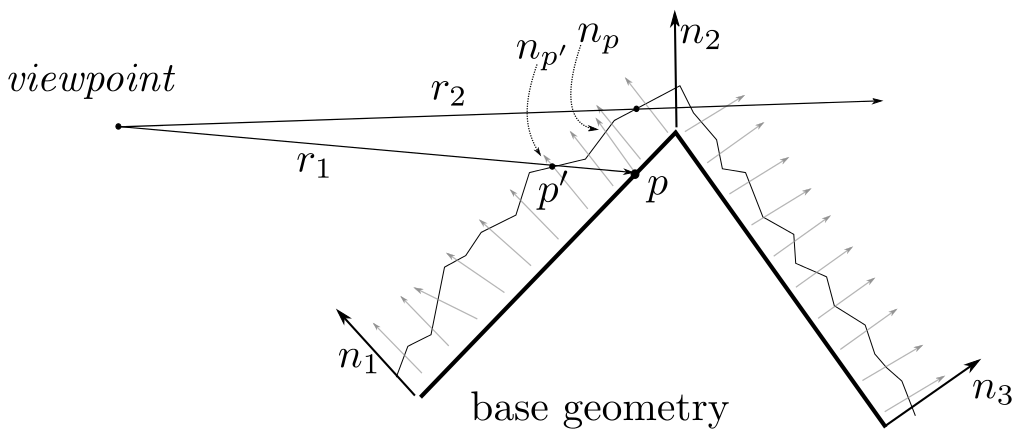
\includegraphics[width=0.7\textwidth]{img/normal_map}
%	\caption{ Using normal maps to simplify a given geometry, image taken from \cite{ganovelli2014}.}
%	\label{fig:normal_map}
%\end{figure}



%-----------------------------------------------------------------------
\chapter{Methodology}
\label{sec:methods}

\section{Pipeline}

The proposed pipeline is shown below...

\section{Data Capture} \label{sec:datacapture}

Two DSLR cameras were positioned in a stereo configuration to capture the actor's facial performance, as shown in Figure \ref{fig:setup1}. The facial performance was recorded on video with a resolution of $640 \times 480$ at 60fps, and the cameras were roughly synchronised by aligning the two separate audio signals. Fixing the cameras close to one another at approximately 10cm separation, and about 1m distance from the subject, meant that the images from both views would be quite similar, allowing for easier feature matching across the two images. However, the camera spacing was sufficiently large to enable both sides of the face to be in view, and to allow for triangulation of points on the face; a good rule of thumb is for the cameras and subject to subtend an angle of at least 5 degrees. 

\begin{figure}[htbp!]
\centering
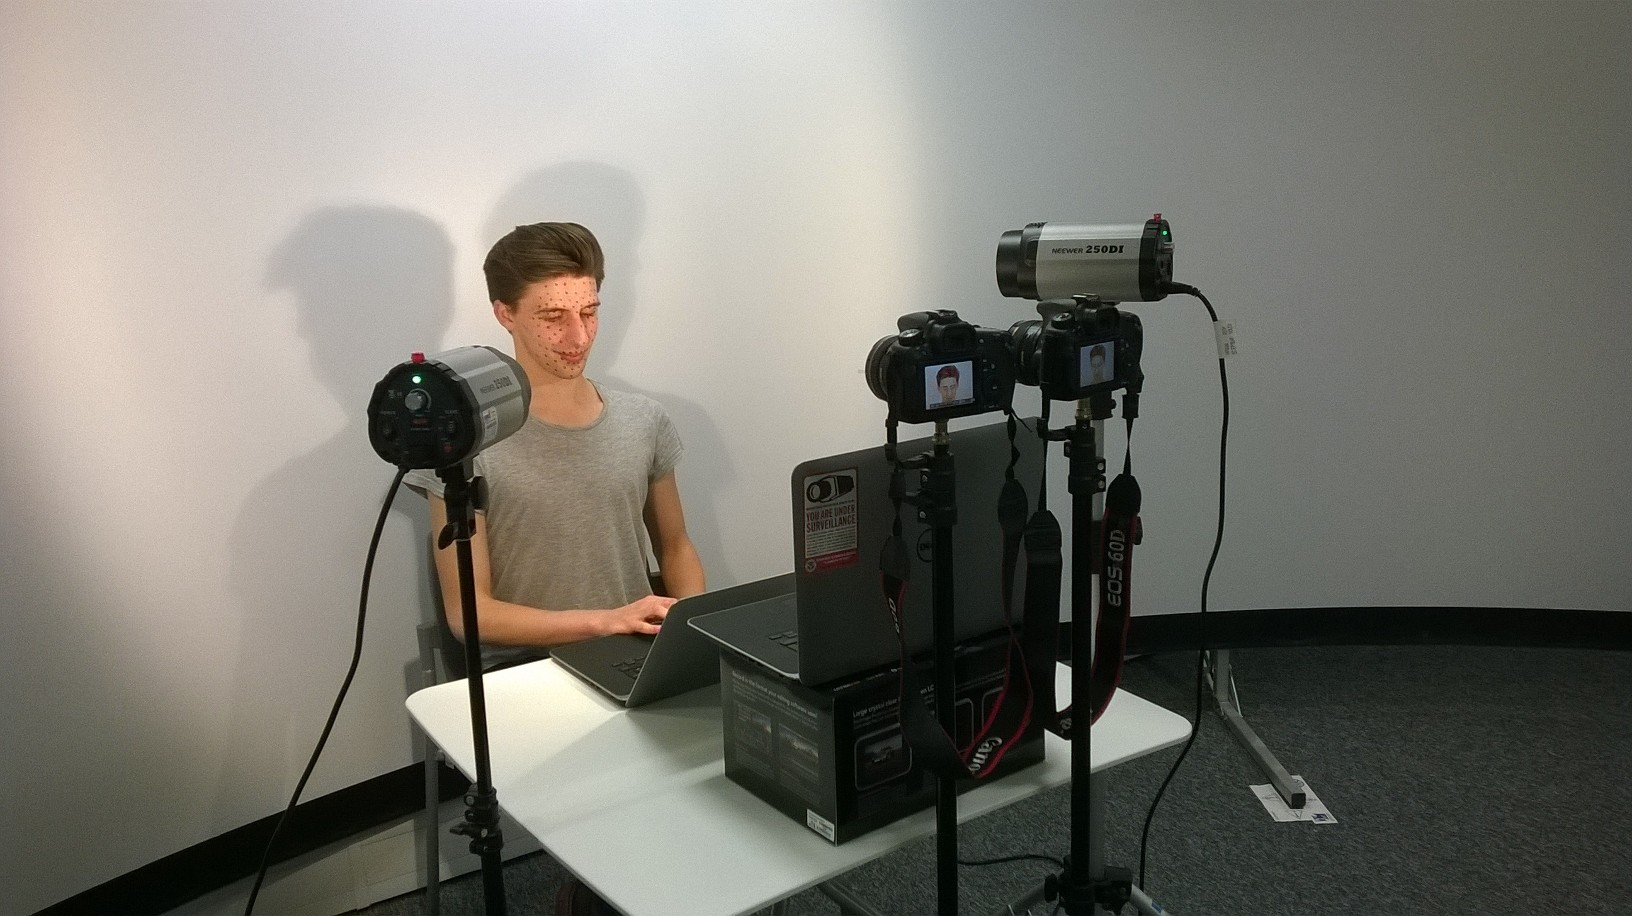
\includegraphics[width=\textwidth]{img/setup1}
	\caption{The stereo camera setup used to capture the facial performance.}
	\label{fig:setup1}
\end{figure}

Markers used to track the facial performance were placed on the face in the configuration shown in Figure \ref{fig:facemarkers}. 97 markers were used in total, and were drawn onto the actor's face with a makeup pencil so as to be easily removed after the capture session. The positions of the markers were roughly based on those used in the Surrey Audio-Visual Expressed Emotion (SAVEE) Database ~\cite{Surrey}, as shown in Figure \ref{fig:surreydata}, although they use fewer markers with 60 in total. In hindsight, using slightly fewer number of markers might have been preferable, as consistently detecting and tracking a large number of markers became quite time-consuming and labour intensive. Furthermore, rather than simply using a black pencil, it might have advantageous to use markers of a significantly different colour to the tones of the human face in order to aid marker detection and tracking, perhaps even using retro-reflective markers as in many commercial motion capture systems ~\cite{Vicon}.

\begin{figure}[htbp!]
\begin{minipage}[b]{0.47\textwidth}
\centering
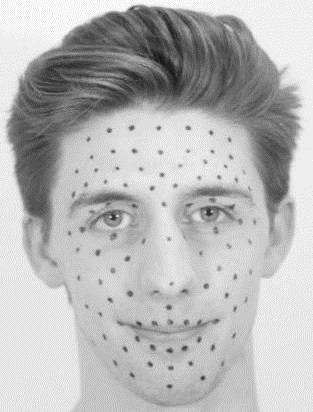
\includegraphics[width=\textwidth]{img/facemarkers}
	\caption{ The configuration of markers used for tracking the facial performance of the actor.}
	\label{fig:facemarkers}
\end{minipage}
\hfill
\begin{minipage}[b]{0.5\textwidth}
\centering
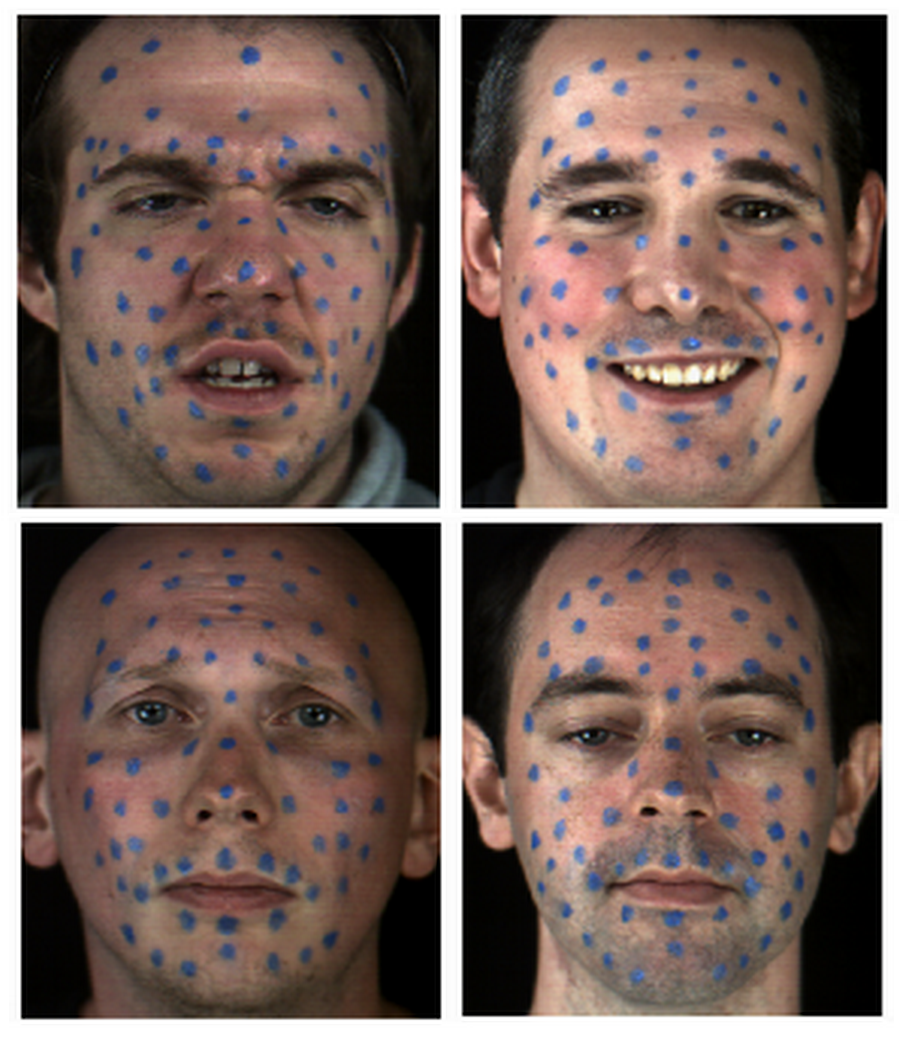
\includegraphics[width=\textwidth]{img/surreydata}
	\caption{ Images from the Surrey Audio-Visual Expressed Emotion (SAVEE) Database ~\cite{Surrey}.}
	\label{fig:surreydata}	
\end{minipage}
\end{figure}


\section{Camera Calibration}

In order to obtain the 3D coordinates of the markers on the face, the cameras first needed to be calibrated. This was achieved using a checkerboard pattern held in a number of different positions in front of both cameras simultaneously, as shown in Figure \ref{fig:checkerboard}. We made use of the Camera Calibration Toolbox for Matlab \cite{Calib} provided by Jean-Yves Bouguet. It was important to ensure that the checkboard remained within the frame of both cameras during the entire calibration process. 

\begin{figure}[htbp!]
\centering
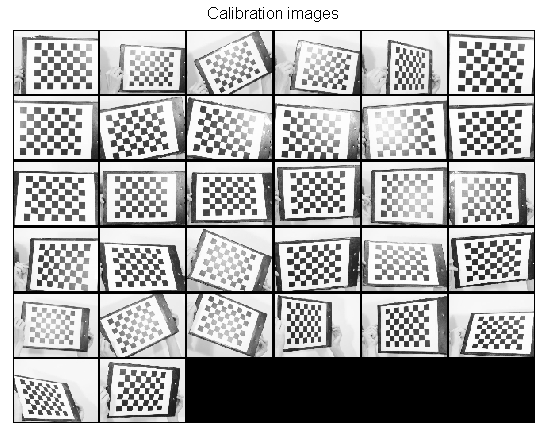
\includegraphics[width=0.6\textwidth]{img/checkerboard}
	\caption{A checkerboard pattern was used to calibrate the pair of stereo cameras.}
	\label{fig:checkerboard}
\end{figure}

As a result of the stereo calibration, we obtain an estimate of the intrinsic and external parameters of the two cameras, from which we can compute the camera projection matrices using the perspective projection equation:

\begin{equation*}
\label{qrdecomp}
	\left(\!
    \begin{array}{c}
      su \\
      sv \\
      s
    \end{array}
  	\!\right) =
  \vect{K}[\vect{R}|\vect{t}]
    \left(\!
    \begin{array}{c}
      X \\
      Y \\
      Z \\
      1
    \end{array}
    \!\right) 		 
\end{equation*}

\begin{equation*}
\left(\!
    \begin{array}{c}
      su \\
      sv \\
      s
    \end{array}
  	\!\right) =
  \begin{bmatrix}
       fk_u & 0 & u_0 \\[0.3em]
       0 & fk_v & v_0 \\[0.3em]
       0 & 0 & 1
  \end{bmatrix}
    \begin{bmatrix}
       r_{11} & r_{12} & r_{13} & t_x \\[0.3em]
       r_{21} & r_{22} & r_{23} & t_y \\[0.3em]
       r_{31} & r_{32} & r_{33} & t_z
  \end{bmatrix}
    \left(\!
    \begin{array}{c}
      X \\
      Y \\
      Z \\
      1
    \end{array}
    \!\right)
\end{equation*}


The resulting extrinsic parameters, describing the rotation and translation between the views, are visualised in Figure \ref{fig:calib}.

\begin{figure}[htbp!]
\centering
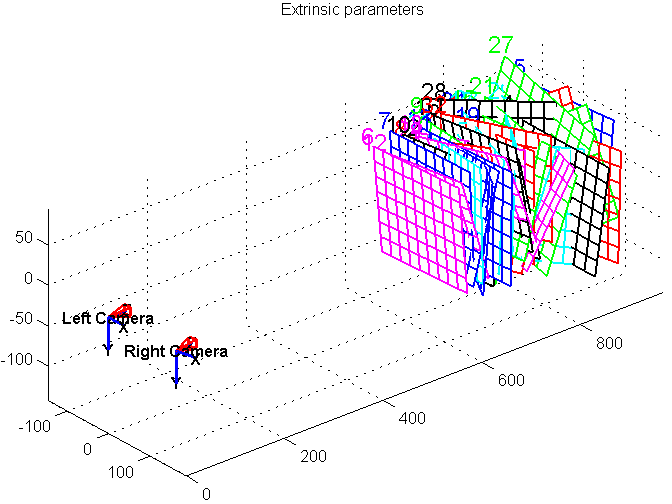
\includegraphics[width=0.8\textwidth]{img/calib}
	\caption{The resulting extrinsic parameters of the calibrated stereo camera setup.}
	\label{fig:calib}
\end{figure}

Given the estimated camera projection matrices, we can then rectify the stereo images for every frame from a captured image sequence, so that the eipolar lines are horizontal. This reduces the stereo matching problem to a 1D search problem, as the same 3D is constrained to lie on the same pixel row in each pair of images. A pair of rectified images and corresponding epipolar lines are shown in Figure \ref{fig:epipolarlines}.

\begin{figure}[htbp!]
\centering
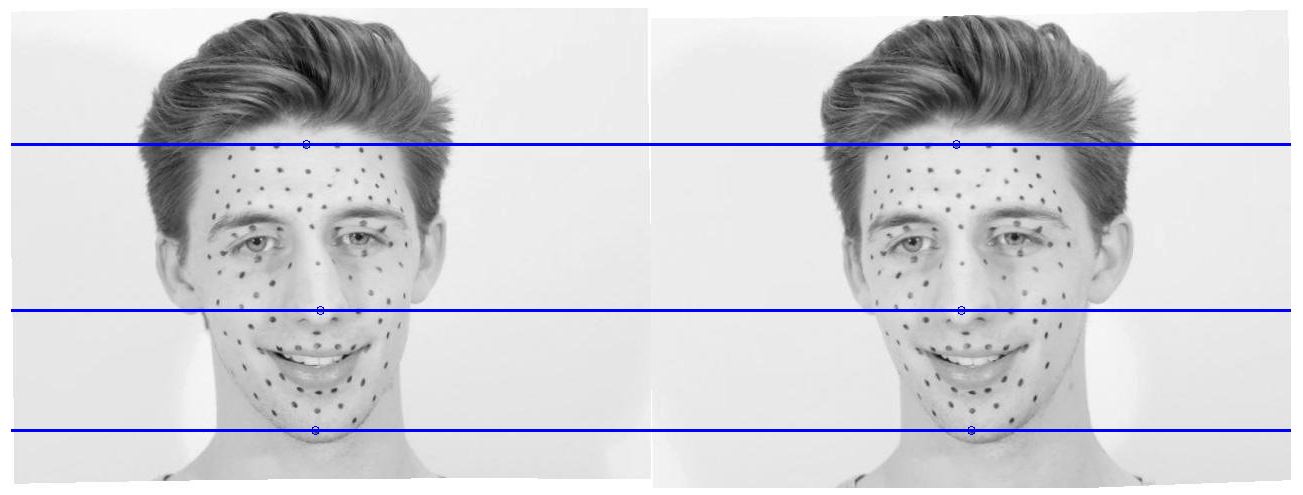
\includegraphics[width=\textwidth]{img/epipolarlines}
	\caption{Using the stereo calibration results, each pair of images in a captured image sequence is rectified so that corresponding epipolar lines lie on the same pixel row. This reduces the stereo correspondence problem to a 1D search along the epipolar lines.}
	\label{fig:epipolarlines}
\end{figure}

\section{Initial Marker Detection}

The facial markers are detected in the first frame of a captured image sequence and then are tracked throughout the length of the sequence. The initial marker detection is achieved by detecting SIFT features in the image. We employ the open source Matlab implementation VLFeat \cite{vedaldi08vlfeat} to do this. 

The marker detection process for the first frame of a given stereo image sequence is carried out as follows. First the user defines a region of interest in the left image around the face of the actor to be tracked, by drawing a contour in the image. We make use of the Matlab function \texttt{roipoly} for this. Then, SIFT features are detected within the selected image region, choosing the appropriate SIFT parameters to pick out features of around 5 pixels in diameter - this may take a few tries to get right. Once reasonable SIFT features have been detected, additional feature points can then be added manually, and also wrongly detected points can be removed, by interactively selecting certain points the user wishes to change. Once the user has successfully detected all 97 facial markers in the left image, the corresponding marker positions are found in the right image by searching along the corresponding epipolar lines; simply the same row of pixels in the right image since the images have been stereo rectified beforehand. The matching points in the right image are found by computing the normalised cross-correlation between image patches:

\begin{equation}
\begin{aligned}
	C_{NCC} = \sum_{i=1}^N \frac{(I_i^L - \mu^L)(I_i^R - \mu^R)}{\sigma^L \sigma^R}
\end{aligned}
\end{equation}

\begin{figure}[htbp!]
\centering
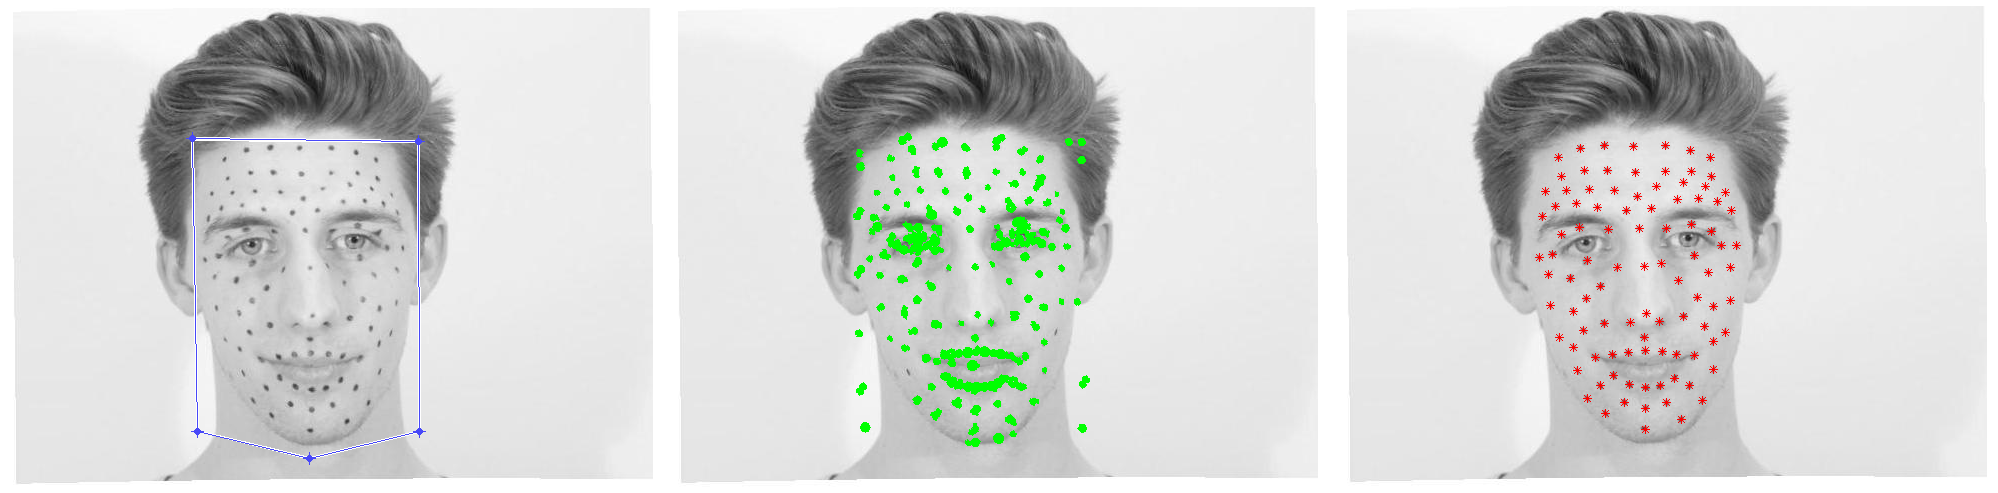
\includegraphics[width=\textwidth]{img/detection}
	\caption{Facial markers are detected by first selecting a region of interest, detecting SIFT features, and then removing unwanted points or adding additional points.}
	\label{fig:detection}
\end{figure}

\begin{figure}[htbp!]
\centering
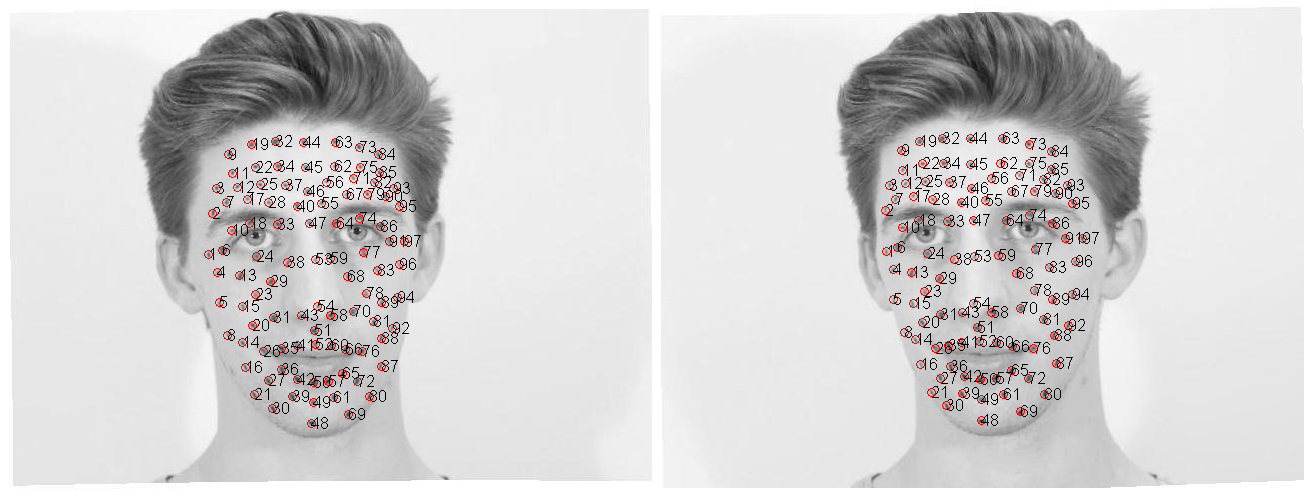
\includegraphics[width=\textwidth]{img/matching}
	\caption{Detected facial markers in the left image are matched to markers in the right image pair by computing the normalised cross-correlation between image patches around the points.}
	\label{fig:matching}
\end{figure}

\section{Marker Tracking}

With the facial markers detected in the first frame, the next task was to track the positions of the markers as they move throughout the image sequence. 

\subsection{Optical Flow}

\subsection{KLT Tracker}

\cite{Shi:1994}

\subsection{Kalman Filter}

\section{Sparse Facial Reconstruction}

Once we have obtained the 2D image coordinates of the facial markers for every frame in a stereo image sequence, we then compute the sparse 3D reconstruction over the sequence. In one frame, given a pair of image correspondences $\vect{w} = (u,v,1)^T$ and $\vect{w}' = (u',v',1)^T$ of the same 3D point $\vect{X} = (X,Y,Z,1)^T$, we can write two equations using the projection matrices $\vect{P}$ and $\vect{P'}$:

\begin{equation}
\left(\!
    \begin{array}{c}
      su \\
      sv \\
      s
    \end{array}
  	\!\right) = \vect{P}
  	\left(\!
    \begin{array}{c}
      X \\
      Y \\
      Z \\
      1
    \end{array}
  	\!\right) 
  	\ \ \ \ \ \ \ \ 
\left(\!
    \begin{array}{c}
      su' \\
      sv' \\
      s
    \end{array}
  	\!\right) = \vect{P'}
  	\left(\!
    \begin{array}{c}
      X \\
      Y \\
      Z \\
      1
    \end{array}
  	\!\right).
\end{equation}
For each pair of image points, two equations can be written:

\begin{align*}
u &= \frac{p_{11}X + p_{12}Y + p_{13}Z + p_{14}}{p_{31}X + p_{32}Y + p_{33}Z + p_{34}} \ \  
u' = \frac{p'_{11}X + p'_{12}Y + p'_{13}Z + p'_{14}}{p'_{31}X + p'_{32}Y + p'_{33}Z + p'_{34}}\\ 
v &= \frac{p_{21}X + p_{22}Y + p_{23}Z + p_{24}}{p_{31}X + p_{32}Y + p_{33}Z + p_{34}} \ \ 
v' = \frac{p'_{21}X + p'_{22}Y + p'_{23}Z + p'_{24}}{p'_{31}X + p'_{32}Y + p'_{33}Z + p'_{34}}
\end{align*}
Rearranging, these can be written in the form $\vect{AX} = 0$ as follows, where $\vect{p}_i$ denotes the $ith$ row of the projection matrix $\vect{P}$

\begin{equation}
\begin{bmatrix}
       u\vect{p}_3^T - \vect{p}_1 \\[0.3em]
       v\vect{p}_3^T - \vect{p}_2 \\[0.3em]
       u' \vect{p'}_3^T - \vect{p'}_1 \\[0.3em]
       v' \vect{p'}_3^T - \vect{p'}_2
\end{bmatrix}
\left(\!
    \begin{array}{c}
      X \\
      Y \\
      Z \\
      1
    \end{array}
  	\!\right) = 0.
\end{equation}
Two equations are acquired from each image point in the two views, giving a total of four equations with three unknowns - the problem is over-constrained. A linear least-squares solution can be found by performing Singular Value Decomposition on the matrix $\vect{A}$. The 3D coordinates of the point $\vect{X}$ are the singular vector corresponding to the smallest singular value of $\vect{A}$, i.e. the last column of the matrix $\vect{V}$, where $\vect{A} = \vect{UDV}^T$. This is implemented in Matlab in the function \texttt{Reconstruct.m}, which takes in the two camera projection matrices for a pair of stereo cameras and the matching 2D image points, and returns an array of corresponding 3D points.

\begin{figure}[htbp!]
\centering
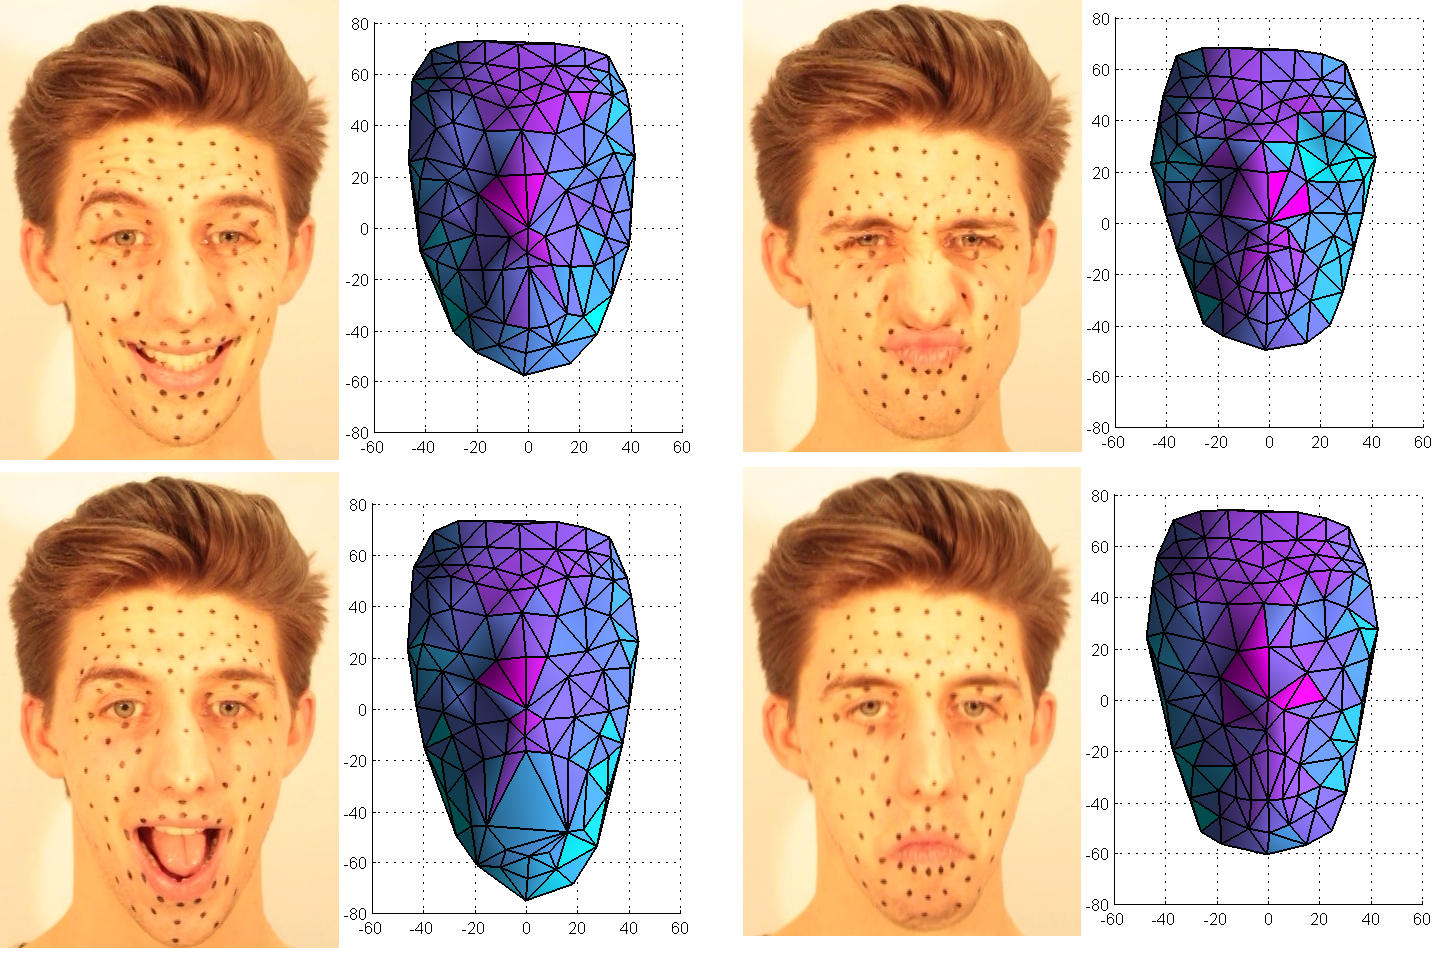
\includegraphics[width=\textwidth]{img/faces}
	\caption{A sparse 3D reconstruction is computed for every frame of an image sequence using the detected marker positions and the calibrated camera projection matrices. A sample of image frames and the corresponding 3D reconstructions are shown above.}
	\label{fig:faces}
\end{figure}

\subsection{Stabilising Head Movement}
\label{sec:stabilising_head_movement}

It is important for the actor's head to remain still throughout the sequence so that the reconstructed facial expressions are expressed as true non-rigid deviations from the neutral facial expression. Proper stabilisation of the head is required to avoid artefacts in the resulting blendshape facial animation and retargeting process \cite{Beeler:2014}. If the rigid head movement is not removed, then the expression shapes will contain this 'baked-in' rigid motion, and any facial animation constructed from the expressions will also contain this unwanted rigid head motion. In industry, face-stabilisation is still usually performed manually; Weise \textit{et al}. \cite{Weise:2009} aim to remove the rigid motion component of multiple expressions using ICP registration and Vlasic \textit{et al}. \cite{Vlasic:2005} use Procrustes alignment.

In our implementation, we attempt to remove the majority of the actor's rigid head motion by performing a Procrustes analysis \cite{Gower:1975} using a number of approximately rigid points. At least four points are required for the Procrustes alignment. The rigid points were chosen to be the tops of the ears, the tip and bridge of the nose, and the centre point on the top of the forehead, as shown by the dots in Figure \ref{fig:procrustes}. However, none of these points are actually truly rigid, so this is just an approximation to the true stabilisation. In a future implementation, it would be better to actually track a few points known to be practically rigid, for example by placing markers on the top of the head. 

The Procrustes analysis computes a least-squares fit of each facial expression in a given frame to the neutral face, given the rigid vertex correspondences. In Figure \ref{fig:procrustes}, the rigid correspondences are plotted in red for the neutral face, and blue for a particular frame. We do this for the entire image sequence so that in every frame the head pose is aligned to the neutral position. We have found that the average error over an image sequence is usually around the order of $10^{-3}$. However, it is not simply the case that the smaller the error means the better the alignment of the expression to the neutral face, because the head can be orientated in such a way that can make the error in the rigid vertex correspondences small, but can result in an unnatural head pose. Through experimentation, we have found that choosing points that span the entire face and are placed the extremities of the face, such as the ears, generally results in a better alignment than rather selecting a few points close together around the centre of the face, such as around the mostly rigid nose region. This makes sense because a small deviation in points around the centre of mass will lead to larger displacements in the other points, whereas small deviations in points at the edges will have much less of an impact on points in the centre of the face. 

\begin{figure}[htbp!]
\centering
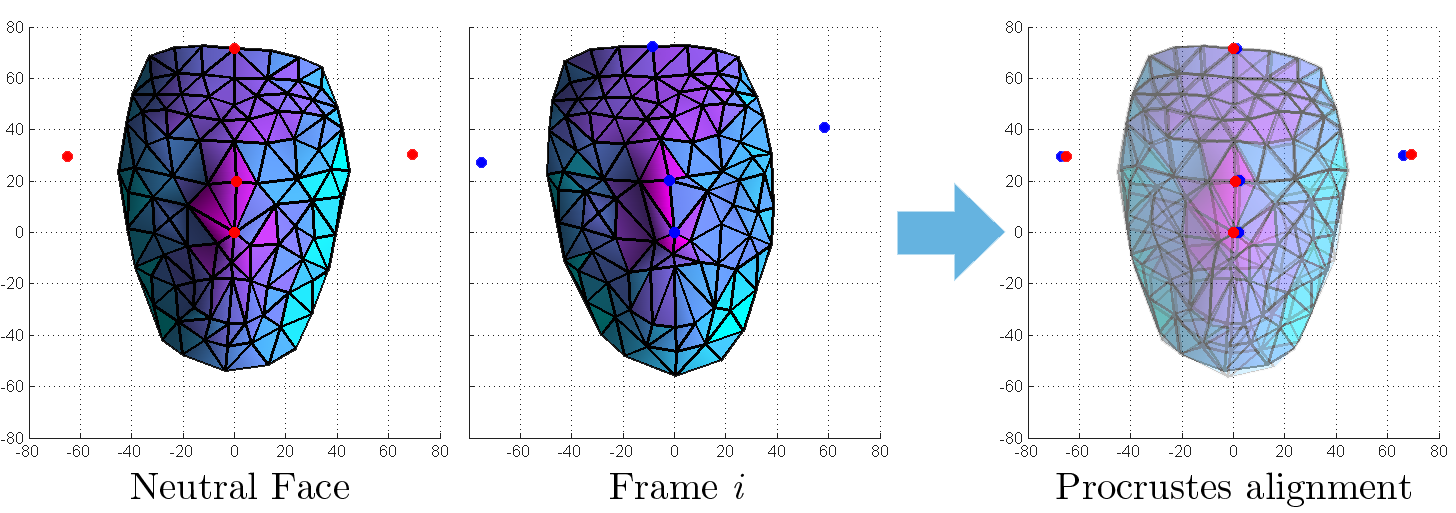
\includegraphics[width=\textwidth]{img/procrustes}
	\caption{The head pose in each frame of an image sequence is aligned to the neutral face position using Procrustes analysis. The rigid vertex correspondences are shown in red for the neutral pose, and blue for a given frame.}
	\label{fig:procrustes}
\end{figure}

\section{Facial Animation}
Given the motion capture data, our goal is to produce an animation that resembles the captured motion. We use the Digital Emily model designed by Alexander et al.~\cite{Alexander:2009}. In this section we introduce the techniques used to match three-dimensional surfaces and point clouds, and the optimisation methods used to estimate the parameters that describe the motion of the digital model.

\subsection{Thin Plate Splines}\label{sec:tps}
Thin plate theory addresses problems that commonly arise in areas of natural sciences and engineering when trying to model the behaviour of a thin sheet of some material. The possible processes include but are not limited to stretching, bending, crumpling, buckling, shrinking, straining and tearing. The corresponding mathematical model is based on ideas from differential geometry as well as continuum mechanics, and the set of equations describing the aforementioned phenomena are often notoriously difficult to solve. Therefore, in Computer Graphics, as well as other fields, a number of simplifying assumptions are made when constructing a thin plate model. 

A thin plate is considered to be a two dimensional object, i.e. it is assumed that the thickness is infinitesimal. The geometry of the object is often simplified to reduce the computational cost. Thin plate splines (TPS) are a two-dimensional counterpart of the cubic spline~\cite{Sibson:1991}. TPS are a deformation method based on the assumption that a thin surface deforms in a way that minimises the surface bending energy. The bending energy is proportional to the change in the second fundamental form. Specifically, given two corresponding sets of point $\{(x_i, y_i\}_i^N$ and $\{v_i\}_i^N$ there exists a height field mapping between the two, $f: \mathbb{R}^2 \to \mathbb{R}$. The bending energy corresponding to this mapping is proportional to the second order derivatives of the mapping:
\begin{equation}
\begin{aligned}
	E_{bend}(f) = \lambda \iint \left( \left( \dfrac{\delta^2f}{\delta x^2} \right)^2 +  2 \left( \dfrac{\delta^2f}{\delta x y} \right)^2 +  \left( \dfrac{\delta^2f}{\delta y^2} \right)^2 \right) \dd x \dd y,
\end{aligned}
\end{equation} where $\lambda$ is smoothing parameter, which balances the quality of fit and the amount of bending, i.e. the wiggliness of the function. TPS finds the transformation that fits the data while minimising the bending energy. Note that TPS may also be defined in terms of the radial basis functions that are used for smooth scattered data fitting. The RBF solution for thin plate splines is:
\begin{equation}
\begin{aligned}
	f(x,y) = \sum_{i=1}^N \omega_i \: \phi(\|(x,y) - (x_i,y_i)\|), \: \text{ where} \: \phi(r) = r^2 \log(r).
\end{aligned}
\end{equation} To ensure that the function $f$ has square-integrable second derivatives, the following conditions are imposed:
\begin{equation}
	\sum_{i=1}^N \omega_i = \sum_{i=1}^N \omega_i x_i = \sum_{i=1}^N \omega_i y_i = 0.\label{eq:TPSrestrictions}
\end{equation} These conditions and the data fitting requirement may be combined into a linear system of equations:
\begin{equation}
\begin{bmatrix}
	K & P \\
	P^T & 0 
\end{bmatrix} 
\begin{bmatrix}
	\omega \\
	o
\end{bmatrix} = 
\begin{bmatrix}
	v \\
	o
\end{bmatrix}, 
\end{equation} where $K$ encodes the relation between the data points, i.e. $K_{ij} = \phi(\|(x_i,y_i) - (x_j,y_j)\|)$, $P_{i\cdot} = (1, x_i, y_i)$ contains the variables from Eq.~\ref{eq:TPSrestrictions}, $\omega$ contains the values of $\omega_i$, and $v$ contains the target function values $v_i$. The variables $0$ and $o$ denote the zero matrix and the zero column vector respectively. Solving this linear system of equations gives the desired transformation in two dimensions. The method extends naturally to three-dimensional problems by including a dependence on an additional variable in the calculations described above. Radial basis functions are commonly used in the field of performance-driven animation~\cite{Joshi:2003}.

\subsection{Non-Rigid ICP}
Iterative Closest Point (ICP) is an algorithm used to align two partially overlapping point clouds by minimising the square error between corresponding points. The quality of the results produced by this algorithm is sensitive to the initial guess at a solution, i.e. ICP only refines the initial estimation. See Alg.~\ref{alg:icp} for the outline of the algorithm. Mean square error algorithm is used to calculate the average of the squared errors between the target and the transformed source points. Thus the objective function is a function of rotations and translations. The output of the algorithm is a transformation matrix that provides the optimal mapping between the two point clouds within a given threshold. The transformation matrix may be split into rotation and translation. The algorithm solves a linear system of equations where the unknowns are the coefficients in the rotation matrix and the translation vector and the known point cloud values are used as coefficients. The method is often used to find a transformation between a point cloud and a surface; in that case the surface normals are used as additional input.

\begin{algorithm}[H]   \caption{Iterative Closest Point.}
\KwData{source point cloud \\
\hspace{0.9cm} target point cloud\;
\hspace{0.9cm} initial guess\;
\hspace{0.9cm} error threshold\;
 }
\BlankLine
\While{error $>$ threshold}{
\For{point in source}{
  find closest point in target\;
  }
use mean squared error to find best transformation that aligns source to target \;
apply transformations\;
}
 \label{alg:icp}
\end{algorithm} 
The original ICP algorithm is limited to rigid transformations, i.e. rotation and translation, which have only $6$ degrees of freedom. However, in order to capture scaling, shearing and other more complicated transformation, an affine mapping should be used. Thus an extension of the ICP algorithm, called non-rigid ICP is used when additional degrees of freedom are present. Allen et al. proposed a non-rigid registration method that uses a numerically non-linear solver to find a smooth affine mapping~\cite{Allen:2003}. Additional constrained are imposed by manually matching some known marker locations in the two datasets. The method exhibits slow convergence and often leads to local minima; consequently, the authors use a multi-resolution approach where the optimisation is first performed on a low resolution mesh, and then optimised on the high resolution mesh. Amberg et al. combined the ICP algorithm with the method of Allen et al. to overcome the issues with convergence~\cite{Amberg:2007}.

\subsection{Animation}
The aim of this project is to used captured data of a face to animate a given model. We use the digital Emily model that comes with $68$ controllable blendshapes ranging from simple eyebrow movements to complicated lip corner pulls~\cite{Alexander:2009},~\cite{FaceWareRigsWeb}. Each blendshape has a weight $w_i$ associated with it, and $w_i \in [0,1]$. The model includes eyes and teeth. The aim is to find a combination of these blendshapes that produce a specified facial expression. In particular, we are interested in reproducing the captured sequence of expressions. 

\subsubsection{Initial Approach}
We manually choose a sparse set of points that corresponds to the sparse source mesh. Then the neutral expression of the subject is matched with the neutral expression of Emily by transforming the sparse source mesh to the sparse target mesh using TPS. The transformation is stored, and it is used to map all the frames in the captured sequence. This produces a sparse Emily sequence; using TPS again we warp the dense Emily mesh according to the positions of the sparse points. The quality of the resulting animation is poor for a number of reasons. Firstly, the sparse points are not able to constrain the dense mesh, especially since parts of the face, for example the eyelids and the lips are not tracked in the sparse mesh. Consequently, numerous artefacts appear on the dense mesh, and they are particularly noticeable around the lips as no boundary conditions are imposed. Secondly, though there is a clear correspondence between the generated Emily sequence and the source sequence, the generated expressions look unnatural. This may be explained by the differences in the geometry and anatomy of the two faces; for instance, the source may be able to pull expressions that cannot be mimicked by the model. In addition, the errors in tracking, reconstruction, and manual selection of sparse points on Emily further reduce the quality of the animation.

Our initial attempt to improve the method involved simplifying the dense Emily model by removing the part of the mesh that corresponds to the lips. Though the simpler mesh exhibited slightly better behaviour, i.e. there were fewer visible artefacts, the sparse point cloud was still unable to constrain the dense mesh well enough to produce realistic results, see Fig.~\ref{fig:ghost}. 
\begin{figure}[htbp!]
        \centering
        \begin{subfigure}[b]{0.45\textwidth}
                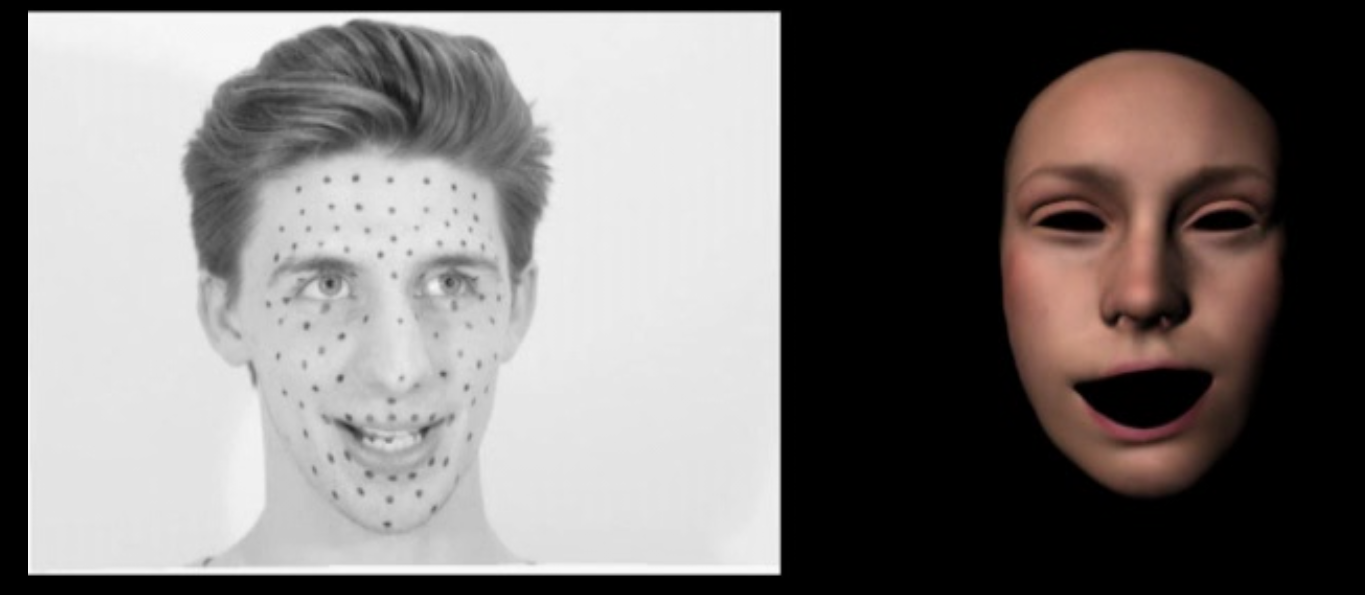
\includegraphics[width=\textwidth]{img/ghost1.png}
        \end{subfigure}
        \begin{subfigure}[b]{0.45\textwidth}
                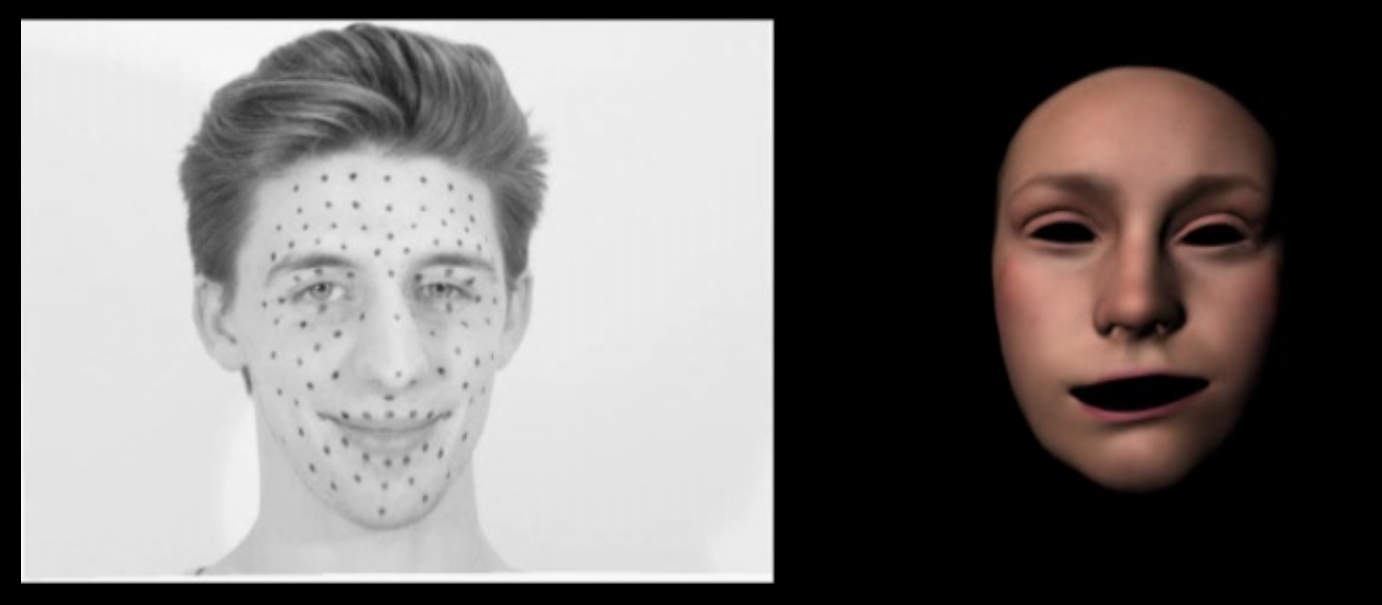
\includegraphics[width=\textwidth]{img/ghost2.png}
        \end{subfigure}
        \caption{Our first animation produced by warping the ector's expressions at each frame of the sequence. }\label{fig:ghost}
\end{figure}

\subsubsection{Introduction of Blendshapes}
In an attempt to improve the visual quality of the generated animation, we decided to use a set of Emily key-shapes, that were readily available to us. The main argument for using these blendshapes is that in most situations a simple linear relation exists between an arbitrary facial expression and the set of key-shapes. The shape may encode the entire geometry of the case, the displacement from the neutral face, or the local features of a face. If no such shapes are available, they may be producing using PCA. Such set of blendshapes is orthogonal, thus the features encoded by each shape are controlled independently; however, such shapes do not allow for intuitive facial transformations making it difficult to perform manual post-process editing.

Let us define a set of blendshapes $\mathbf{B} = [\bb_0, \ldots, \bb_n]$ where $\bb_0$ is the mesh of a neutral face, and each of the $\bb_i$ correspond to a basic facial expression, for example the raise of an eyebrow. Unless stated otherwise, we shall use $68$ shapes provided with the digital Emily model. Then a new facial expression $\mathbf{F(\w)}$ may be constructed by finding an appropriate linear combination of the offsets of the basic shapes:
\begin{equation}
	\F(\w) = \bb_0 + \sum_{i=1}^N w_i \: |\bb_i - \bb_0|, \label{eq:blendshapes}
\end{equation} where $\w = [w_1, \ldots, w_n]$ is a set of weights that describe how much each of the basic shapes affect the new expression $\mathbf{F(\w)}$. Typically, a convexity constraint is imposed on the weights; in our case the choice of constraints is influenced by the constraints present in our blendshape model, i.e. $w_i \in [0,1]$. Eq.~\ref{eq:blendshapes} may be written as a linear system of equations as follows:
\begin{equation}
	\F(\w) - \bb_0 = \hat{\mathbf{B}} \w, \label{eq:linsyst}
\end{equation} where $\hat{\mathbf{B}}$ is the original set of blendshapes without the neutral expression. 

A number of different numerical optimisation methods where tested when solving for the blendshape weights. An unconstrained solution may be calculated by inverting matrix $\hat{\mathbf{B}}$, and multiplying it from the left with the left hand side of Eq.~\ref{eq:linsyst}. Instead we use Matlab's constrained non-negative least-squares solver (\texttt{lsqnonneg}) and constrained linear least-squares solver (\texttt{lsqlin})~\cite{Matlab}. For the non-negative least-squares solver we formulate our problem as follows:
\begin{equation}
	\min_\w \| \hat{\mathbf{B}} \w - (\F(\w) - \bb_0) \|_2^2, \: \w_i \geq 0, \: i = 1, \ldots, n. \label{eq:lsqnonneg}
\end{equation} The solver uses an active set method, and iteratively improves the active set of basis vectors; it converges in finite time. The same formulation is used for the linear least squares solver though it includes an additional upper limit on the argument. This solver uses a reflexive Newton method which is able to accurately locate the local minimisers of large systems, and exhibits global convergence. It is also able to maintain sparsity of matrices but is generally slower.

\subsubsection{Two-dimensional Sequence}

Our initial tests of the optimisation algorithms were carried out on a two-dimensional sequence of facial motion. Approximately $90$ points on a sequence were marked and tracked to produce a sparse motion sequence. Then a set of key frames were hand-picked to represent the extreme cases of the facial motion, see Fig.~\ref{fig:2Dblends}. The sparse points from these frames are then used as blendshapes. The two solvers were tested on the entire motion sequence. We shall compare the results by estimating the average error between the pixels in the original sequence and the weighted sequence.

Fig.~\ref{fig:frame10} and Fig.~\ref{fig:frame400} illustrate the concept of blendshapes. Frame $10$ is very close to one of the blendshapes, and both optimisation methods are able to represent this expression well; the average error associated with the constrained non-negative least-squares solver is less than $0.29$, which corresponds to approximately $0.01$ centimetres, while the average error for the second solver is less than $0.21$ or approximately $0.09$ centimetres. Note that as expected both methods use frame $9$ with a large weight. However, the other blendshapes are different for the two methods. This suggests that none of the blendshapes is able to capture the subtle change between frames $9$ and $10$. In comparison, frame $400$ is twelve frames away from a frame that was chosen as a blendshape, resulting in an increase in average error for the two methods (approximately 0.49 in both cases). As expected, both methods use the two blendshapes that are the nearest to frame $400$ in terms of timing. The weights used for these two shapes are the same to three significant digits, and the extra shape used by the first method has a low weight assigned to it. Note that the first method does not obey the restriction of $\sum_{i=1}^N w_i = 1$. Though the second method is able to produce slightly more accurate results, at least for this data set the difference does not seem significant. 

\begin{figure}[htbp!]
\centering
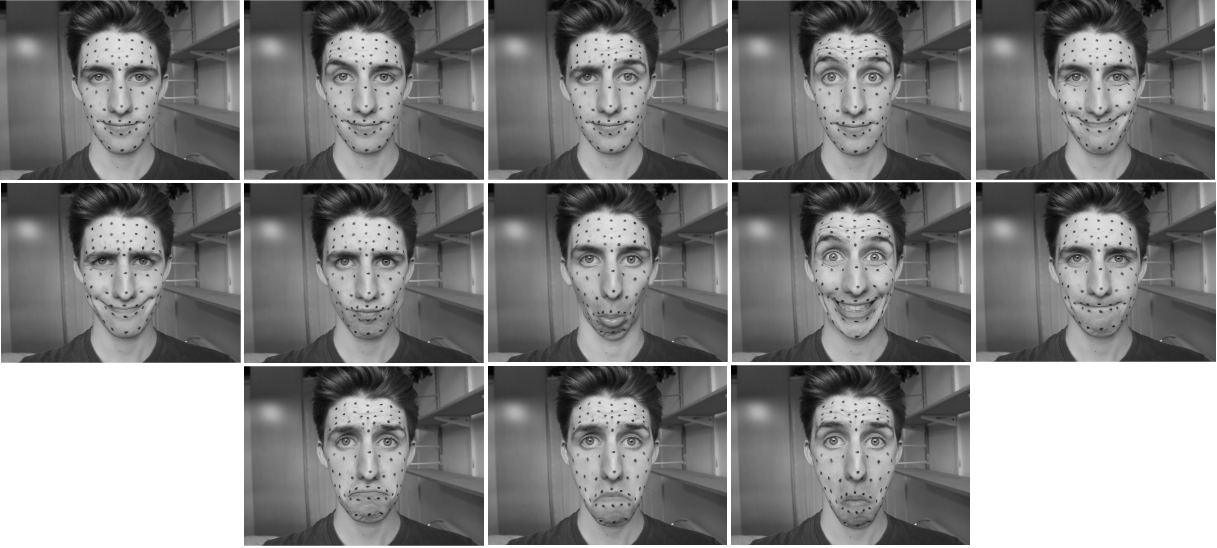
\includegraphics[width=0.8\textwidth]{img/weights/2D/basis/all.png}
	\caption{Set of facial expressions used as blendshapes. The first frame is used as a neutral expression.}
	\label{fig:2Dblends}
\end{figure}
\begin{figure}[htbp!]
\centering
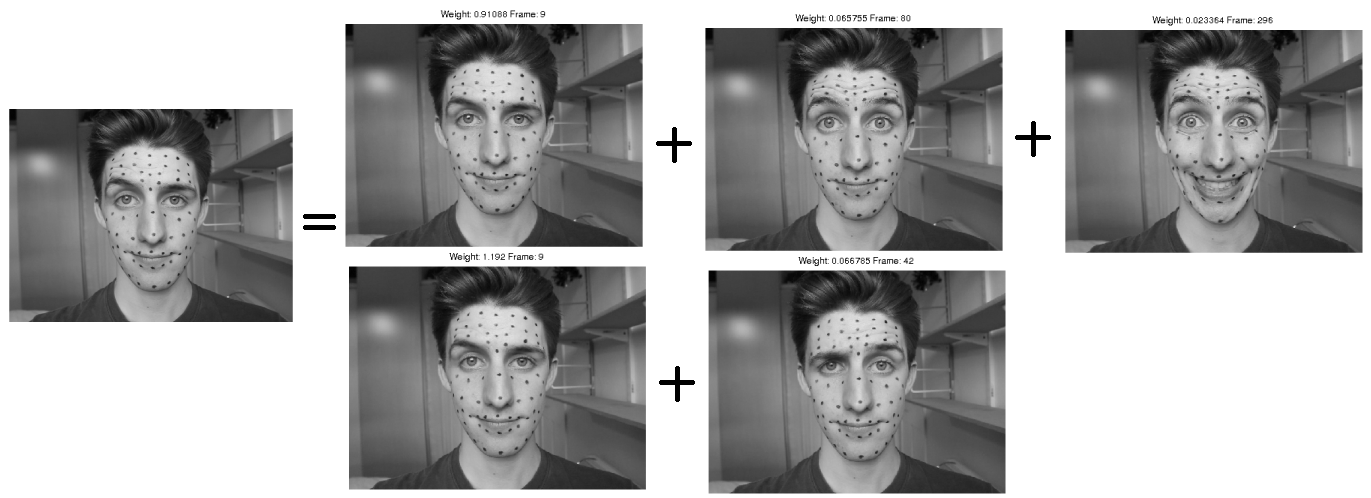
\includegraphics[width=0.8\textwidth]{img/weights/2D/frame_10/all.png}
	\caption{Frame $9$ on the left represented as a linear combination of the key frames. The top solution was obtained using the \texttt{lsqnonneg} solver while the bottom one was obtained using \texttt{lsqlin}.}
	\label{fig:frame10}
\end{figure}

\begin{figure}[htbp!]
\centering
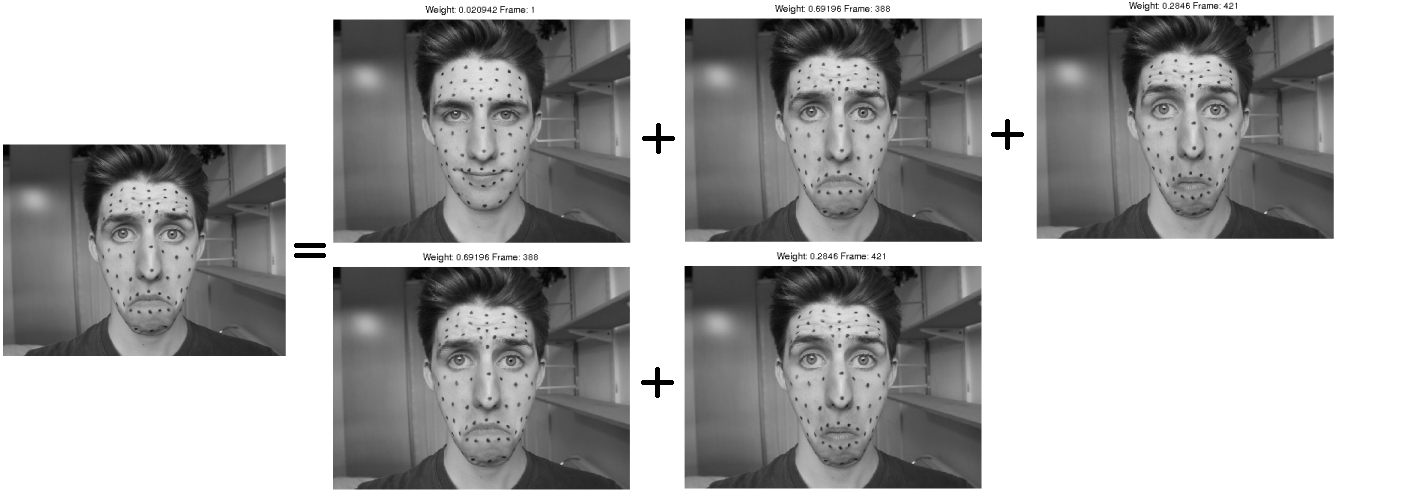
\includegraphics[width=0.8\textwidth]{img/weights/2D/frame_400/all.png}
	\caption{Frame $400$ on the left represented as a linear combination of the key frames. The top solution was obtained using the \texttt{lsqnonneg} solver while the bottom one was obtained using \texttt{lsqlin}.}
	\label{fig:frame400}
\end{figure}
\subsubsection{Principal Component Analysis}

An alternative set of key shapes may be constructed by applying Principal Component Analysis (PCA) to the observed high-dimensional data. Generally, PCA is used to transform a set of correlated observations into a set of values of linearly uncorrelated principal components. If the number of principal components is smaller than the number of original variables, then the method may be used for dimensionality reduction. PCA tries to find a set of orthonormal axes which under projection preserve the highest variance. When formulated as an eigenvalue problem, it finds the eigenvectors of the covariance matrix with the largest eigenvalues. 

PCA has been used in facial animation as an automatic way of constructing a set of blendshapes, see Sec.~\ref{sec:prfacialanimation}. The main advantages of using such blendshapes is that the construction does not require artistic skills, and the shapes are guaranteed to be orthogonal to each other. The second argument is particularly important in compression algorithms, i.e. when the aim is to find the smallest possible set of blendshapes that is able to represent the data while minimising the squared reconstruction error. We use the Matlab implementation of PCA to find a set of PCA eigenvectors that represent the directions with highest variance in our data. Given this new set of shapes, we use the same optimisation algorithm as previously described, replacing the neutral expression with the mean of the data.

To compare the results with a different number of blendshapes, we calculate the average reconstruction error for a $500$ frame sequence. When the first $3$ shapes are used, the error is approximately $0.16$ centimetres and $0.25$ centimetres for the two optimisation methods respectively. Introduction of five additional shapes reduces the error by approximately $0.02$ centimetres. Thus PCA does not outperform the model with manually designed set of key shapes. An additional drawback of the PCA basis is that it is not intuitive, i.e. the key shapes do not correspond to recognisable facial expressions. As a consequence, manual editing of the resulting animation is very complicated. Throughout the rest of the project we use the standard set of $68$ blendshapes from the Digital Emily project.

\subsubsection{Animation of a 3D Model}

Next, we shall consider the animation of the previously introduced three dimensional motion sequence. The captured sequence contains $371$ frames and shows the actor talking from approximately $12$ seconds. The corresponding sequence in the Emily domain is obtained using a linear elasticity method, see Sec.~\ref{sec:tps}. We use a talking sequence that contains $371$ frames. As in the two-dimensional case, at each frame of the sequence, the chosen optimisation method calculates the best possible combination of blendshape weights given the Emily motion sequence. In particular, the input sequence is a sparse sequence of the motion that was transformed from the capture space to the digital model space. 

We start by manually marking the three-dimensional face of Emily; we try to replicate the pattern we used when capturing the actor's face, see Fig.~\ref{fig:facemarkers}. The markers are placed at the vertices of the mesh, and the indices of these vertices are used to find the location of the corresponding markers on the meshes of the blendshapes, see Fig.~\ref{fig:Emarked}. Then the optimisation methods are used to extract the best linear combination of shapes together with the corresponding weights. The average reconstruction error for the non-negative least-squares solver is approximately $0.26$ centimetres, compared to $0.23$ centimetres for the constrained linear least-squares solver, see Fig.~\ref{fig:errorw2w3}. A number of factors may increase the error. Firstly, the expressions captured in Emily blendshapes are fairly mild, i.e. the shapes do not capture the most extreme motion of the face. Consequently, the estimated facial movements may not be expressed as a linear combination of the blendshapes. Secondly, as the blendshapes are not orthogonal, they may combine in unexpected ways, for example cancel each other. This behaviour may be avoided if a set of PCA-produced shapes is used. Also, note that the mesh of Emily is not symmetrical, i.e. the left side of the face does not match the right side. This may lead to a sideways motion that cannot be captured by the blendshapes.
\begin{figure}[htbp!]
        \centering
        \begin{subfigure}[b]{0.25\textwidth}
                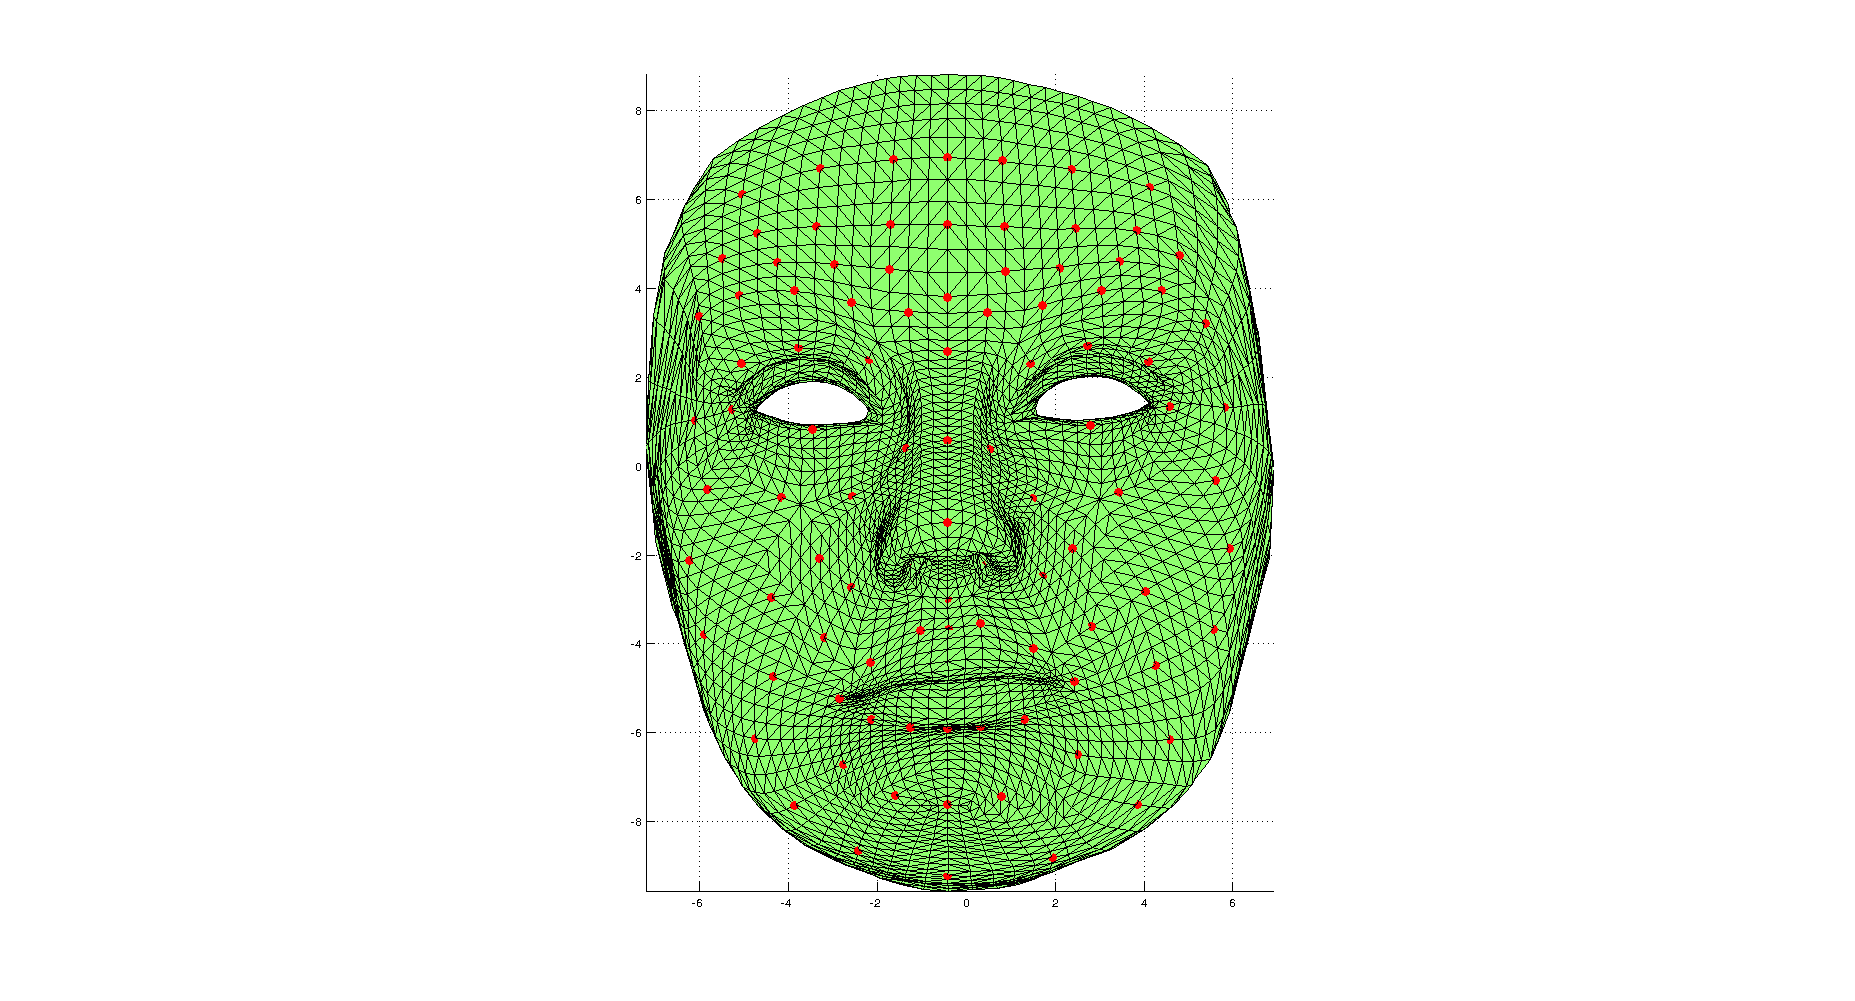
\includegraphics[trim = 160mm 20mm 160mm 10mm, clip,width=0.7\textwidth]{img/weights/3D/Emily_marked/neutralE_marked.png}
        \end{subfigure}%
        ~ %add desired spacing between images, e. g. ~, \quad, \qquad, \hfill etc.
          %(or a blank line to force the subfigure onto a new line)
        \begin{subfigure}[b]{0.25\textwidth}
                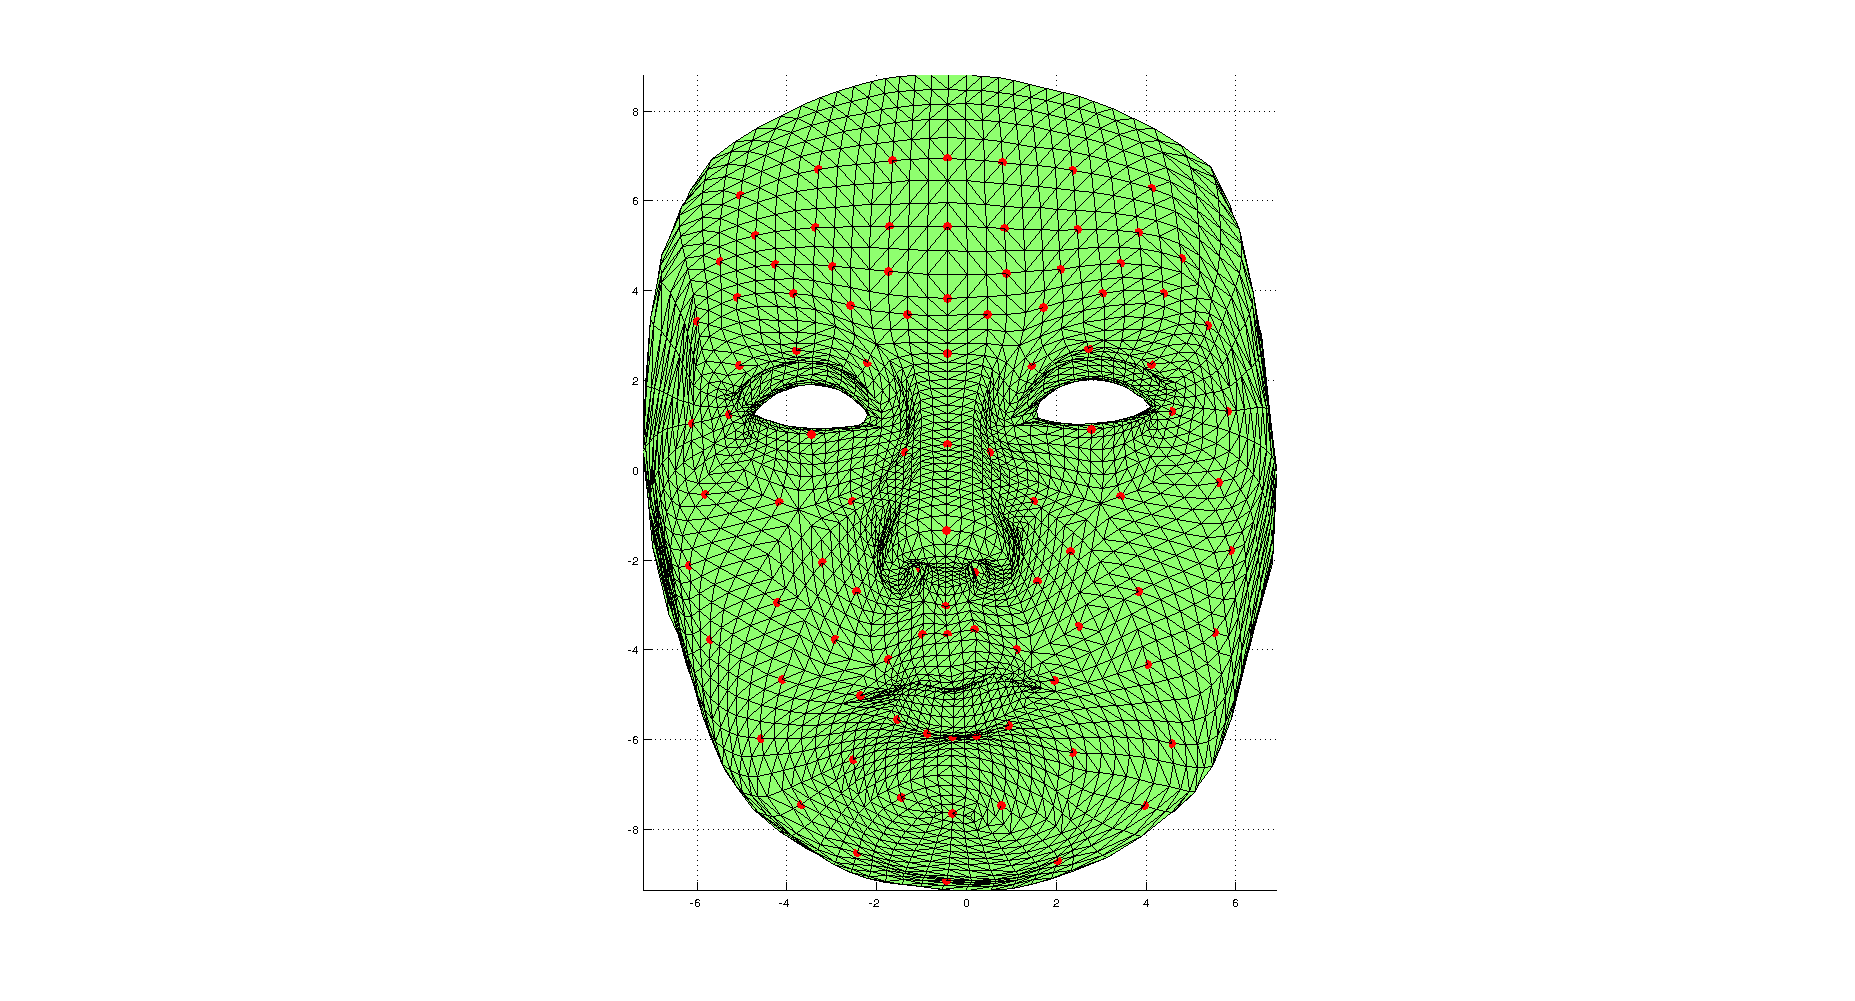
\includegraphics[trim = 160mm 20mm 160mm 10mm, clip,width=0.7\textwidth]{img/weights/3D/Emily_marked/blendshapeE_marked_50.png}
        \end{subfigure}
        ~ %add desired spacing between images, e. g. ~, \quad, \qquad, \hfill etc.
          %(or a blank line to force the subfigure onto a new line)
        \begin{subfigure}[b]{0.25\textwidth}
                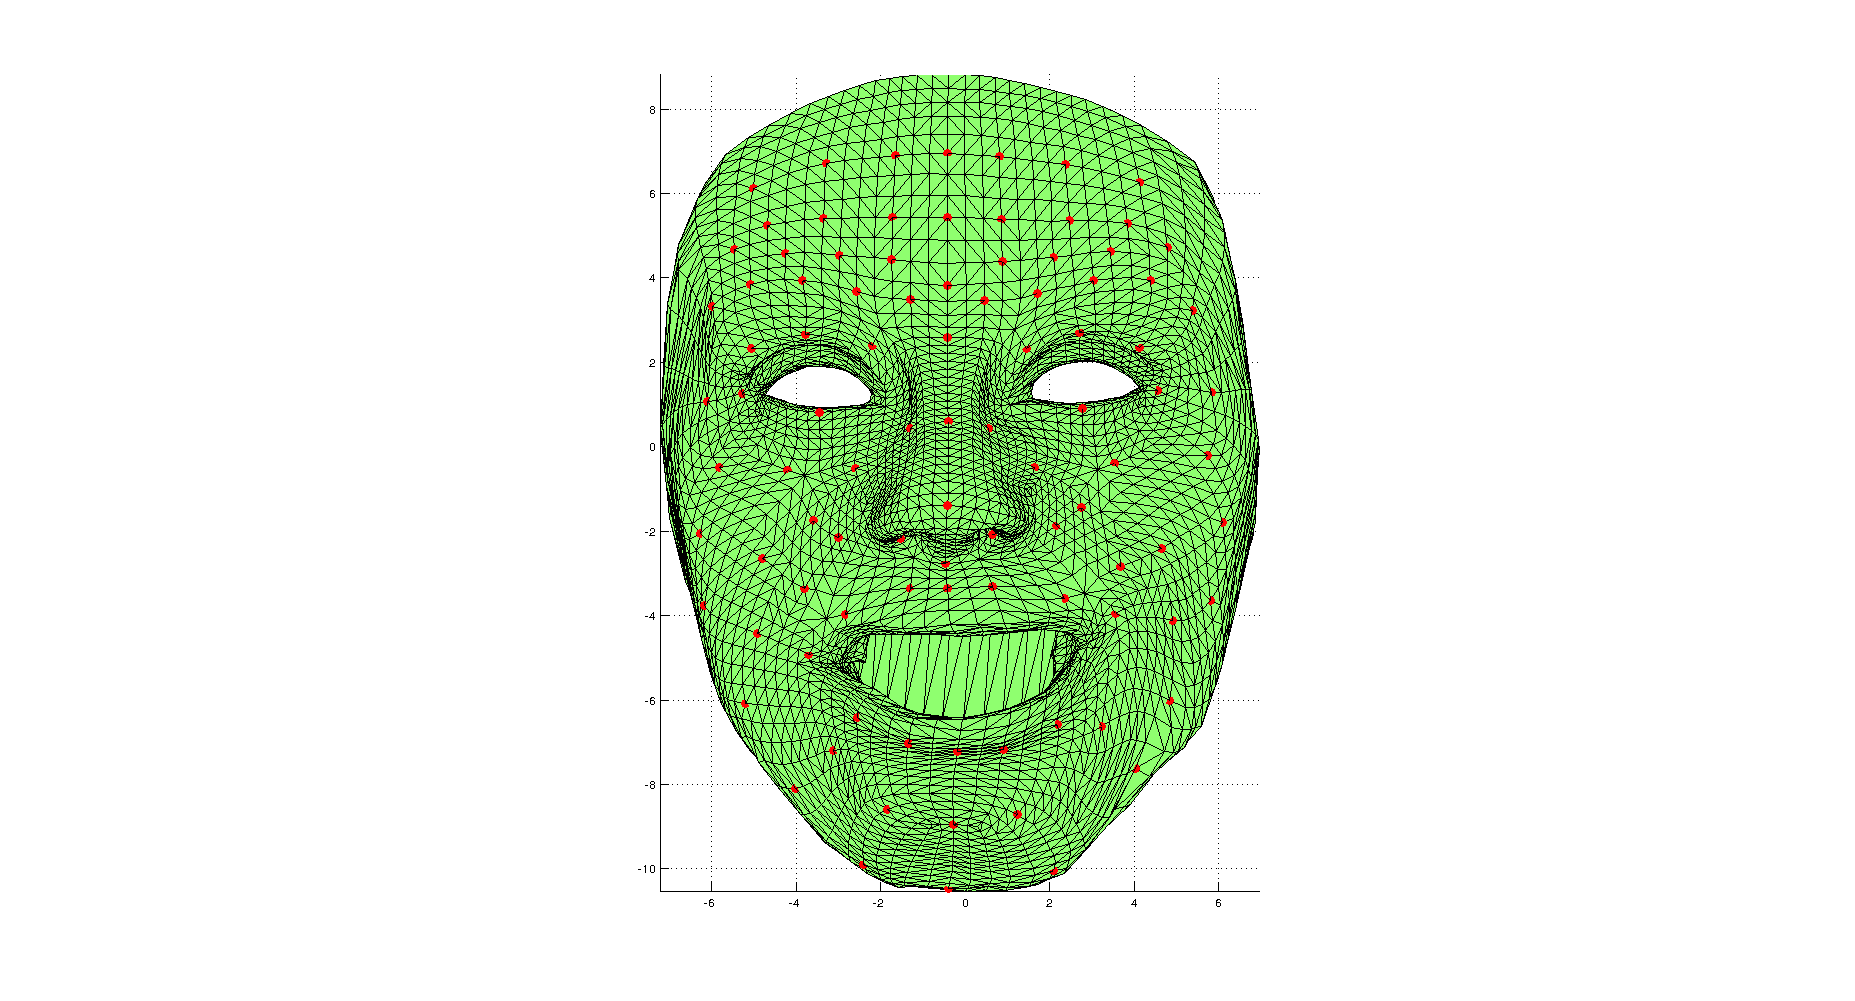
\includegraphics[trim = 160mm 20mm 160mm 10mm,clip,width=0.7\textwidth]{img/weights/3D/Emily_marked/blendshapeE_marked_56.png} 
        \end{subfigure} \\
        \begin{subfigure}[b]{0.25\textwidth}
                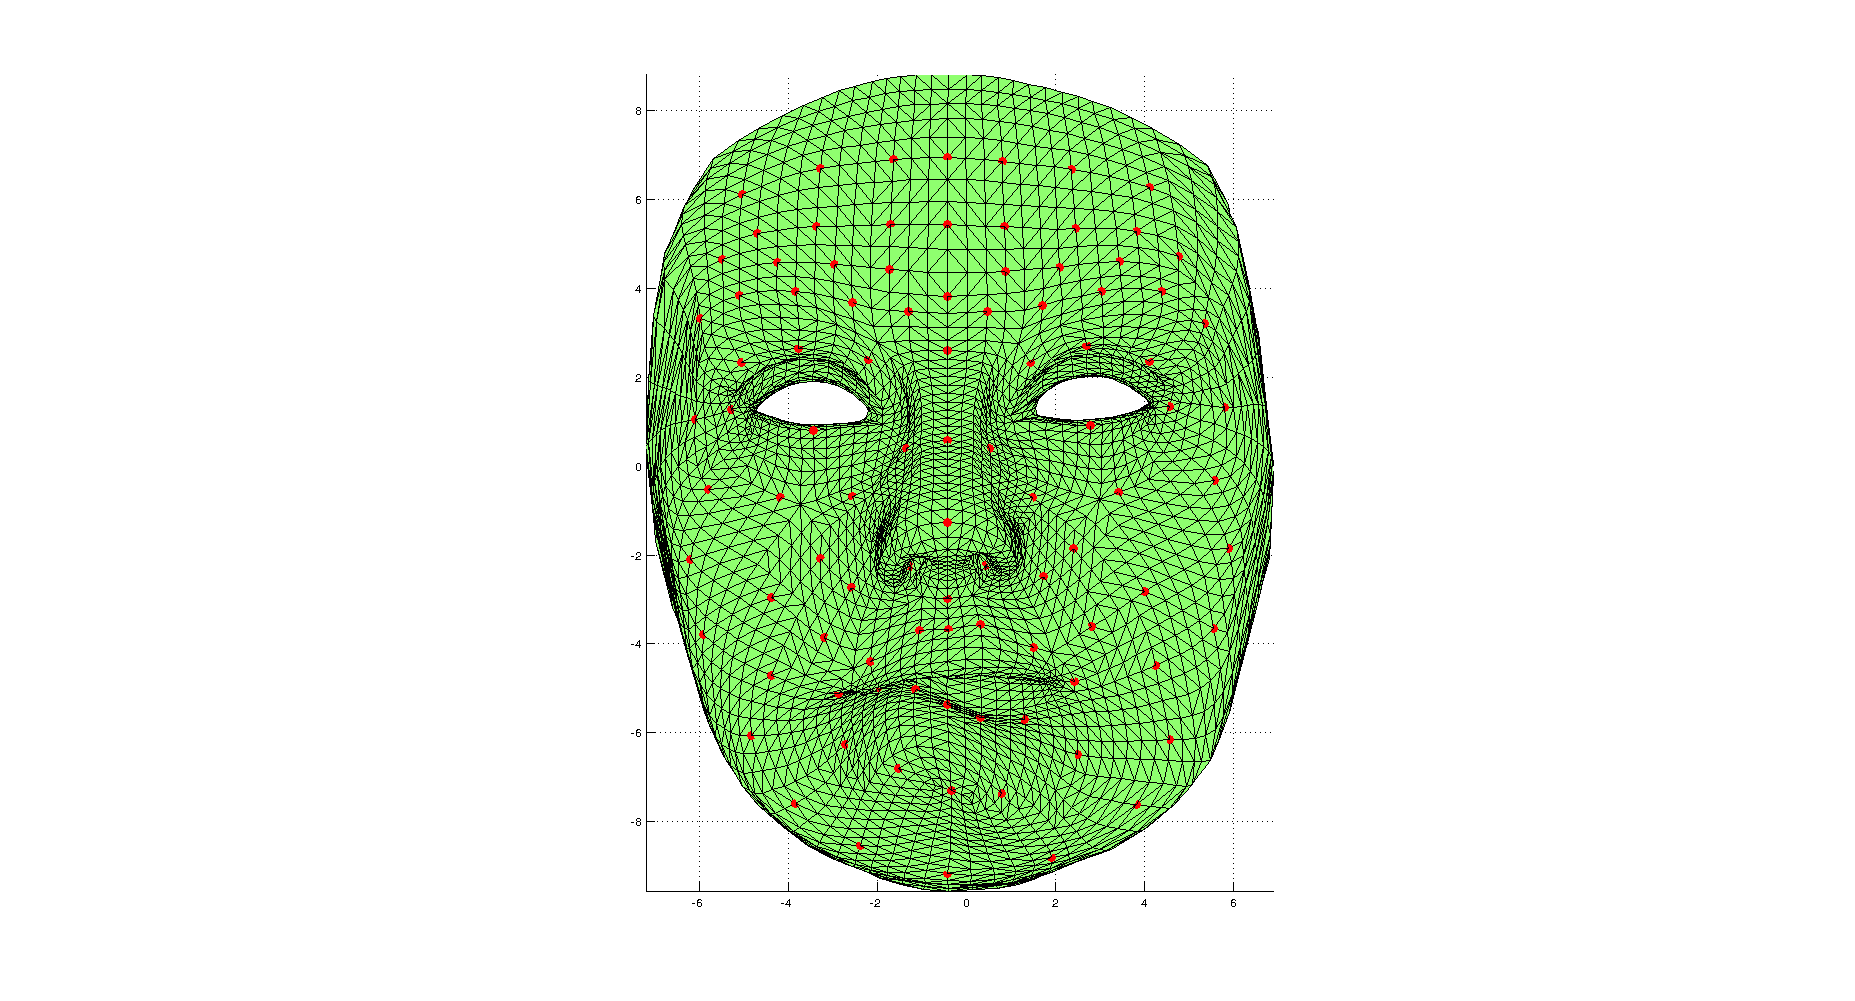
\includegraphics[trim = 160mm 20mm 160mm 10mm,clip,width=0.7\textwidth]{img/weights/3D/Emily_marked/blendshapeE_marked_61.png}
        \end{subfigure}%
        ~ %add desired spacing between images, e. g. ~, \quad, \qquad, \hfill etc.
          %(or a blank line to force the subfigure onto a new line)
        \begin{subfigure}[b]{0.25\textwidth}
                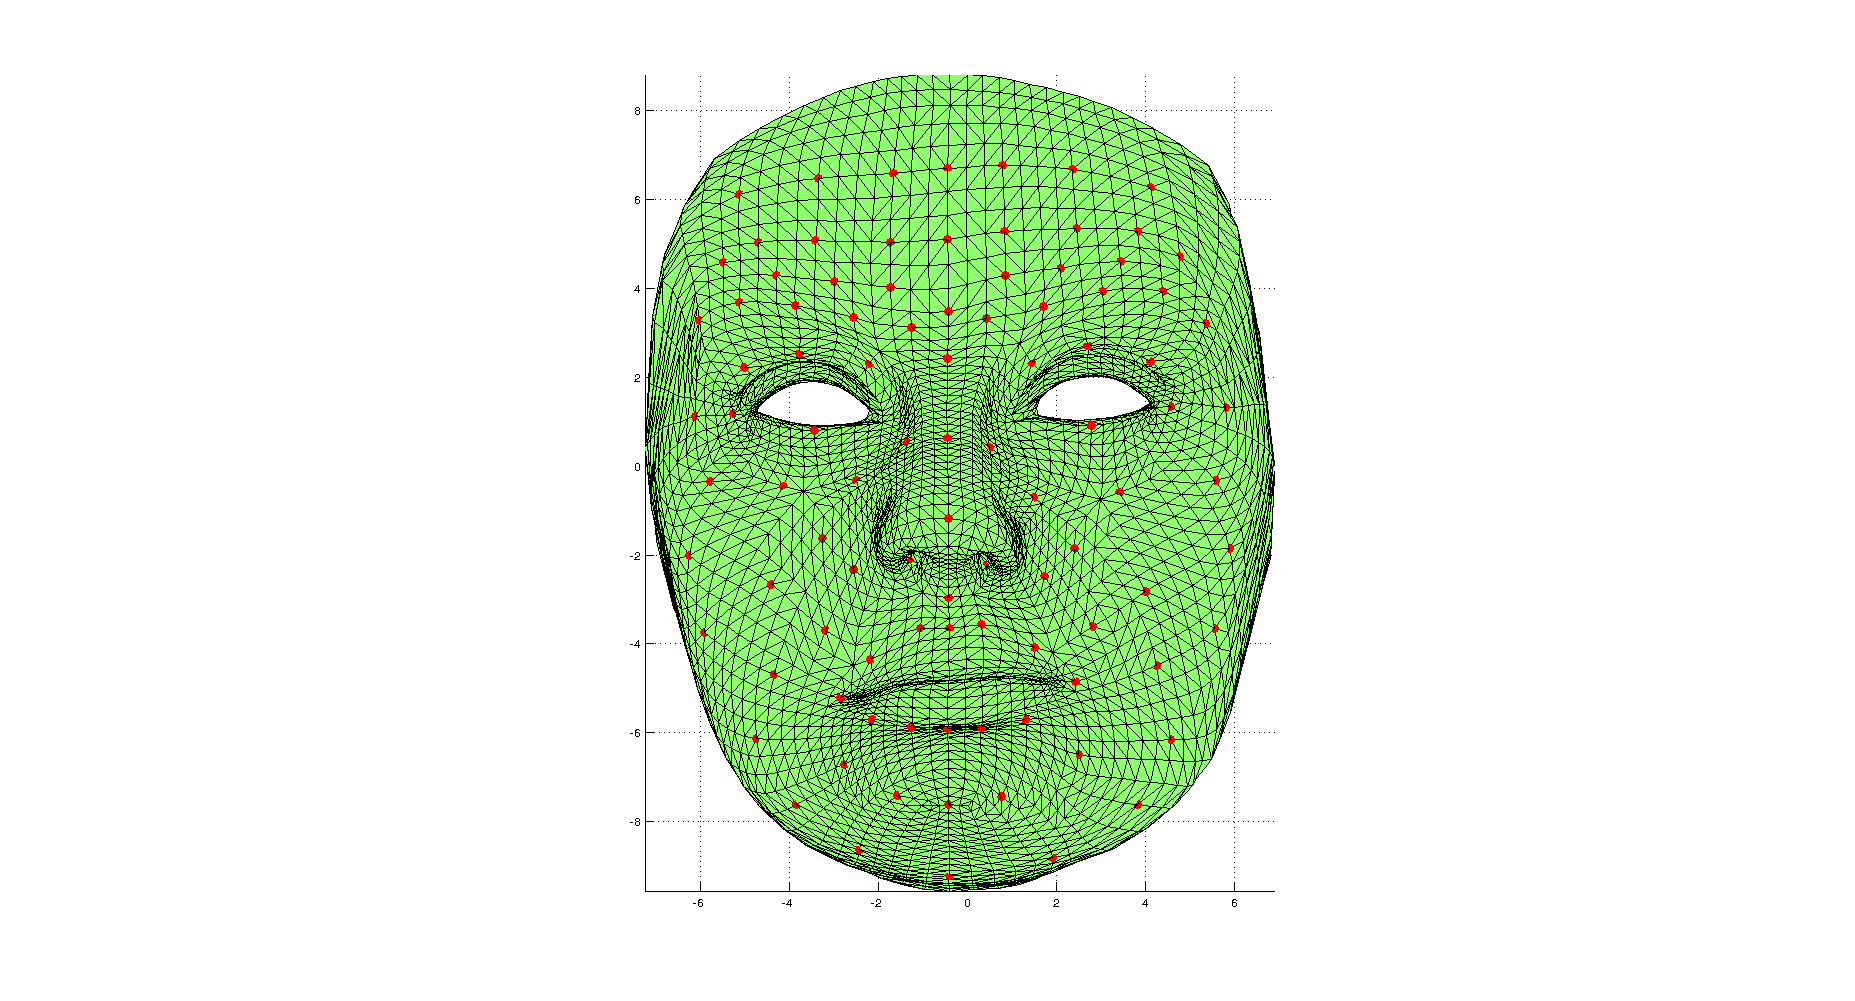
\includegraphics[trim = 160mm 20mm 160mm 10mm,clip,width=0.7\textwidth]{img/weights/3D/Emily_marked/blendshapeE_marked_67.png}
        \end{subfigure}
        ~ %add desired spacing between images, e. g. ~, \quad, \qquad, \hfill etc.
          %(or a blank line to force the subfigure onto a new line)
        \begin{subfigure}[b]{0.25\textwidth}
                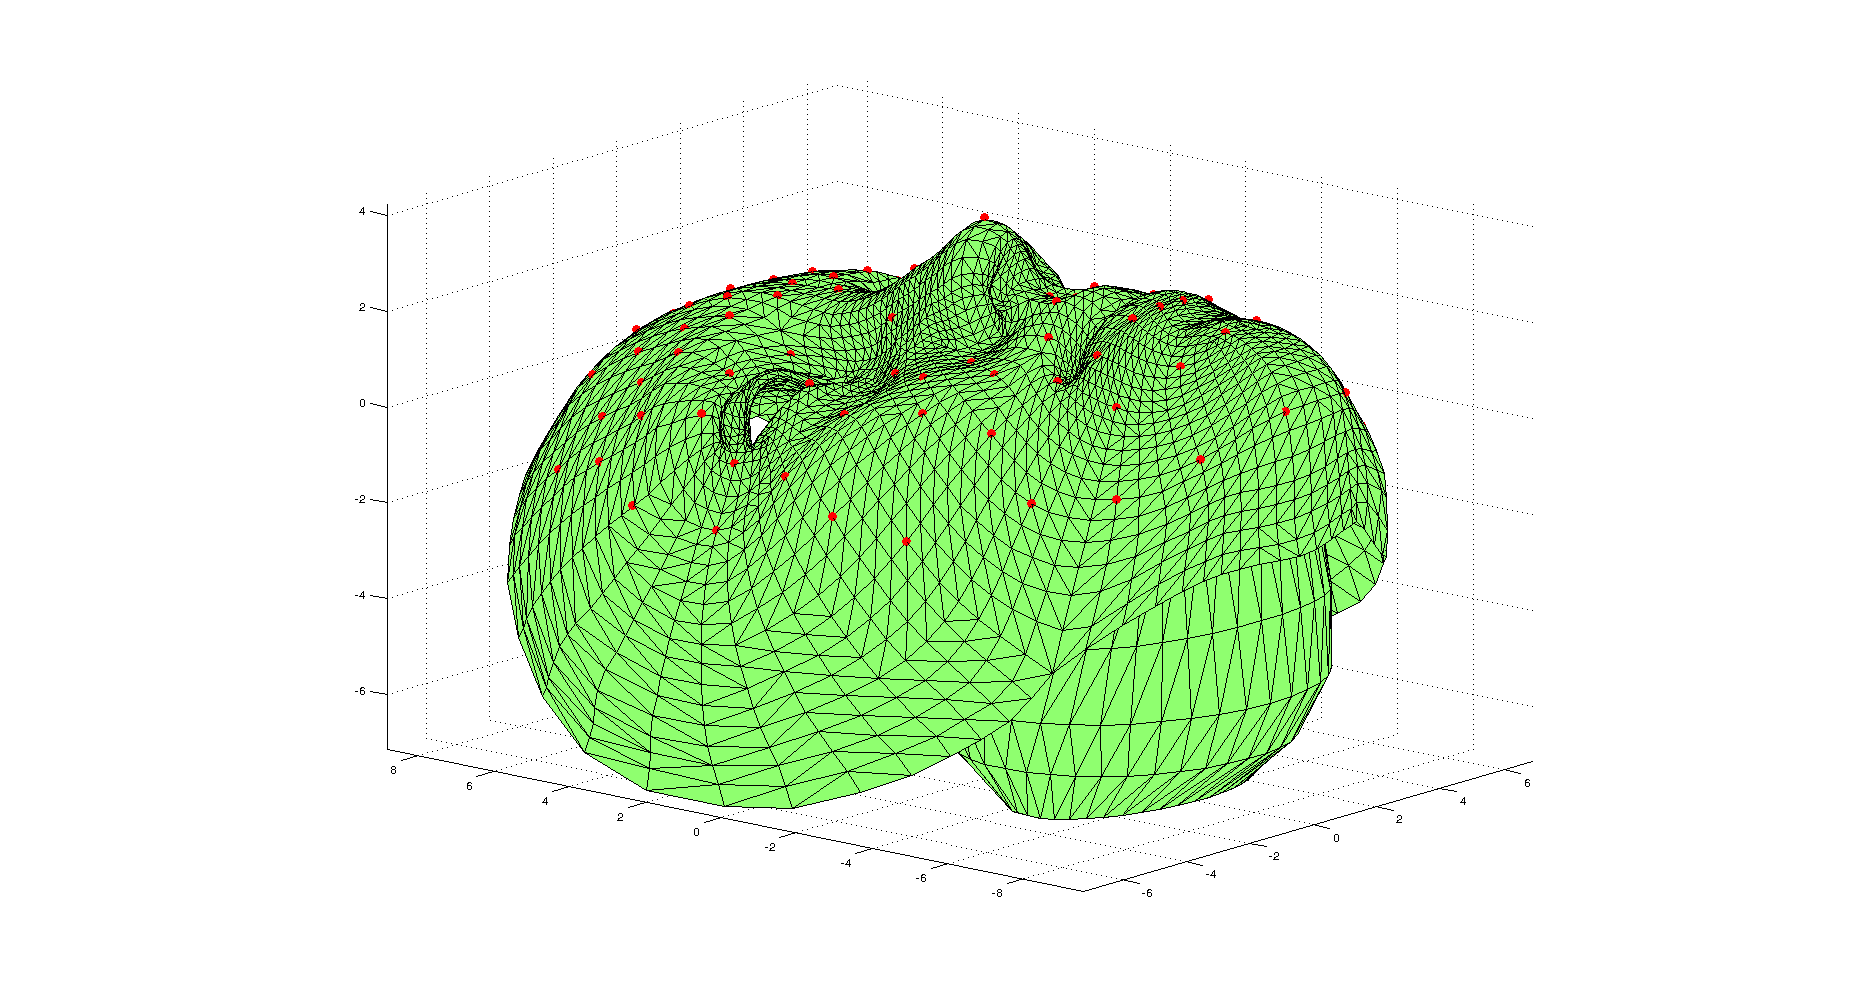
\includegraphics[trim = 120mm 20mm 120mm 10mm, clip, width=0.7\textwidth]{img/weights/3D/Emily_marked/neutralE_marked_rot.png}
        \end{subfigure}
        \caption{Examples of marked blendshapes.}\label{fig:Emarked}
\end{figure}

\begin{figure}[htbp!]
        \centering
        \begin{subfigure}[b]{0.3\textwidth}
                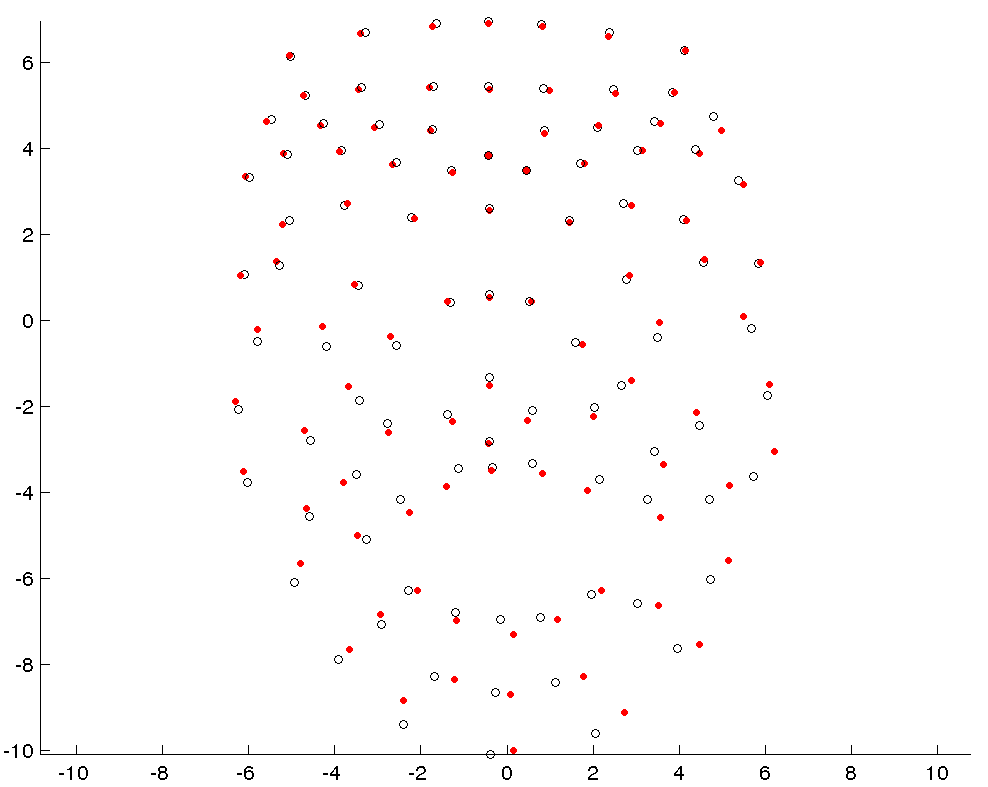
\includegraphics[width=\textwidth]{img/weights/3D/w2/w2_frame200_blends68.png}
        \end{subfigure}%
        ~ %add desired spacing between images, e. g. ~, \quad, \qquad, \hfill etc.
          %(or a blank line to force the subfigure onto a new line)
        \begin{subfigure}[b]{0.3\textwidth}
                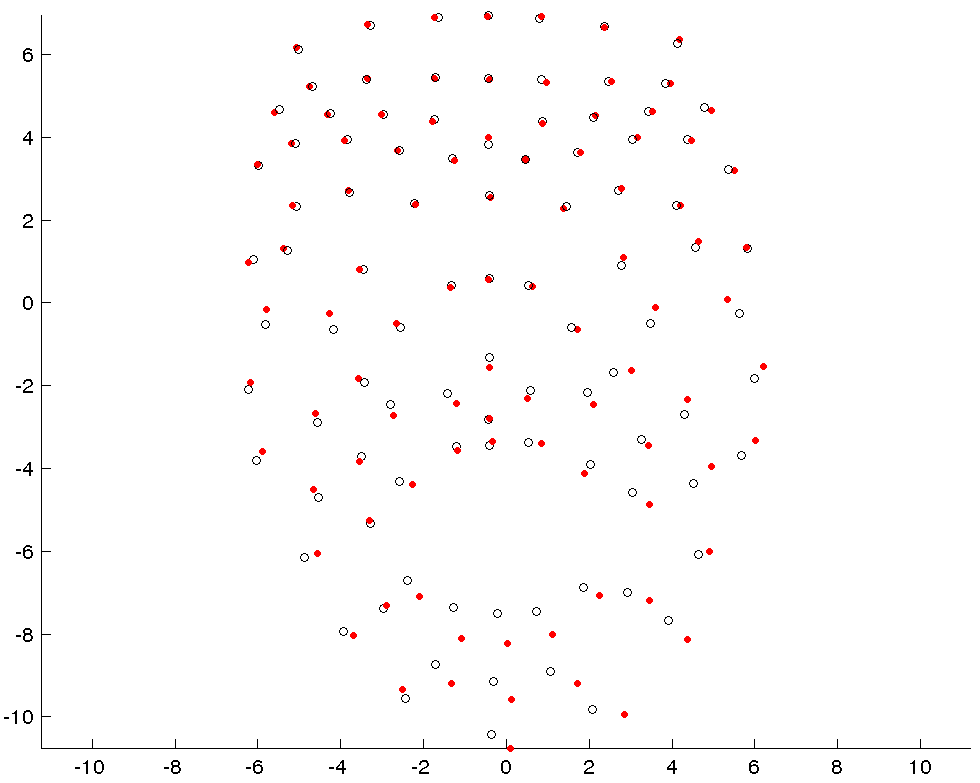
\includegraphics[width=\textwidth]{img/weights/3D/w2/w2_frame400_blends68.png}
        \end{subfigure}
        ~ %add desired spacing between images, e. g. ~, \quad, \qquad, \hfill etc.
          %(or a blank line to force the subfigure onto a new line)
        \begin{subfigure}[b]{0.3\textwidth}
                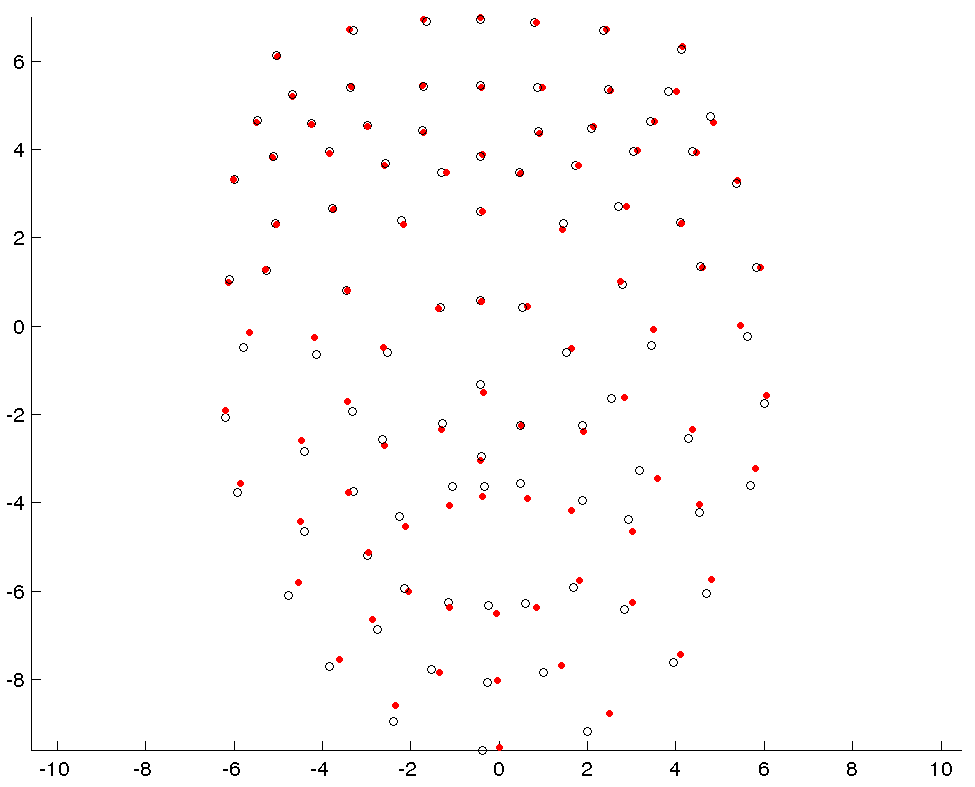
\includegraphics[width=\textwidth]{img/weights/3D/w2/w2_frame600_blends68.png} 
        \end{subfigure} \\
                \begin{subfigure}[b]{0.3\textwidth}
                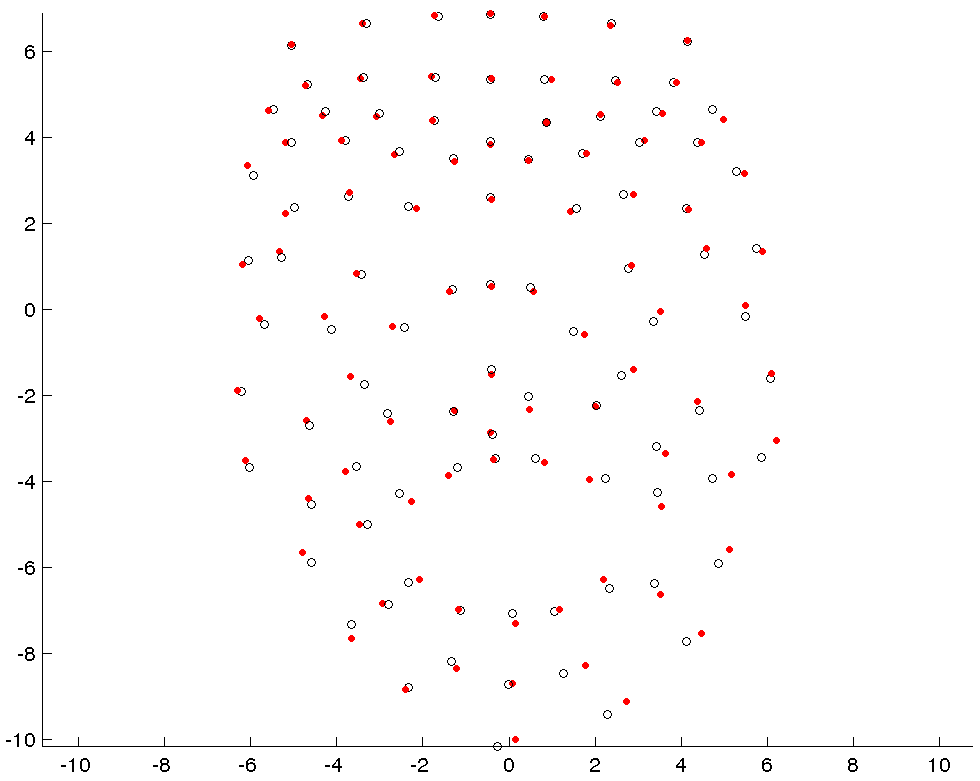
\includegraphics[width=\textwidth]{img/weights/3D/w3/w3_200.png}
        \end{subfigure}%
        ~ %add desired spacing between images, e. g. ~, \quad, \qquad, \hfill etc.
          %(or a blank line to force the subfigure onto a new line)
        \begin{subfigure}[b]{0.3\textwidth}
                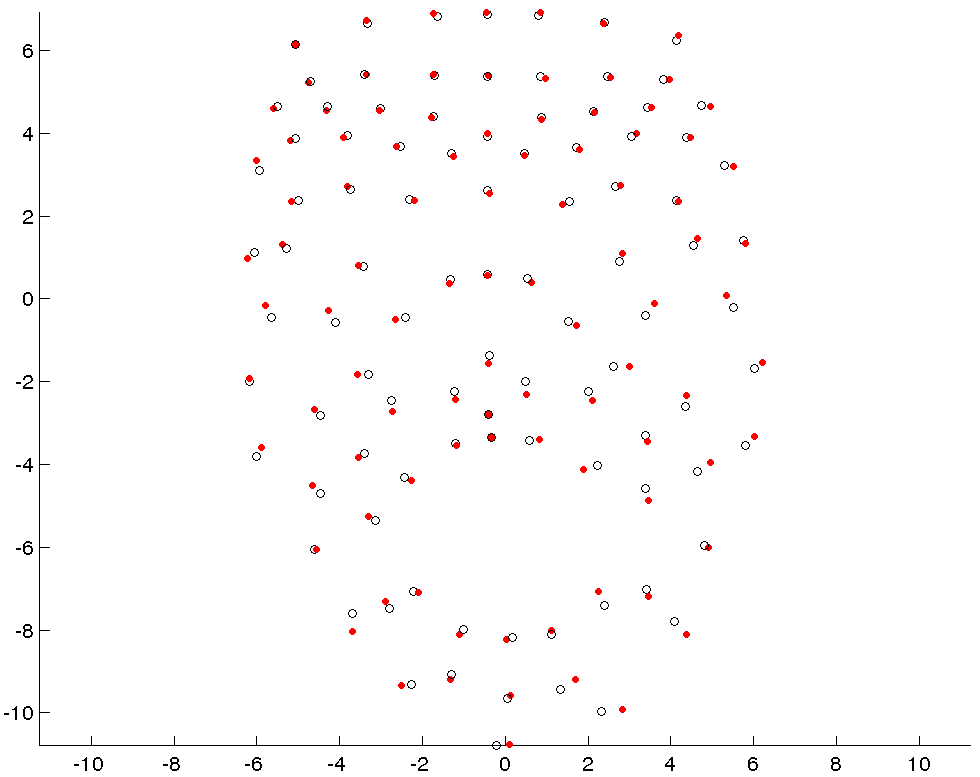
\includegraphics[width=\textwidth]{img/weights/3D/w3/w3_400.png}
        \end{subfigure}
        ~ %add desired spacing between images, e. g. ~, \quad, \qquad, \hfill etc.
          %(or a blank line to force the subfigure onto a new line)
        \begin{subfigure}[b]{0.3\textwidth}
                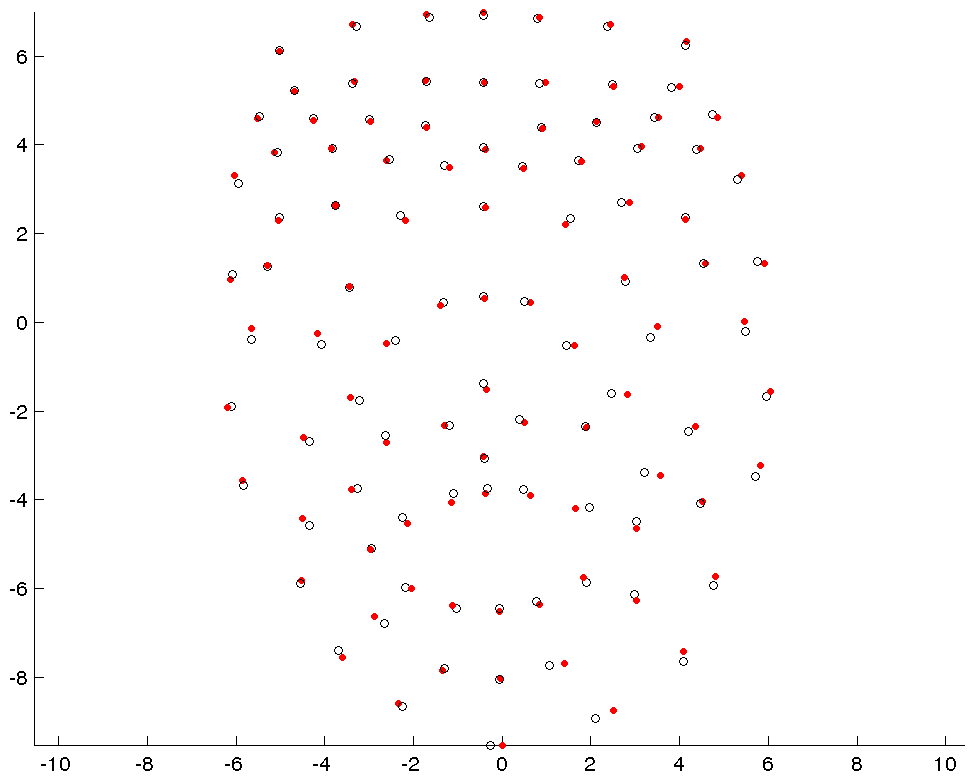
\includegraphics[width=\textwidth]{img/weights/3D/w3/w3_600.png} 
        \end{subfigure}
        \caption{The red dots mark the position of the markers in the motion sequence while the black cirles correspond to the reconstructed position of the markers. The top results were produced using the non-negative least-squares solver while the bottom results were produced by the linear least-squares solver. }\label{fig:errorw2w3}
\end{figure}

The use of blendshapes greatly improves the visual quality of the resulting animation. However, the animation still lacks realism and expressiveness, thus we implement a number of changes to the original model. Firstly, we aim to find a sparse solution, i.e. minimise the number of blendshapes used at any given time. This is done by adding a penalty term on the $L1$-norm of the weights to the original minimisation problem. Then an iterative method is used to find the optimal set of weights; we use a Matlab implementation of the LASSO algorithm~\cite{Schmidt:2005}. After careful adjustment of the scaling parameter, the least squares solver is able to reduce the mean reconstruction error by approximately $0.03$ centimetres. However, the best sparse results were achieved without imposing the upper and lower bound on the weights. We found that in our case it is more import to impose these bounds than to favour sparse solutions. Moreover, the solution produced by the constrained non-negative least squares solver uses on average $21$ blendshapes per frame, which does not seem unreasonable given the complexity of human facial motion.

As noted by Bouaziz et al., a motion capture sequence also has temporal constraints, i.e. each frame is closely related to the previous frames~\cite{Bouaziz:2013}. This constraint may be included in the minimisation problem by adding a smoothness term, $||\w^{t-2} - 2 \w^{t-1} + \w^t||^2_2$, where $\w$ is the vector of weights, and $t$ is the frame number. The resulting problem is generally hard to solve, but there exist a number of algorithms that minimise the sum of Euclidean norms. Beside the one mention in the paper by Bouaziz et al., we have considered the algorithms proposed by Andersen et al., and Xue and Ye~\cite{Andersen:2000}, ~\cite{Xue:1997}. However, after examining the solution produced by our current methods, we noticed that it automatically obeys this smoothness constraint; this may be explained by the fact that the input sequence was filmed at a relatively high frame rate ($60$ frames per second). Specifically, we compared the change in blendshape weights from frame to frame; the average difference is $0.007$, which, when reconstructed, is hardy noticeable. The highest differences (of around $0.3$) appear during the opening and closing of the mouth; these transitions look natural at the original frame rate. We note that if the motion capture data was recorded at a low frame rate, then the implementation of the temporal constraints might improve the quality of the resulting animation.

Next, we examined the effect of using a reduced set of key expressions in the solver; this leads to a smaller system of equations to be optimised. The reduced set contains $19$ shapes included in the visual set of controls in the original blendshape model. The smaller set of shapes leads to a slight increase (of approximately $0.03$ centimetres) in reconstruction error. There is no noticeable effect on the visual quality of the resulting animation, see Fig.~\ref{fig:19blends}. Thus the only notable advantage of using fewer blendshapes is the acceleration of the  optimisation step. However, if the performance of the algorithm is the main objective, then a PCA basis is a better choice than a reduced non-orthogonal set of shapes.

\begin{figure}[htbp!]
        \centering
        \begin{subfigure}[b]{0.3\textwidth}
                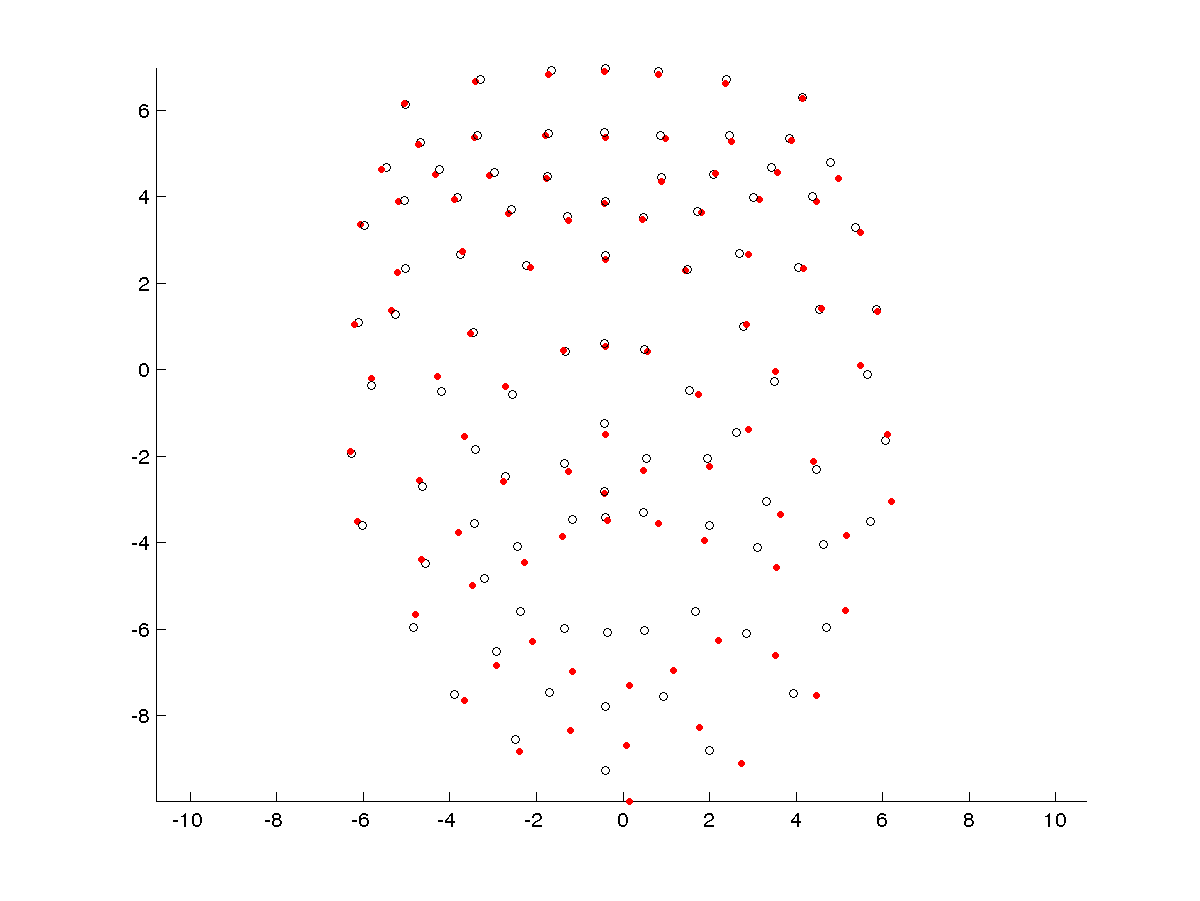
\includegraphics[trim = 10mm 0mm 10mm 0mm,clip,width=\textwidth]{img/weights/3D/19blends/w2_frame200_blends19.png}
        \end{subfigure}%
        ~ %add desired spacing between images, e. g. ~, \quad, \qquad, \hfill etc.
          %(or a blank line to force the subfigure onto a new line)
        \begin{subfigure}[b]{0.3\textwidth}
                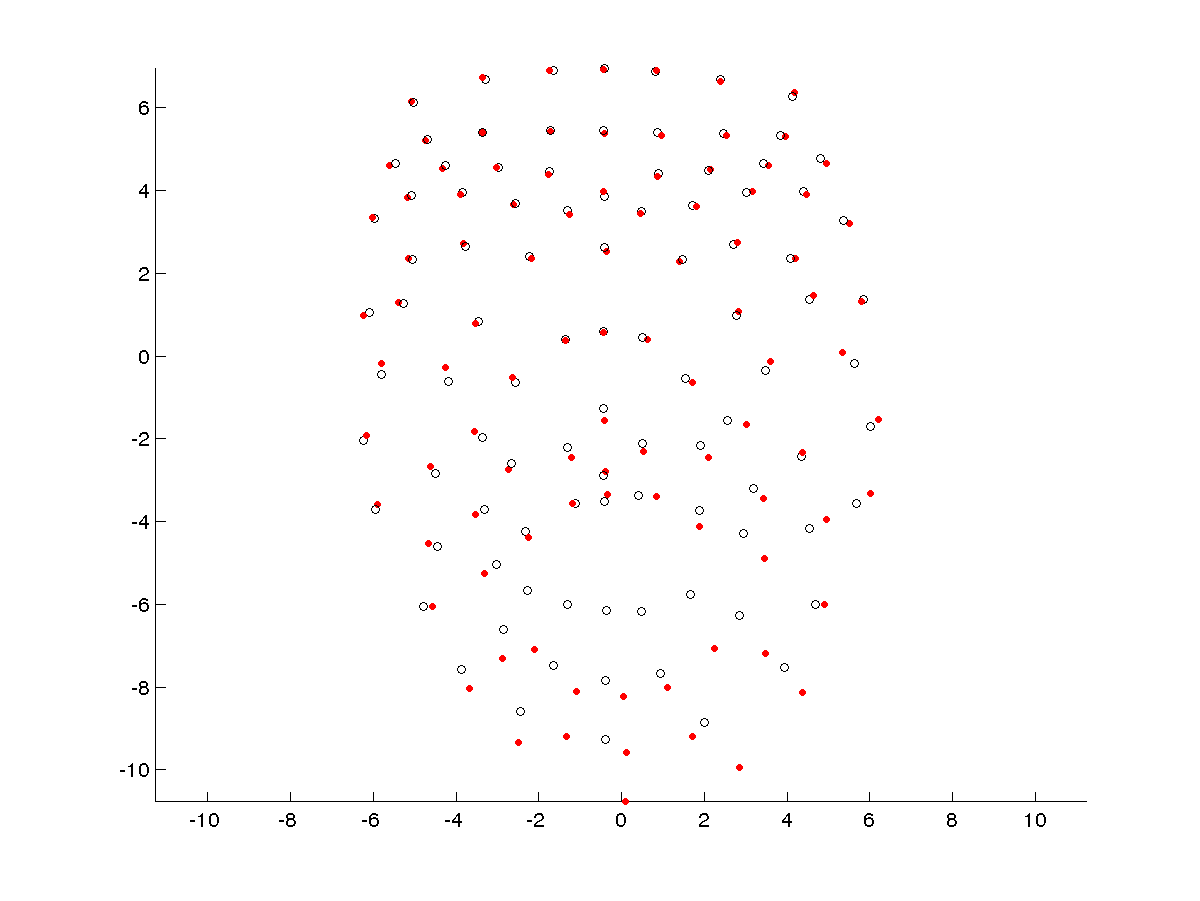
\includegraphics[trim = 10mm 0mm 10mm 0mm,clip,width=\textwidth]{img/weights/3D/19blends/w2_frame400_blends19.png}
        \end{subfigure}
        ~ %add desired spacing between images, e. g. ~, \quad, \qquad, \hfill etc.
          %(or a blank line to force the subfigure onto a new line)
        \begin{subfigure}[b]{0.3\textwidth}
                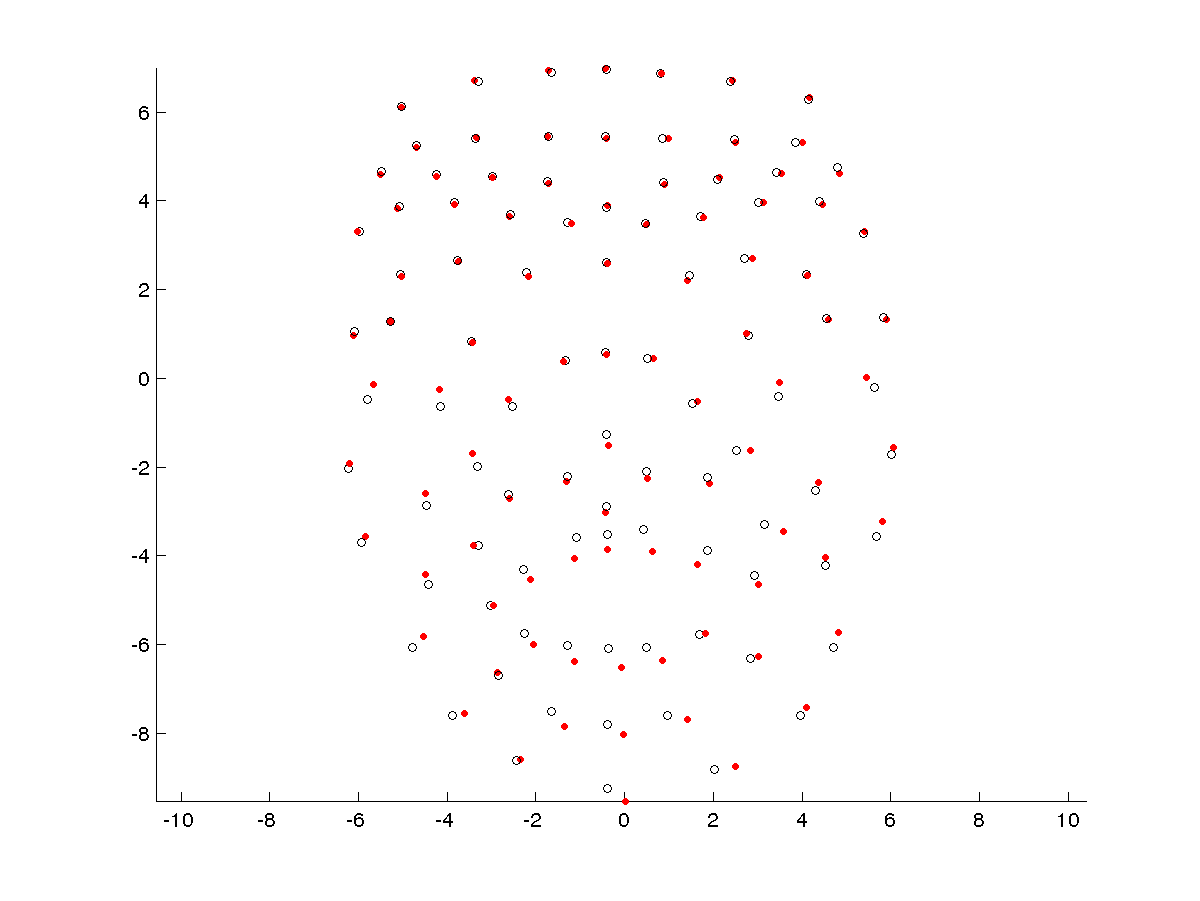
\includegraphics[trim = 10mm 0mm 10mm 0mm,clip,width=\textwidth]{img/weights/3D/19blends/w2_frame600_blends19.png} 
        \end{subfigure} \\
        \begin{subfigure}[b]{0.3\textwidth}
                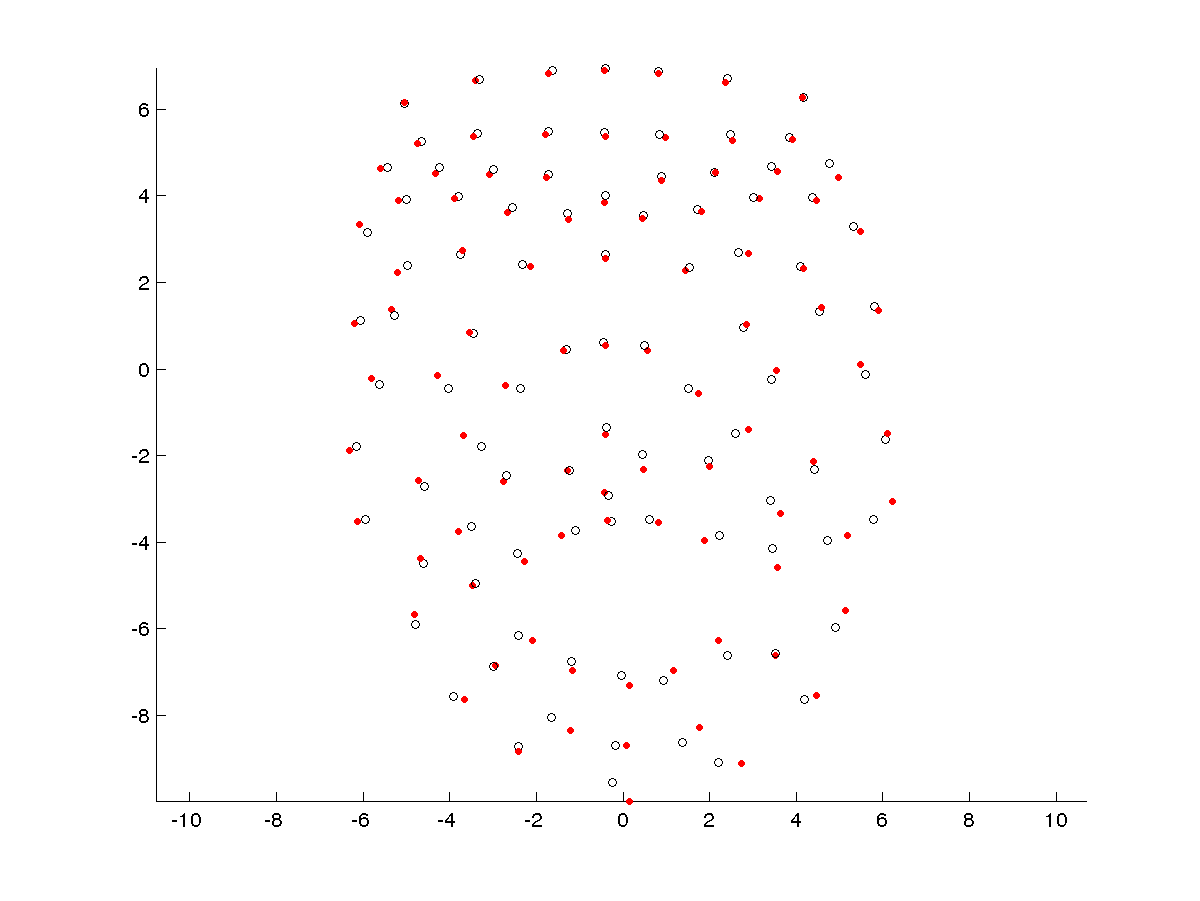
\includegraphics[trim = 10mm 0mm 10mm 0mm,clip,width=\textwidth]{img/weights/3D/19blends/w3_frame200_blends19.png}
        \end{subfigure}%
        ~ %add desired spacing between images, e. g. ~, \quad, \qquad, \hfill etc.
          %(or a blank line to force the subfigure onto a new line)
        \begin{subfigure}[b]{0.3\textwidth}
                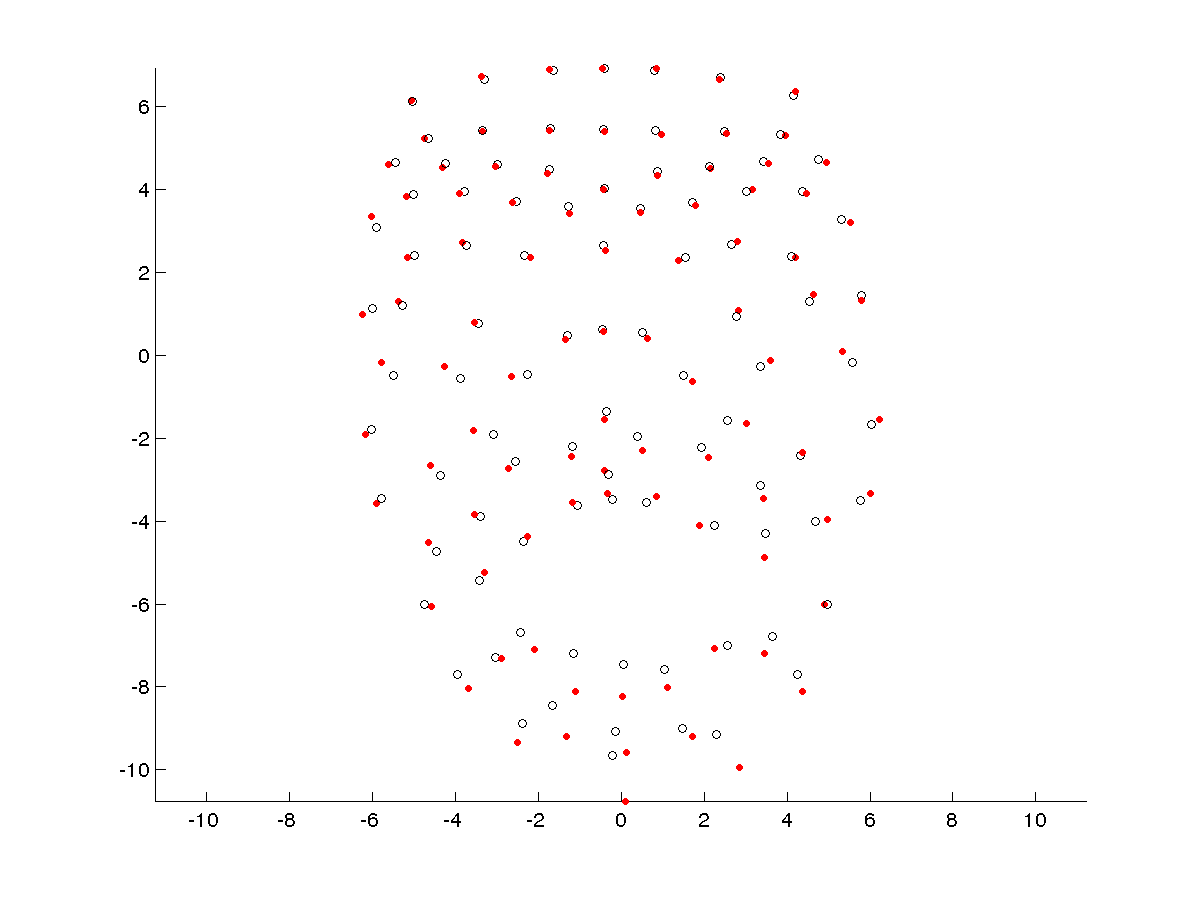
\includegraphics[trim = 10mm 0mm 10mm 0mm,clip,width=\textwidth]{img/weights/3D/19blends/w3_frame400_blends19.png}
        \end{subfigure}
        ~ %add desired spacing between images, e. g. ~, \quad, \qquad, \hfill etc.
          %(or a blank line to force the subfigure onto a new line)
        \begin{subfigure}[b]{0.3\textwidth}
                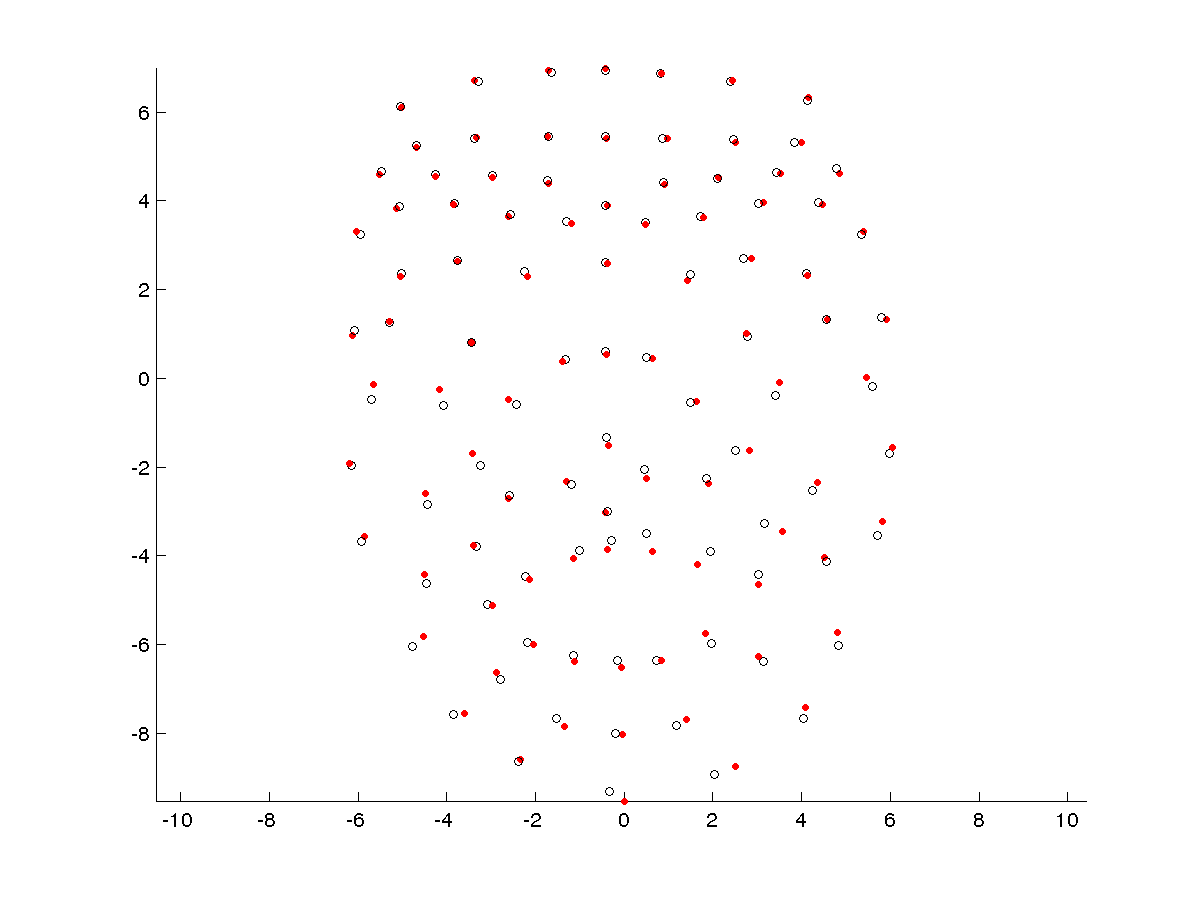
\includegraphics[trim = 10mm 0mm 10mm 0mm,clip,width=\textwidth]{img/weights/3D/19blends/w3_frame600_blends19.png} 
        \end{subfigure}
        \caption{The reconstruction error for a model with $19$ blendshapes. The top results were produced using the non-negative least-squares solver while the bottom results were produced by the linear least-squares solver. Colours as in Fig.~\ref{fig:errorw2w3}.}\label{fig:19blends}
\end{figure}

For comparison, we attempt the opposite approach; we include extra blendshapes to account for the features that are not present in the original set. This approach was inspired by the research of Li et al., who introduced corrective shapes to systematically extend the initial set of shapes~\cite{Li:2013}. The authors start by using linear combinations of PCA principal components to construct new facial expressions. They then extract a number of samples that cannot be explained by the original set of principal components. An iterative procedure is used to produce corrective shapes that are orthogonal to the members of the original set, and that improve the fitting accuracy. Unfortunately, such corrective method cannot be applied to a manually constructed set of blendshapes since it relies on vector orthogonality. Instead, we manually construct a set of new shapes that are more extreme than our original blendshapes; we then include these new shapes in the solver. The criteria for choosing the new expressions are, (a) the likelihood of that or similar expressions, and (b) the dissimilarity of the new expressions in comparison to the existing ones. The four extra blendshapes are shown in Fig.~\ref{fig:extrafaces}; they were constructed by increasing the weights on the original blendshapes beyond the predefined limit. 
\begin{figure}[htbp!]
        \centering
        \begin{subfigure}[b]{0.23\textwidth}
                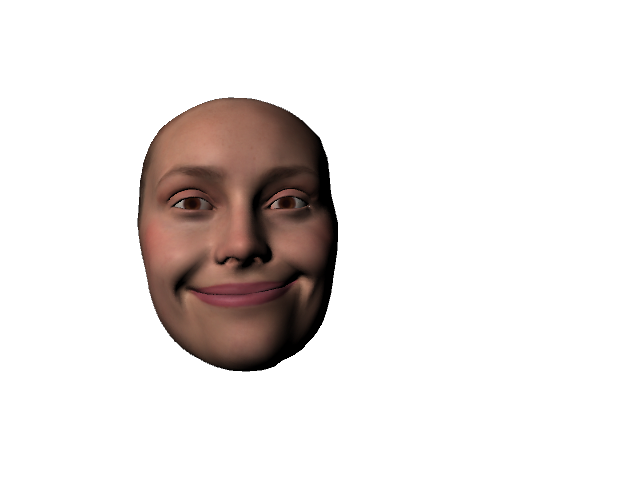
\includegraphics[trim = 50mm 30mm 80mm 30mm,clip,width=\textwidth]{img/weights/3D/Extrafaces/lipcorners15.png}
        \end{subfigure}
        ~ %add desired spacing between images, e. g. ~, \quad, \qquad, \hfill etc.
          %(or a blank line to force the subfigure onto a new line)
        \begin{subfigure}[b]{0.23\textwidth}
                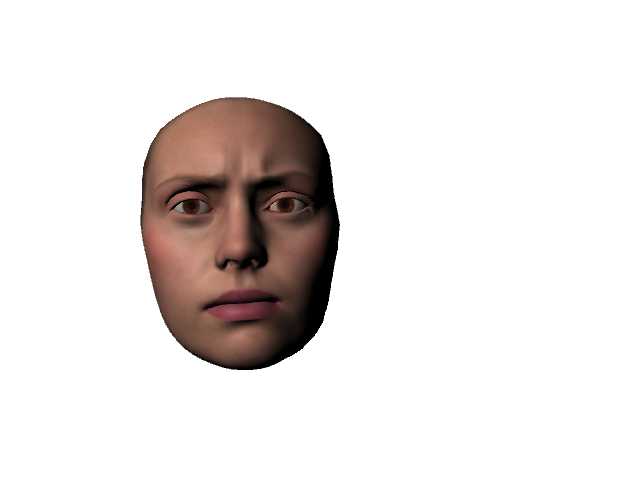
\includegraphics[trim = 50mm 30mm 80mm 30mm,clip,width=\textwidth]{img/weights/3D/Extrafaces/eyebrowsin2.png}
        \end{subfigure} 
        \begin{subfigure}[b]{0.23\textwidth}
                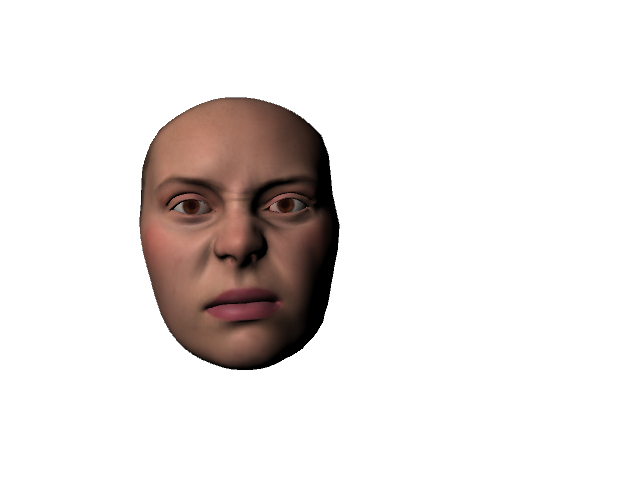
\includegraphics[trim = 50mm 30mm 80mm 30mm,clip,width=\textwidth]{img/weights/3D/Extrafaces/nosewrinkle2.png}
        \end{subfigure}
        ~ %add desired spacing between images, e. g. ~, \quad, \qquad, \hfill etc.
          %(or a blank line to force the subfigure onto a new line)
        \begin{subfigure}[b]{0.23\textwidth}
                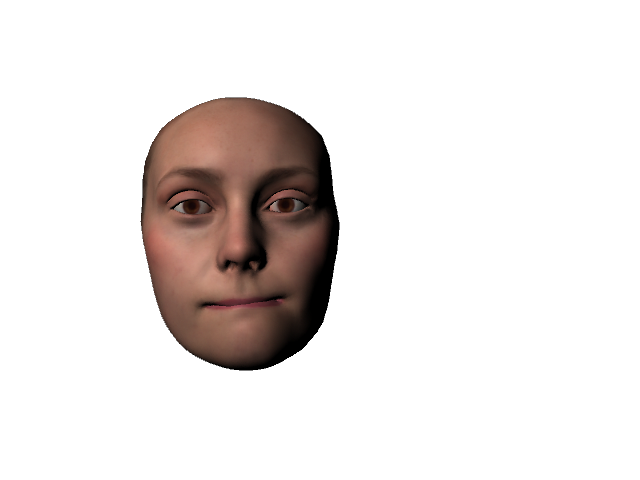
\includegraphics[trim = 50mm 30mm 80mm 30mm,clip,width=\textwidth]{img/weights/3D/Extrafaces/mouthsuck.png}
        \end{subfigure}
        \caption{Additional blendshapes. }\label{fig:extrafaces}
\end{figure}
\begin{figure}[htbp!]
        \centering
        \begin{subfigure}[b]{0.47\textwidth}
                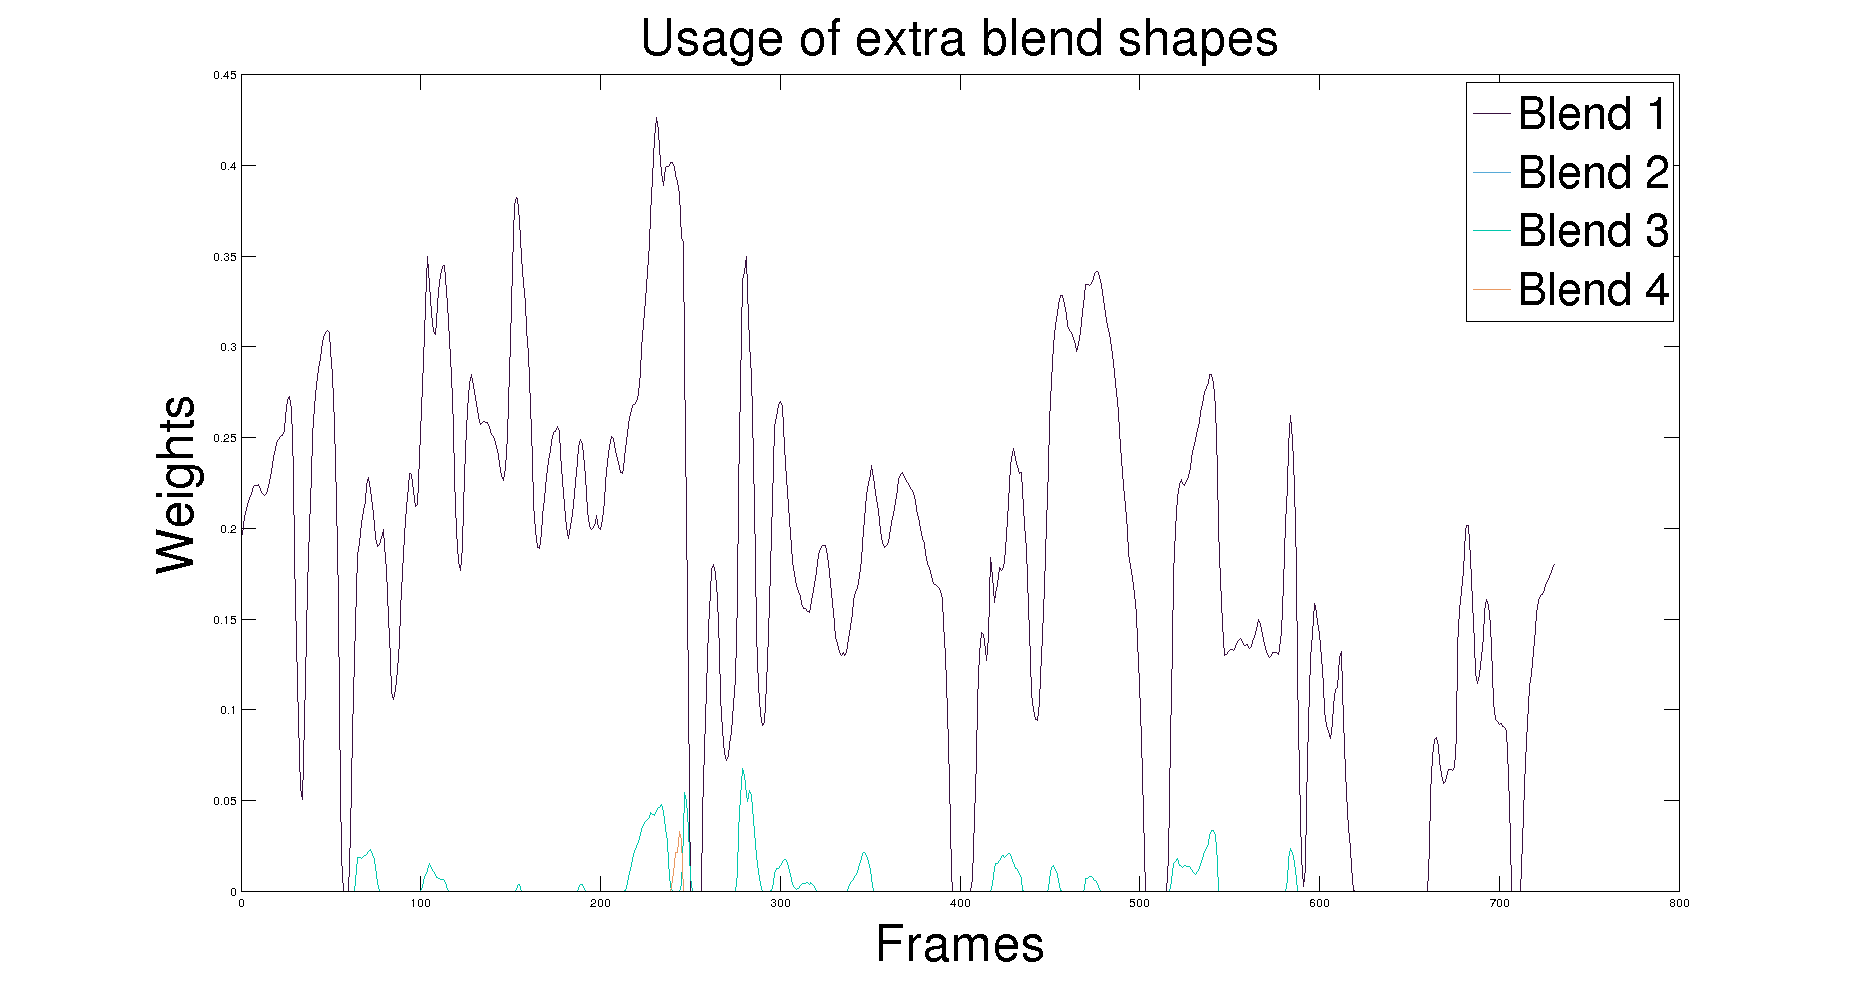
\includegraphics[trim = 10mm 0mm 10mm 0mm,clip,width=\textwidth]{img/weights/3D/Extrafaces/w2_72_usage.png}
        \end{subfigure}
        ~ %add desired spacing between images, e. g. ~, \quad, \qquad, \hfill etc.
          %(or a blank line to force the subfigure onto a new line)
        \begin{subfigure}[b]{0.47\textwidth}
                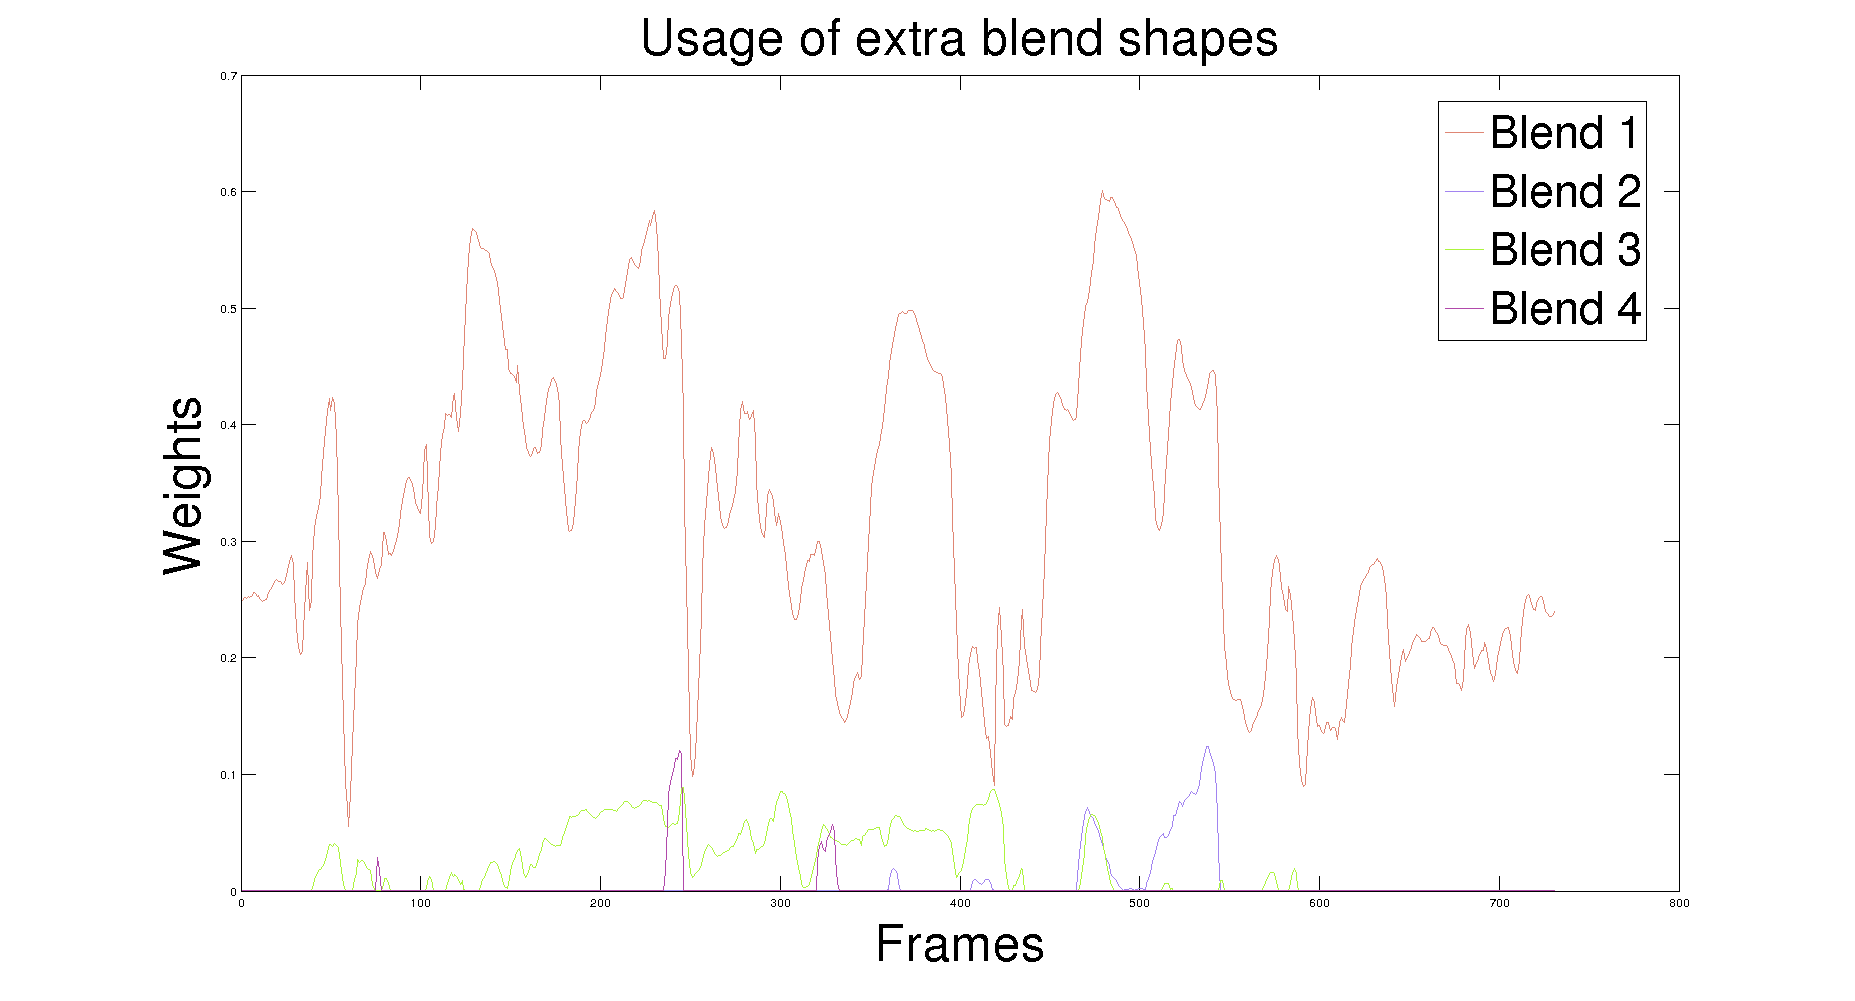
\includegraphics[trim = 10mm 0mm 10mm 0mm,clip,width=\textwidth]{img/weights/3D/Extrafaces/w3_72_usage.png}
        \end{subfigure}
        \caption{The weights associated with the extra blendshapes as a function of frames in the sequence. The left diagram corresponds to the constrained non-negative least-squares solver while the right one gives he results for the linear least-squares solver.}\label{fig:usage}
\end{figure}
Fig.~\ref{fig:usage} shows the activation of the extra blendshapes throughout the motion sequence. Both of the optimisation methods favour the first additional blendshape that corresponds to the smile in Fig.~\ref{fig:extrafaces} while the other shapes are only used with low weights. Despite the extension to the set of shapes, the reconstruction error decreased by less then $0.01$ centimetres for both methods. This is explained by the fact that the extra blenshapes are closely related to the original ones, as they are in fact a linear combination of the original blendshapes. A more systematic approach needs to be used to produce more diverse shapes. For example, an additional optimisation step may be included that randomly alters the existing blendshapes, and uses a small subset of the altered shapes to find the extension of the blendshape set that minimises the reconstruction error. In particular, we choose a set of new shapes that are constructed by adding a small random quantity to the average of the existing set. Then these shapes are included in the optimisation algorithm. The new shapes are stored if they reduce the reconstruction error, and new blendshapes are suggested until the error decreases below a chosen threshold. Using this iterative procedure, we are able to reduce the reconstruction error by about $10 \%$; however, this approach is very computationally intensive, and the new shapes cannot be easily included in the existing model. 

\subsubsection{Estimation of Weights in Actor's Domain}

At this stage our best results still lack expressiveness and visual appeal. In the current pipeline, we first transform the motion sequence from the actor to Emily, and then solve for the blendshapes in the Emily domain. This approach relies on the transformation to produce valid motion in the Emily domain; however, the transformation is geometrical, and it does not guarantee to produce a realistic and natural-looking animation. Therefore, we test the opposite approach. We first find the thin plate spline transformation $\mathbf{T}$ from the actor's neutral expression to Emily's neutral expression. Then the inverse transformation $\mathbf{T^{-1}}$ is used to map the Emily blendshapes to the actor's domain. We thus have matching sets of sparse blendshapes in both domains, see Fig~\ref{fig:EtoR}. The weights are calculated at each frame using the original captured sequence and the newly designed blendshapes in the actor's domain; these weights are then applied directly in the Emily domain. 

\begin{figure}[htbp!]
        \centering
        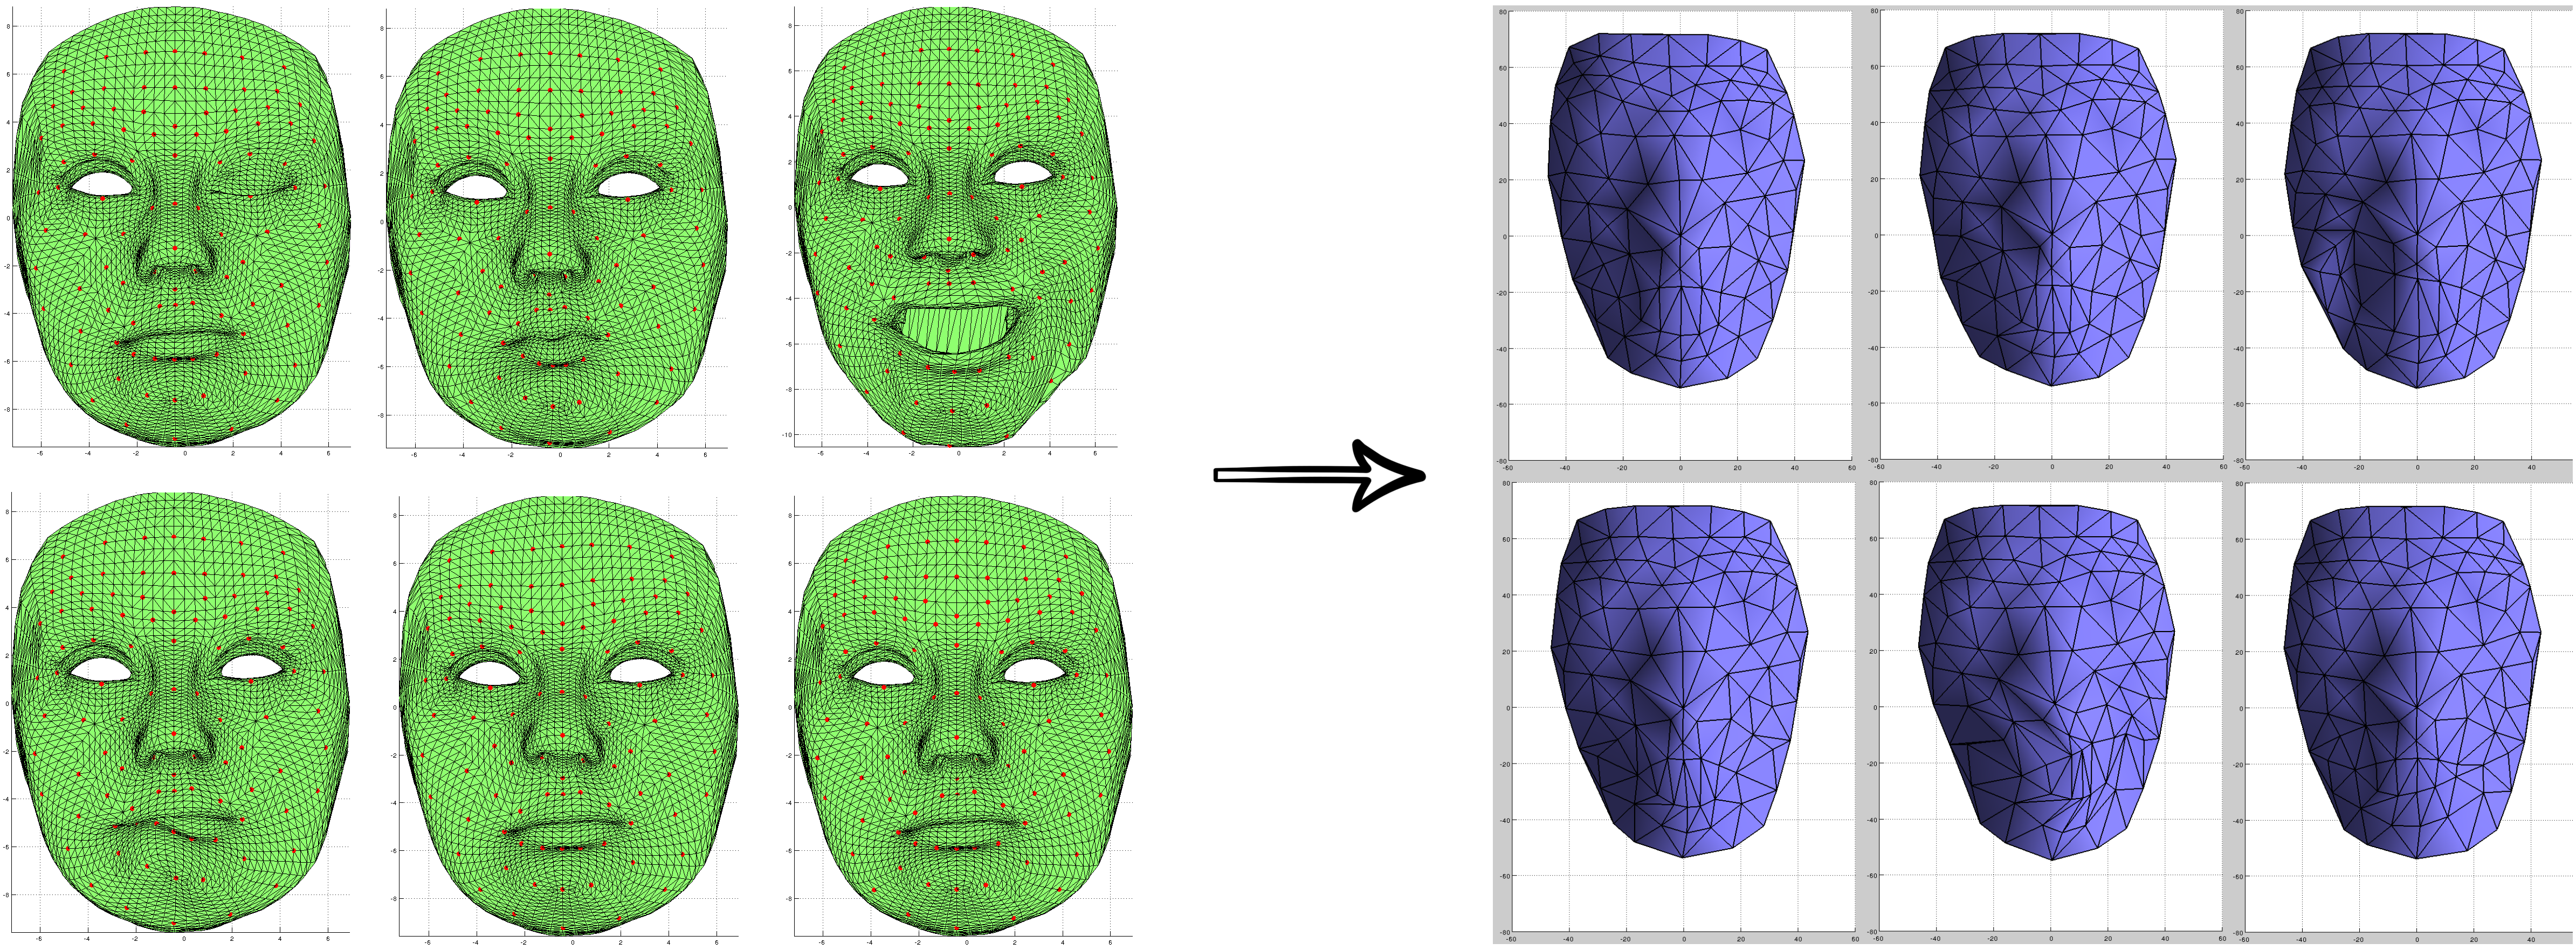
\includegraphics[width=0.8\textwidth]{img/EtoRblends}
        \caption{Use the inverse thin plate spline transform $\mathbf{T^{-1}}$ to produce a set of blendshapes in the actor's domain. The left images are the sparse Emily blendshapes (red dots) while the right images are the sparse actor's blendshapes (vertices of the mesh)}\label{fig:EtoR}
\end{figure}

Fig.~\ref{fig:resultcomp} compares the results produced using the two antipode approaches. The new approach is able to better mimic the motion of the actor, and it improves the appearance of the digital model, i.e. the new animation appears more natural and realistic. Note that the original method tries to reproduce the actor's performance using the transformed geometrical data while the new method relies more on the semantics associated with the blendshapes. In particular, we do not expect the actor and Emily expressions to match identically, for example one of them might be able to raise the eye-brows higher than the other. The new approach is better at respecting and enhancing the different features of the two faces. The mean reconstruction error is smaller than $0.01$ centimeters which is an improvement over the previous methods. We test our new approach using another motion capture sequence; in the new sequence the actor pulls the expressions listed in the Facial Action Coding System~\cite{FACS}. This sequence is more challenging as the expressions are diverse and intricate as opposed to the rather monotonous motion in the talking sequence.
\begin{figure}[htbp!]
        \centering
        \begin{subfigure}[b]{0.6\textwidth}
                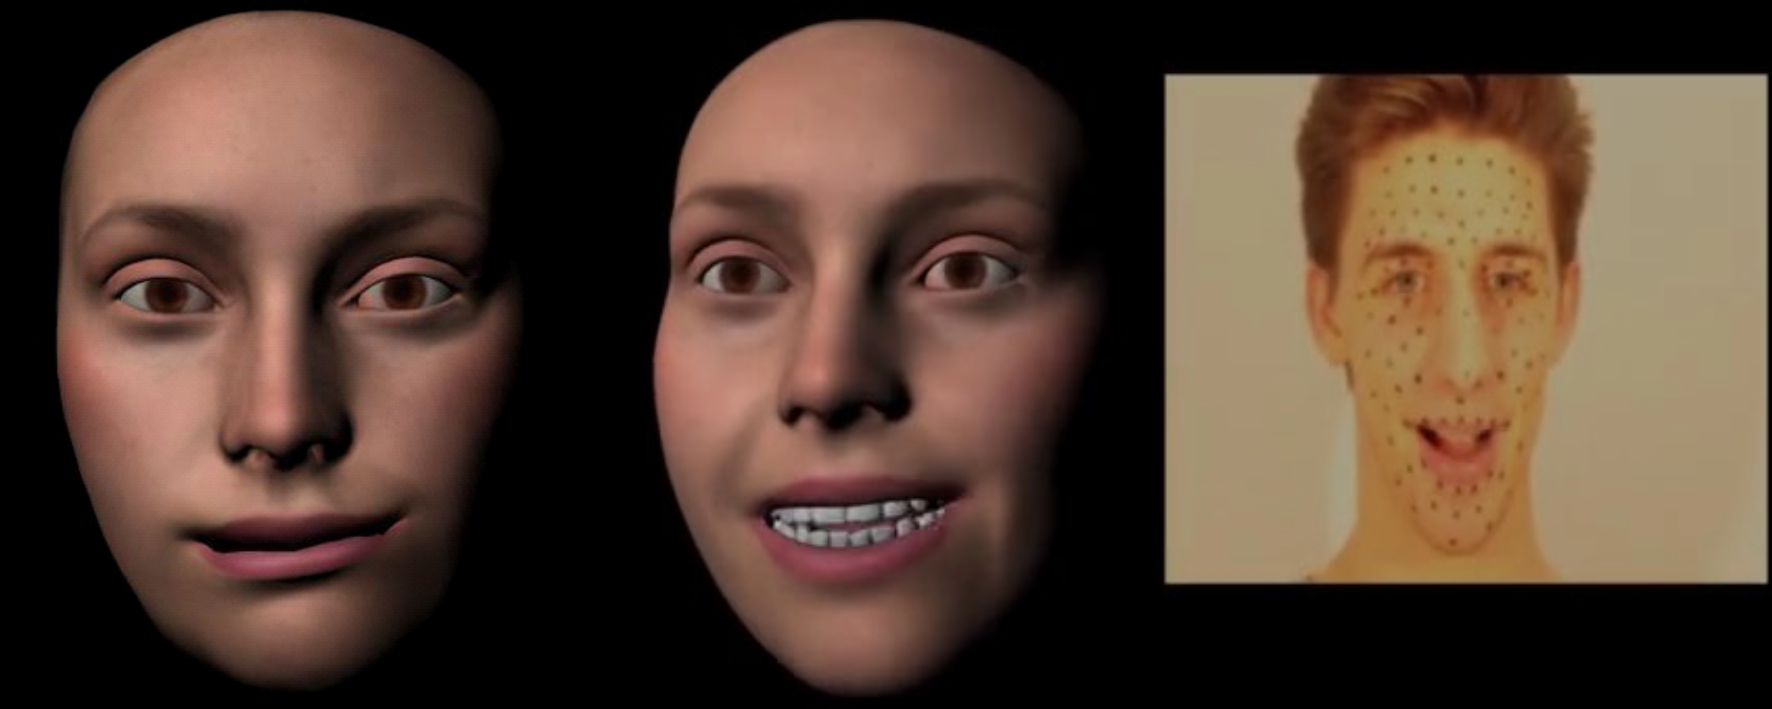
\includegraphics[width=\textwidth]{img/comp4s.png}
        \end{subfigure} \\
        \begin{subfigure}[b]{0.6\textwidth}
                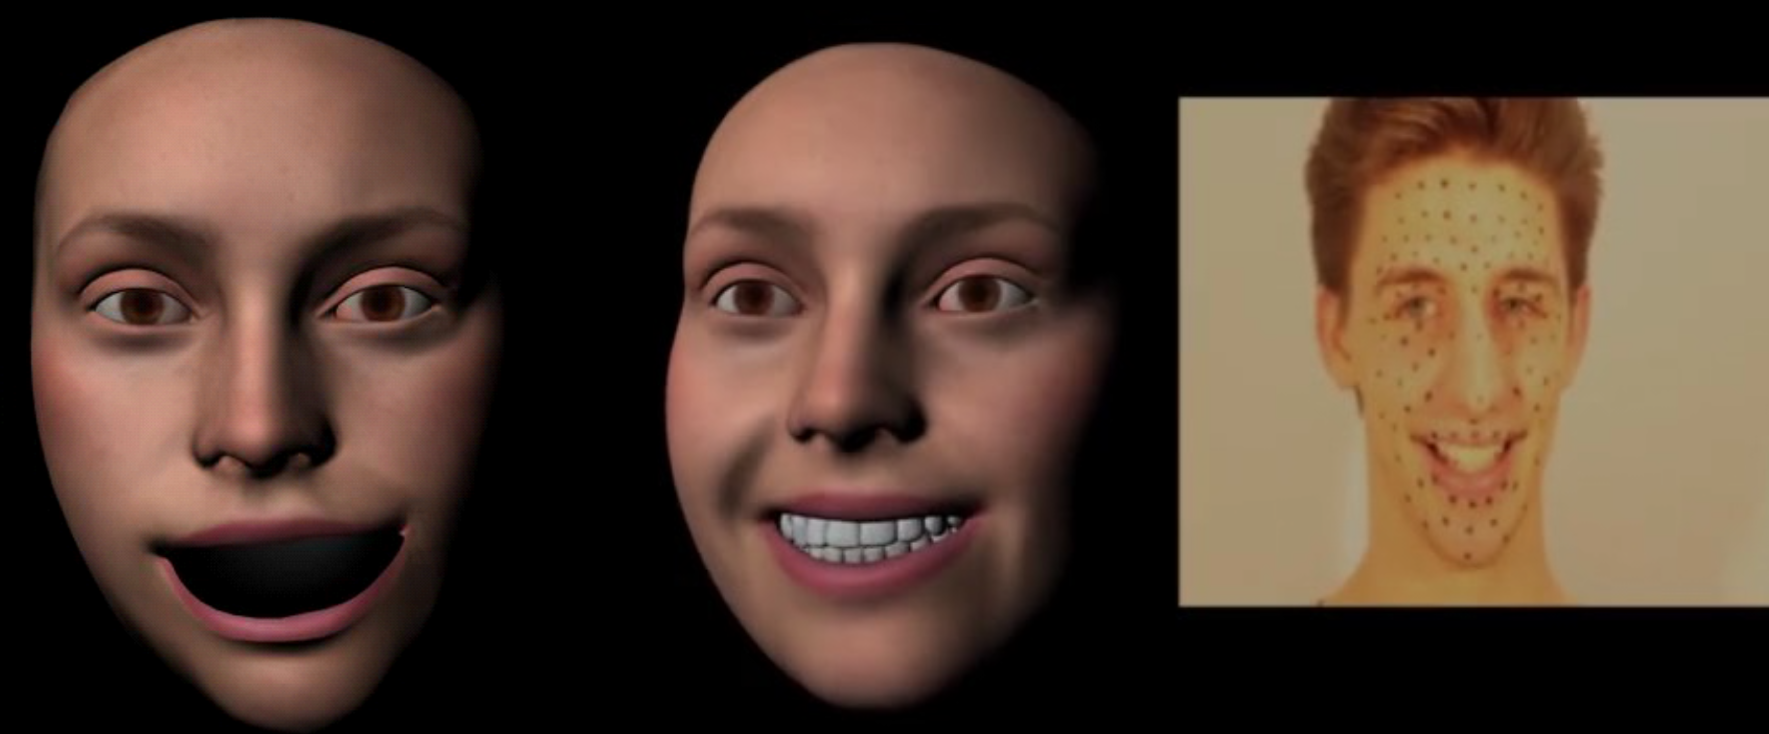
\includegraphics[width=\textwidth]{img/comp6s.png}
        \end{subfigure}
        \caption{The expressions on the left were produced using our original approach while the expressions in the middle use the weights that were calculated in the actor's domain. }\label{fig:resultcomp}
\end{figure}

We note that our final animation was not always able to capture the slight smiles that are noticeable in the recorded sequence. This may be explained by the poor match of neutral expressions. Specifically, all of the methods that we used rely on the transformation between the neutral faces. However, the actor's neutral expression is more positive (i.e. the corners of the lips are raised) than that of Emily, see Fig.~\ref{fig:neutrals}. This may be fixed by choosing a better matching neutral face from the actor's sequence, or by mimicking the actor's expression on Emily, and using that as her neutral. In our final results we use the second approach, and apply an additional small positive weight to the blendshapes that correspond to a smiling face, see Sec.~\ref{sec:implementation_details}.
\begin{figure}
        \centering
        \begin{subfigure}[b]{0.3\textwidth}
                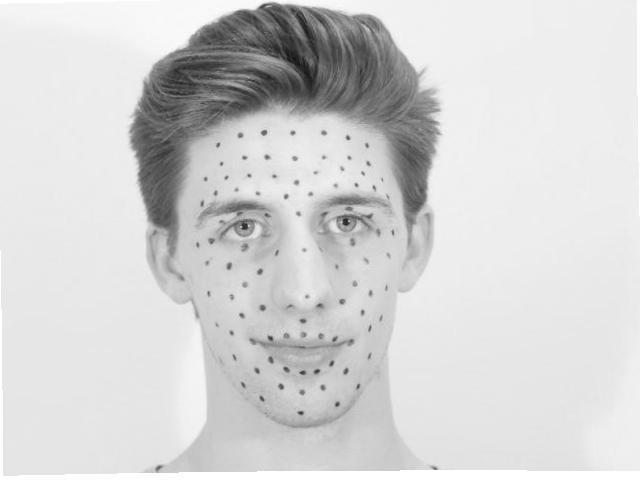
\includegraphics[width=\textwidth]{img/Richard2neutral}
        \end{subfigure}
        \begin{subfigure}[b]{0.4\textwidth}
                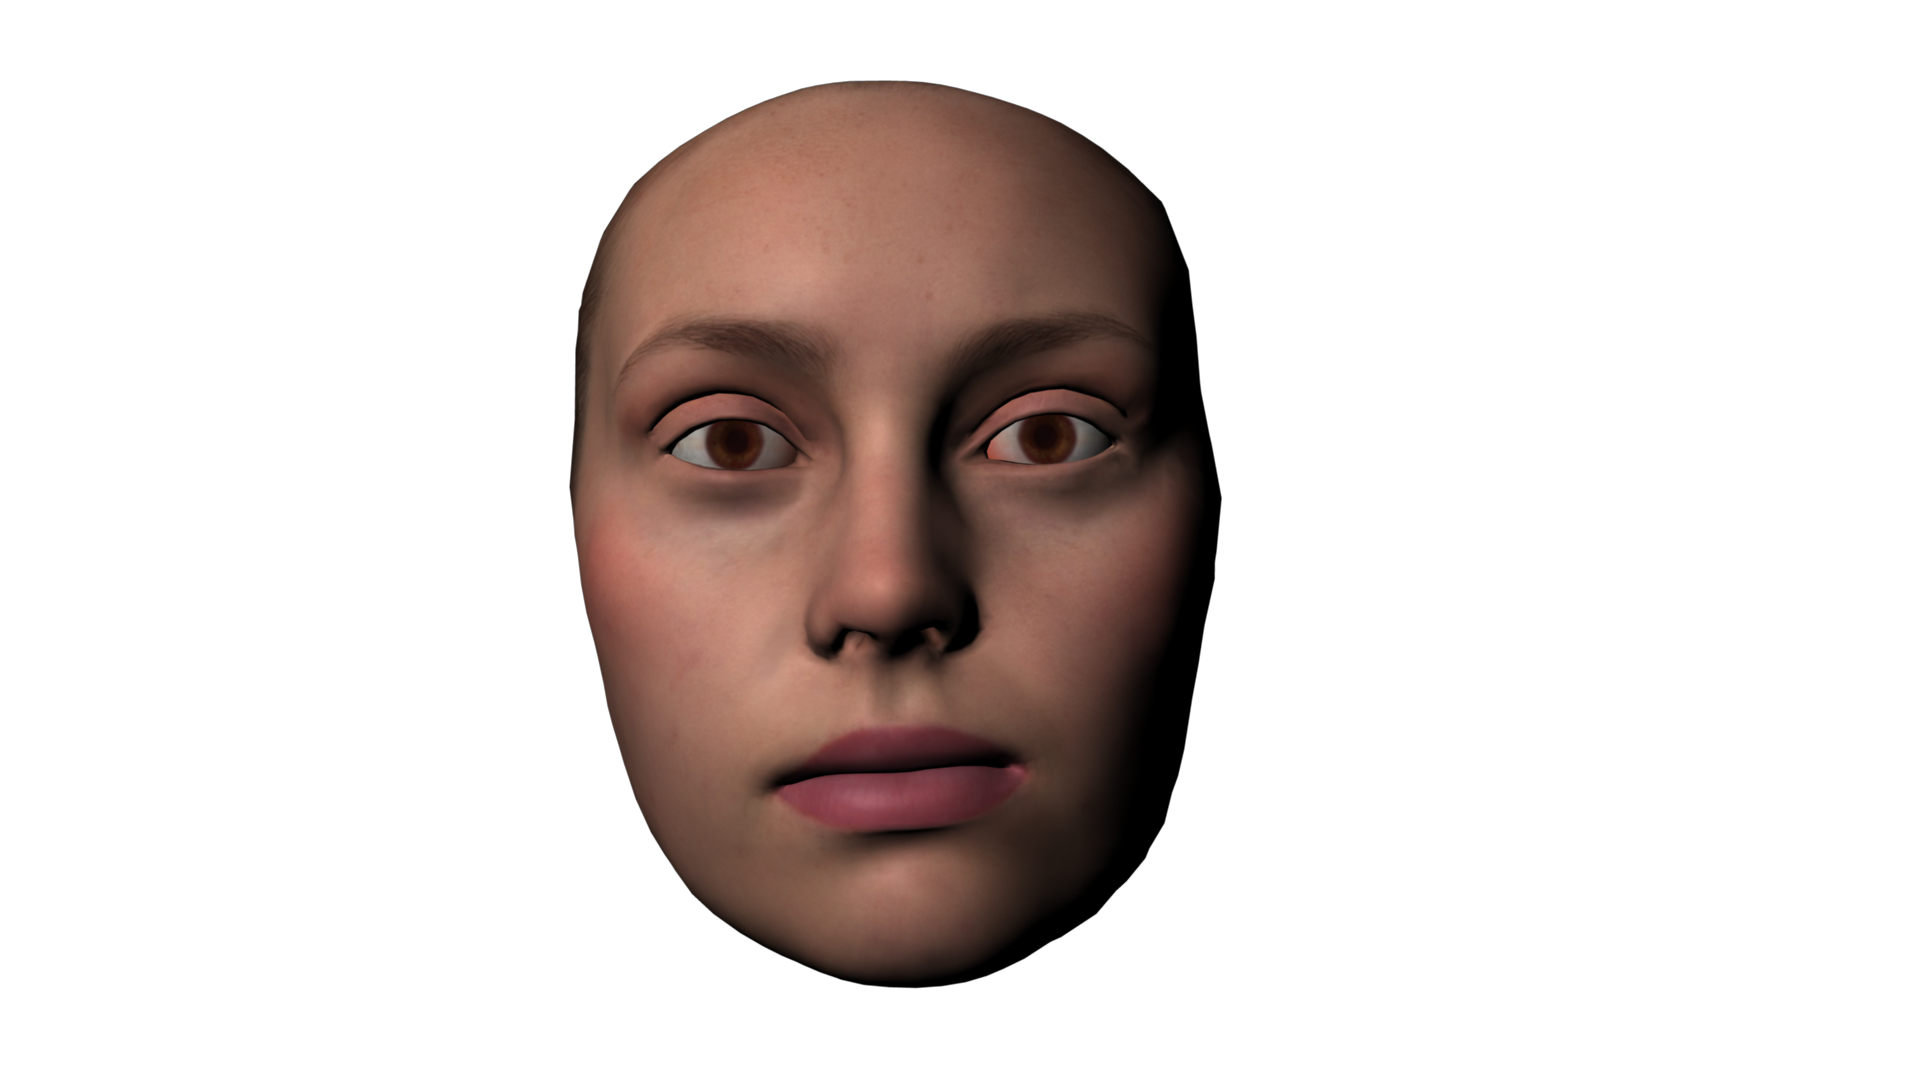
\includegraphics[width=\textwidth]{img/emily_neutral}
        \end{subfigure}
        \caption{The comparison of neutral expressions.}\label{fig:neutrals}
\end{figure}

\section{Skin Rendering}

Our objective in skin rendering is to generate a face that would be indistinguishable from a real one.
In our case, we have have taken a 3D scan of a subject and our aim is to improve the realism when rendering it.
For this task we will mainly look at the techniques presented by Hertzmann et al~\cite{Hertzmann2001} and Graham et al~\cite{Graham2013}.

\begin{algorithm}[htbp!] 
	\caption{Image Analogies}
	\label{alg:image_analogies}
	\KwData{$A$ unfiltered example, $A'$ filtered example, $B$ unfiltered source, $L$ number of levels, $k$ coherence parameter, $t$ neighbourhood size.}
	\KwResult{$B'$ filtered source image.}
	
	Compute Gaussian pyramids for $A$, $A'$ and $B$\;
	Compute features for $A$, $A'$ and $B$\;
	Build k-d tree for $\left\lbrace A, A' \right\rbrace$\;

	\For{$l$ = 0 to $L$}{
		\For{each pixel $q \in B'_l$}{
			$p_{app} =$ ANN search of $q$ neighbourhood from $\left\lbrace B, B' \right\rbrace$\;
			$r^* = \mbox{arg}\min\limits_{r \in N(q)} \left \| F_l(s(r) + q - r) - F_l(q) \right \|^2$\;
			$p_{coh} = s(r^*) + (q - r^*)$\;
			$d_{app} = \left \| F_l(p_{app}) - F_l(q) \right \|^2$\;
			$d_{coh} = \left \| F_l(p_{coh}) - F_l(q) \right \|^2$\;
			\eIf{$d_{coh} < d_{app}(1 + k2^{l-L})$}{
				$p = p_{coh}$
			}{
				$p = p_{app}$
			}
			$B'_l(q) = A'_l(p)$\;
			$s_l(q) = p$\;
		 }
	}
	\KwRet{$B'_L$}
\end{algorithm}

Before we begin, lets explain the Image Analogies framework~\cite{Hertzmann2001} in more detail.
Given three images $A$, $A'$ and $B$, where $A$ is an unfiltered example, $A'$ is a filtered example, and $B$ is an input image, the algorithm will generate an output image $B'$ such that $B'$ relates in the same way to $B$, as $A'$ does to $A$.
A k-d tree for an Approximate Nearest-Neighbour Search (ANN) is built using a feature vector from a neighbour pixel $p$ in $A$ and $A'$.
The closest match for a neighbourhood in pixel $q$ in $B$ and $B'$ is located in the tree.
A detailed description of the algorithm in pseudo code is shown in Algorithm~\ref{alg:image_analogies}, where $F$ is computed a weighted distance over the feature vectors using a Gaussian kernel and $s$ is a data structure such that $s(q) = p$.
Based on Ashikhmin's work, a match that is coherent to what has been already synthesized is computed.
These two candidates are weighted and the best one is chosen.
The whole process is carried in a multiresolution pyramid, as shown in Figure~\ref{fig:ia_diagram}, where $l$ indicates the current level, in essence this means that the neighbourhoods also include the previous level in the search.
We found three Image Analogies implementations available \cite{ImAnSingleThreadWeb, ImAnCudaWeb, ImAnHertzmannWeb}.
The first one is a simple single threaded implementation, the second one was done with CUDA, however the author's single threaded code produced overall better results.

\begin{figure}[htbp!]
\begin{minipage}[b]{.55\textwidth}
\centering
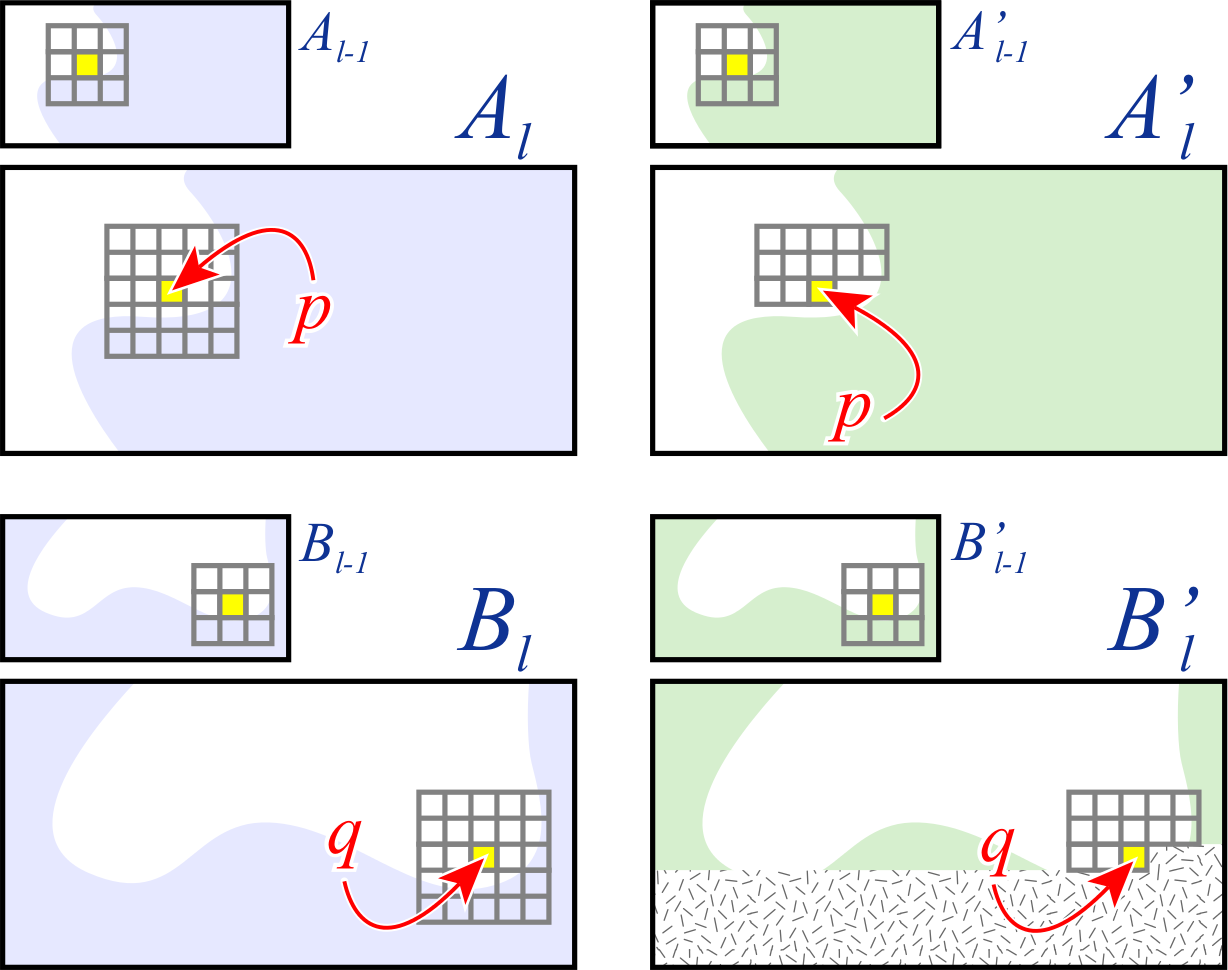
\includegraphics[width=\textwidth]{img/ia_diagram}
	\caption{ Neighbourhood matching for the Image Analogies framework, image taken from~\cite{Ashikhmin2001}.}
	\label{fig:ia_diagram}
\end{minipage}
\hfill
\begin{minipage}[b]{.4\textwidth}
\centering
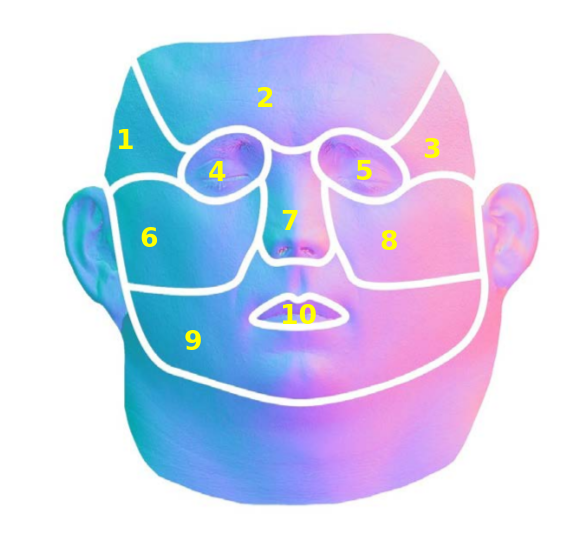
\includegraphics[width=\textwidth]{img/texture_synthesis_parts}
	\caption{ Texture segmentation in common coloured areas, image taken from~\cite{Graham2013}.}
	\label{fig:texture_synthesis_parts}	
\end{minipage}
\end{figure}

As a first step, we tried to reproduce the results for bump mapping quality increase by Graham et al~\cite{Graham2013}, results are shown in Figure~\ref{fig:bump_maps}.
The authors add an extra parameter $\alpha \in \left\lbrace 0, \ldots, 1 \right\rbrace$ to control Hertzmann's image synthesis process.
To be more precise, a match between $A$ and $\left\lbrace B,B' \right\rbrace$ will be weighted by $1 - \alpha$, and a match between $A'$ and $\left\lbrace B,B' \right\rbrace$ will be weighted by $\alpha$.
The logic behind this addition is to encourage more details of $A'$ to be included in $B'$.
The modifications required to include this addition begin by building two separated k-d trees for $A$ and $A'$, when choosing the best match both distances will be weighted as explained above and the smaller one will be chosen.
Also in the coherence match two searches will be done and weighted accordingly, and the final pixel will be chosen without further adjustments.

\begin{figure}[htbp!]
\centering
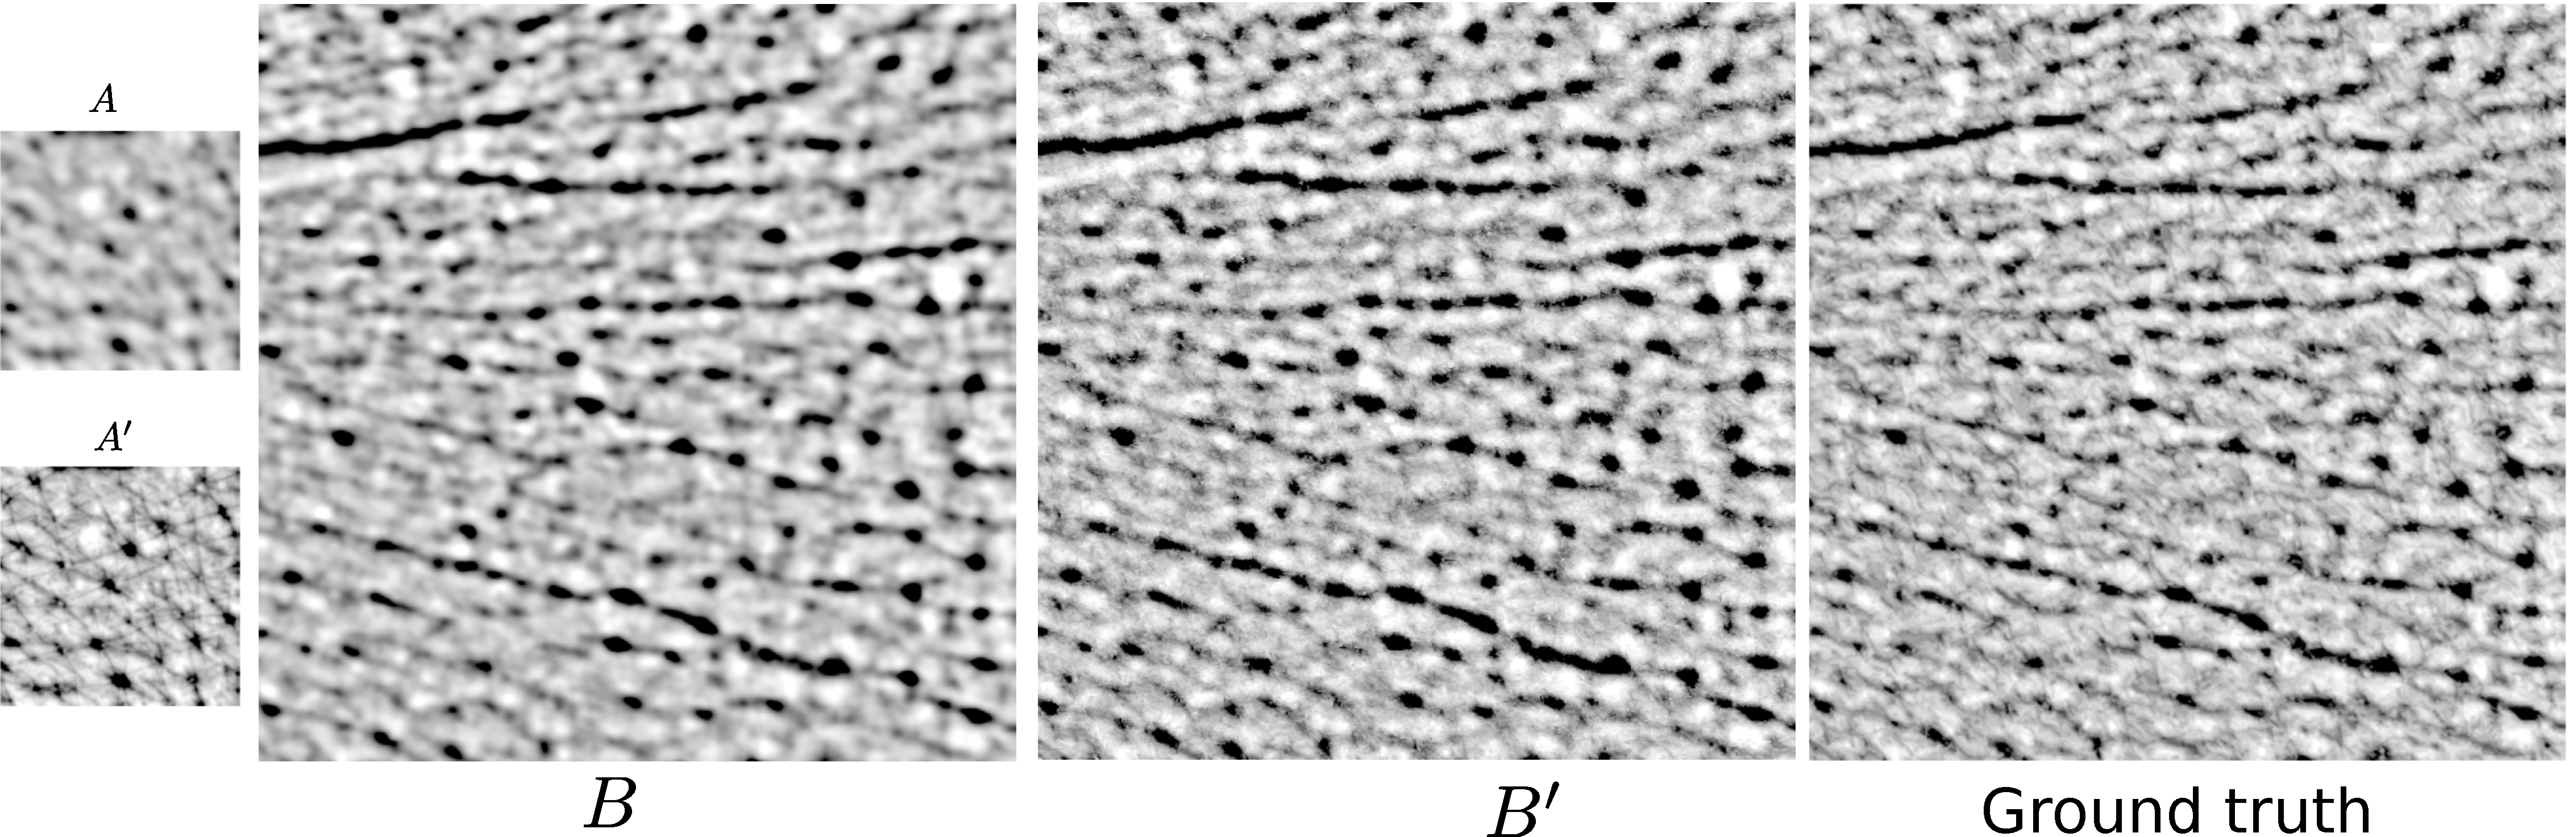
\includegraphics[width=\textwidth]{img/bump_maps}
	\caption{ Bum map deblurring, $A$, $A'$, $B$ and ground truth images images taken from~\cite{Graham2013}.}
	\label{fig:bump_maps}
\end{figure}

We also tried applying the Image Analogies filter to generate increased quality textures, which is in essence a deblurring filter.
The idea is to improve a low quality texture from a 3D scan using pictures of the texture taken at a closer range.
To achieve this we took a close up high quality sample $A'$, to generate $A$, the sample $A'$ was blurred using a Gaussian kernel until it look qualitative similar to the 3D scan texture $B$, with this three inputs we generated a picture $B'$ of higher quality.
Since faces have differentiated areas, this process was done separately for each relevant section in the face texture image, the generated patches are stitched together using linear interpolation.
The texture segmentation is shown in Figure~\ref{fig:texture_synthesis_parts} and results are shown in Figure~\ref{fig:texture_synthesis}.

\begin{figure}[htbp!]
\centering
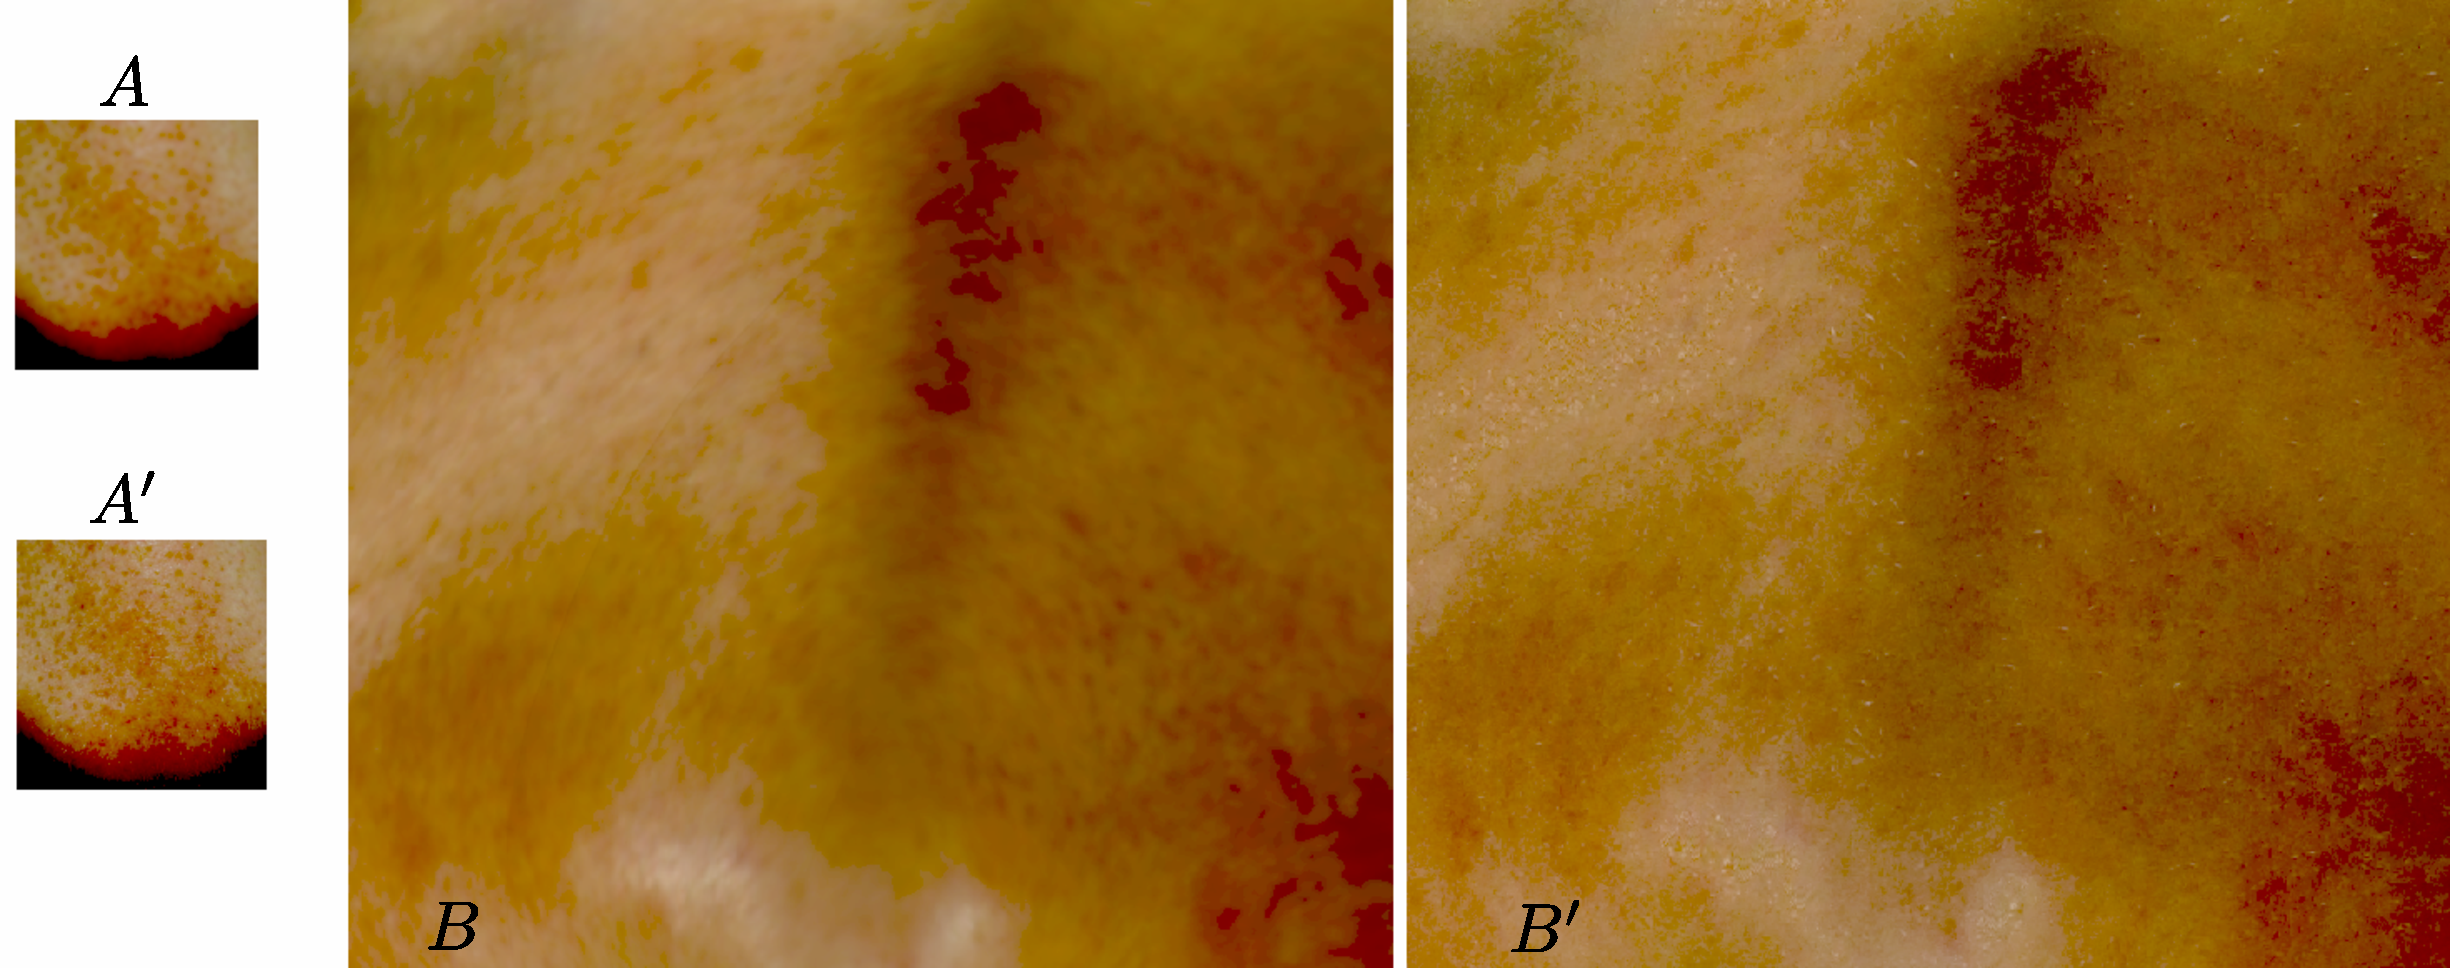
\includegraphics[width=\textwidth]{img/texture_synthesis}
	\caption{ Texture quality increase using image analogies, the texture is false-coloured to highlight the differences.}
	\label{fig:texture_synthesis}
\end{figure}

Another option for increasing the quality of the texture is to apply image super-resolution techniques, we used Jianchao et al~\cite{Jianchao2010} work for this purpose.
The idea is that by doubling the resolution of the original texture, yet avoiding blur by adding information from a dictionary of high resolution images, the final rendering quality of the face will increase.
Results for this approach are shown in Figure~\ref{fig:emily_super_resolution}.

\begin{figure}[htbp!]
\centering
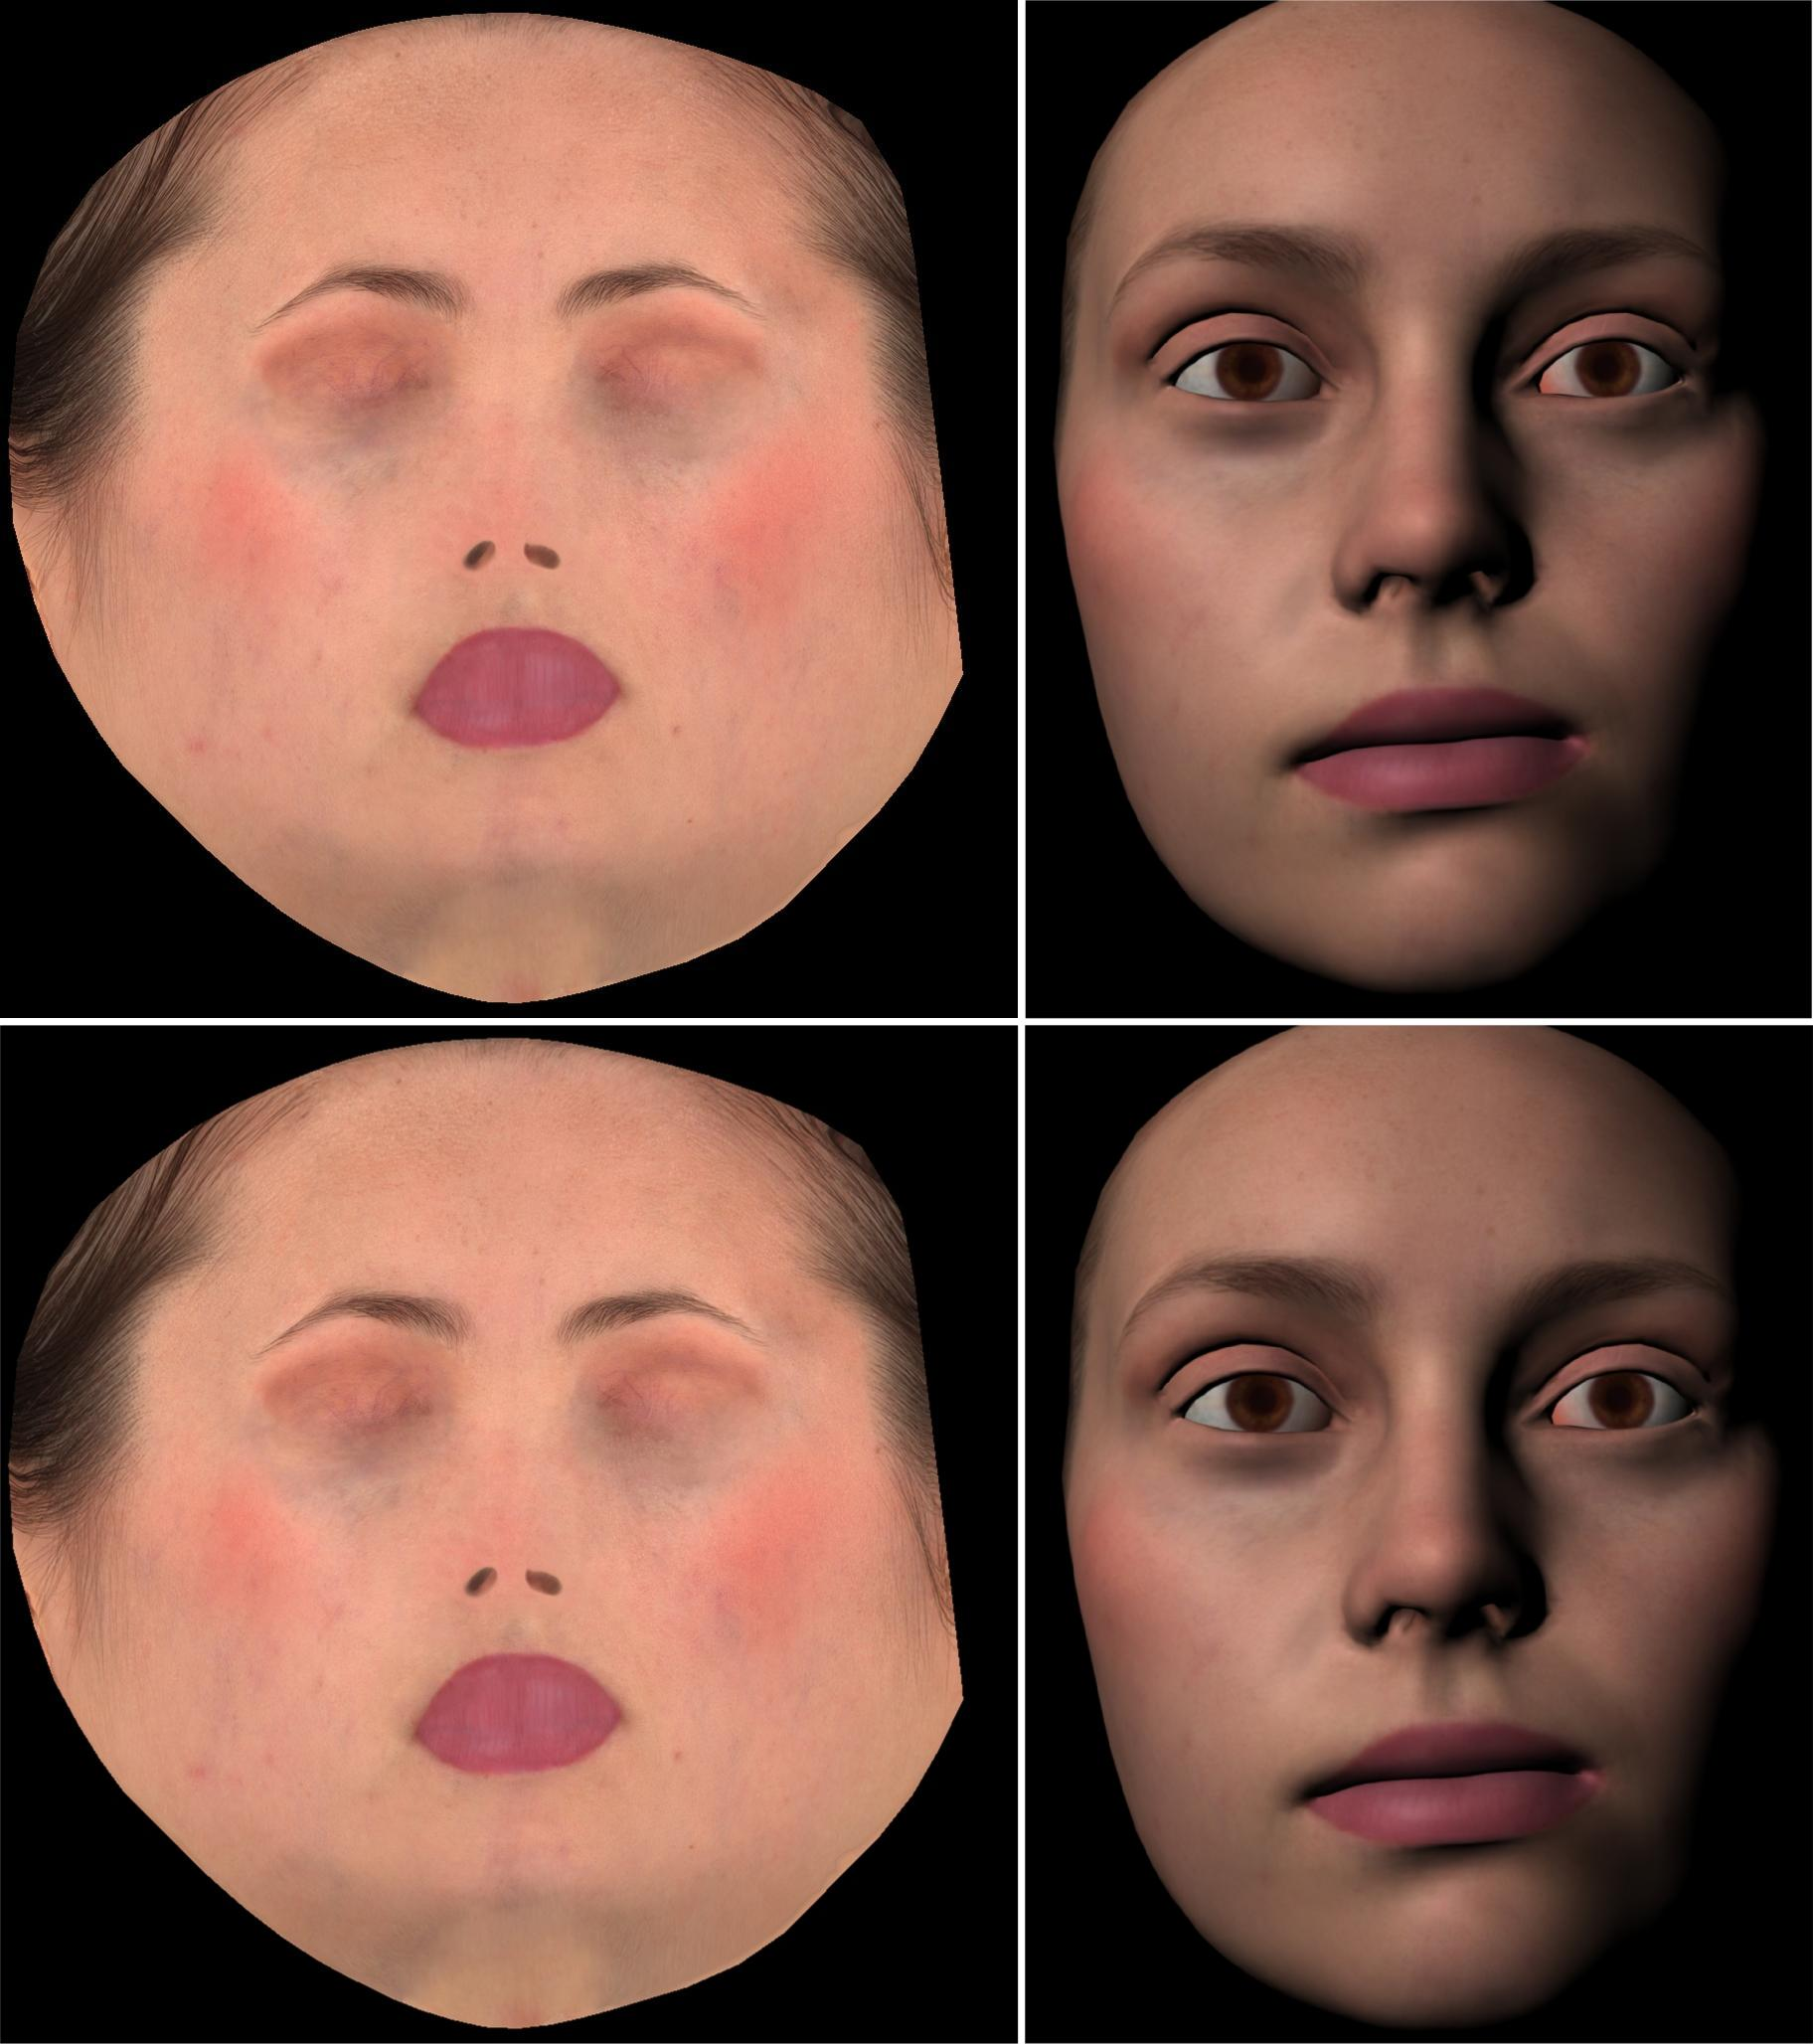
\includegraphics[width=\textwidth]{img/emily_super_resolution}
	\caption{ Super resolution example, left original texture, left-centre face rendered with original texture, right-centre super-resolution texture, right face rendered with super-resolution texture, original data from \cite{FaceWareWeb}.}
	\label{fig:emily_super_resolution}
\end{figure}

\begin{figure}
        \centering
        \begin{subfigure}[b]{0.48\textwidth}
                \includegraphics[width=\textwidth]{img/emily_close_original}
        \end{subfigure}
        \begin{subfigure}[b]{0.48\textwidth}
                \includegraphics[width=\textwidth]{img/emily_close_sr}
        \end{subfigure}
        \caption{Close up of texture super-resolution for Emily, (left) original texture, (right) synthesized texture with higher resolution.}
\end{figure}

Generating normals maps using Image Analogies is another interesting area, as it could provide an alternative to the costly standard capture methods.
For this we tried to generate a normal maps from albedo images and from bump maps generated from the previous 3D scan texture, results are shown in Figure~\ref{fig:normal_synthesis}. 
To create the bump maps, the textures were transformed to gray scale and a histogram equalization was applied.
In order to improve the quality of the bump maps, we also applied the Image Analogies filter to them using a known good bump map as a filtered example, results are shown in Figure~\ref{fig:bump_map_quality_increase}.

\begin{figure}[htbp!]
\centering
\includegraphics[width=\textwidth]{img/normal_generation}
	\caption{ Normal synthesis from albedo image.}
	\label{fig:normal_synthesis}
\end{figure}

\begin{figure}[htbp!]
\centering
\includegraphics[width=\textwidth]{img/bump_map_quality_increase}
	\caption{ Improving the quality of a bump map from a gray scale texture.}
	\label{fig:bump_map_quality_increase}
\end{figure}

The advantages of using a bump mapping are shown in Figure~\ref{fig:bump_mapping_richard}.
In this example, a render with the original texture is shown in Figure~\ref{fig:richard_original}.
The original RGB texture was converted to a gray scale image and applied directly as a bump map texture,
results are shown in Figure~\ref{fig:richard_disp_impr}, note how the addition of high frequency imperfections adds extra realism to the image.

\begin{figure}
        \centering
        \begin{subfigure}[t]{0.48\textwidth}
                \includegraphics[width=\textwidth]{img/richard_original}
                \caption{Render with the original texture.}
                \label{fig:richard_original}
        \end{subfigure}
        \begin{subfigure}[t]{0.48\textwidth}
                \includegraphics[width=\textwidth]{img/richard_disp_impr}
                \caption{Render with the original texture and bump mapping.}
                \label{fig:richard_disp_impr}
        \end{subfigure}
        \caption{The advantages of using a bump map..}
        \label{fig:bump_mapping_richard}
\end{figure}

\chapter{Implementation details}
\label{sec:implementation_details}

Talk about Maya plugins and any other implementation stuff worth talking about. 
..... Introduce the topic

We used the rigs for Maya that are provided for free by \cite{FaceWareRigsWeb}, the first thing to fix is to reset the paths for the textures in all the materials in the Hipershade window in \Maya.
The next step was to write plugin to load the weights from Matlab and set keyframes for each of them; to do this our plugin would create a new \Maya command that could be easily executed. 
The work flow for writing the code would be to first do the action in Maya manually if possible, see what MEL commands where executed, write them in the plugin and if possible rewrite them as pure C++ code instead of MEL commands.
The file format for the weights is one weight per line in frame order, as shown in Figure~\ref{fig:file_format}, where $N$ is the number of weights and $F$ is the number of frames.
Once we have the weights loaded, the connections between the blenshape object weights and its outputs have to be broken, this is done in order to be able to set the keyframes, otherwise the setKeyframe function would not work, an extract of the code is shown in Listing~\ref{lst:set_weights}.
Additionally, we program our code to comply with \Maya undo command policy, which means using the \emph{DagModifier} class or manually undoing the actions, however in the final stages of our implementation it was faster to reload the scene that to undo de command.

\begin{figure}[htbp!]
\centering
\includegraphics[width=0.1\textwidth]{img/file_format}
	\caption{File format for weights import and export.}
	\label{fig:file_format}
\end{figure}

\begin{lstlisting}[caption = Breaking the weights connections and setting keyframes., label = lst:set_weights, frame=single, float]

// Break connections.
for (unsigned int i = 0; i < (unsigned int)(numWeights); i++){
		cmd = "disconnectAttr shapesBS_";
		cmd = cmd + names[i];
		cmd = cmd + ".output shapesBS.";
		cmd = cmd + names[i];
		dgMod.commandToExecute(cmd);
}

// Set key frames
for (unsigned int j = 0; j < weights.at(i).size(); j++){
		cmd = "setAttr shapesBS.weight[";
		cmd = cmd + j;
		cmd = cmd + "] ";
		cmd = cmd + weights.at(i).at(j);
		dgMod.commandToExecute(cmd);
		
		cmd = "setKeyframe { \"shapesBS.w[";
		cmd = cmd + j;
		cmd = cmd + "]\" }";
		dgMod.commandToExecute(cmd);
	}
}
\end{lstlisting}

Once the weights were added, we noticed that the teeth and tongue of the Emily rig would not move.
Both meshes were actually regulated by the position of a control object in the scene, so the solution was to translate the object by a factor of the mean of all the weights involved in the mouth control, as shown in Listing~\ref{lst:teeth_tonge_control}.
The lower teeth and tongue would be left hanging mid air if the blendshapes that control the mouth opening were activated together; this problem was fixed by lowering the position of both meshes.

\begin{lstlisting}[caption = Teeth and tongue control based on relevant weights., label = lst:teeth_tonge_control, frame=single, float]

cmd = "setAttr con_jaw_c.translateY ";
cmd += -3.2 * (weights.at(i).at(58) + weights.at(i).at(55)) + 1;
dgMod.commandToExecute(cmd);
cmd = "setKeyframe  \"con_jaw_c.translateY\"";
dgMod.commandToExecute(cmd);
\end{lstlisting}

The next step was to include head rotation and translation back into the animation.
In order to achieve this, we saved the inverse rotation from the Procustes analisys that was performed on Section~\ref{sec:stabilising_head_movement}, into a file with the same format as shown in Figure~\ref{fig:file_format}.
We then read the data into \Maya and applied the transformation for each frame; for the translation we did a equivalent procedure with a translation file.
Note that Matlab matrices are column-wise while \Maya matrices are row-wise, so we read them taking into account this consideration.
The matrix multiplication order also plays in important role here, as shown in Equation~\ref{eq:rotation_translation_inv}, to achieve the correct result we need to undo the translation first and rotate the result.

\begin{equation}
\mathbf{x}_{new} = R\mathbf{x} + \mathbf{t} ~ \rightarrow  R^{-1}(\mathbf{x}_{new} - \mathbf{t}) = \mathbf{x},
\label{eq:rotation_translation_inv}
\end{equation}

where $\mathbf{x}$ is the original point, $\mathbf{x}_{new}$ is the transformed point, $R$ is the rotation matrix and $\mathbf{t}$ is a translation vector.
We implemented this transformation in \Maya using the ``xform -m" command, so we first apply the translation and then apply the rotation with an extra parameter ``-r" so that both matrices get multiplied in the desired order.

Having eye movement is quite important to achieve realism in the animation, for this purpose we tracked the pupils' world positions in the input frame sequence.
These positions were saved into separate files for each eye using the format shown in Figure~\ref{fig:file_format}.
The positions were loaded into \Maya and the eye control object was translated using the offsets with respect to the first frame, which was assumed to be looking straight.
With this first approach each eye can move independently which leads to unsatisfactory results, an initial solution to this problem was to move both eyes using the mean offset for each frame.
Nevertheless, this would introduce considerable error when one of the eyes winks, as the tracking becomes completely unreliable for the winking eye which in turn drags the other eye.
Our solution involves interpolating between the two offsets using variable factors.
The idea is to have both eyes moving together, start ignoring the offset for an eye if it goes off, while sustaining smooth movements.
The final offset $d_f$ will be computed as $d_f = \alpha d_l + \beta d_r$, where $\alpha$ and $\beta$ are the interpolation factors, $d_l$ and $d_r$ are the offsets for the left and right eye, respectively.
Figure~\ref{fig:eyes_interpolation} shows the $\alpha_x$ values along the $x$ direction, where $t$ is the change threshold and $l$ is the maximum offset limit.
Initially $\alpha_x$ is $0.5$, however if the offset goes beyond a threshold $t$, $\alpha$ will decrease linearly until it reaches the limit $l$.
The same criteria will be applied in the $y$ direction, and the value for that eye will be $\alpha = \min \left\lbrace \alpha_x, \alpha_y \right\rbrace$.
The $\beta$ factor will be computed as $\beta = 1 - \alpha$, however, if the right eye is the one surpassing the threshold $t$, then the whole process will be reversed. 
Additionally, if both eyes surpass the threshold $t$, $\alpha$ and $\beta$ will be $0.5$, this will allow the eyes to move together beyond the threshold if needed.

\begin{figure}[htbp!]
\centering
\includegraphics[width=0.8\textwidth]{img/eyes_interpolation}
	\caption{Offset interpolation for eye movements in \Maya.}
	\label{fig:eyes_interpolation}
\end{figure}

Incorporating blinks was another important step towards attaining a more realistic animation.
Since the eyelids were not tracked in the recording session, the only option was to manually set the blinking times in \Maya.
To faithfully reproduce the blinking in the data the following information was manually added:
\begin{itemize}
\item Frame number marking when the eye:
	\begin{itemize}
	\item started closing;
	\item closed completely;
	\item started opening again;
	\item was fully open again;
	\end{itemize}
\item The blink magnitude (eyes fully close, squinting, etc);
\item The blink type (both eyes closed, only one eye).
\end{itemize}

%-----------------------------------------------------------------------
\chapter{Results}
In this chapter we shall introduce our final results, highlight the strengths and weaknesses, and compare the results we have produced throughout the course of this project.

In general, our final animation well resembles the motion of the actor, see Fig.~\ref{fig:results1}. The animation runs at $60$ frames per second, it is smooth and expressive, see the video in the supplementary material. The animation respects the intrinsic differences between the actor and Emily, i.e. the animated expressions are not exact replicas of the actor's expressions; instead they are Emily versions of the actor's expressions. The final result was enhanced by manually activating the blendshapes that control blinks and winks throughout the motion sequence, see Fig.~\ref{fig:results2a}. Moreover, the head motion that we removed before solving for blendshape weights (see Sec.~\ref{sec:stabilising_head_movement}), was reintroduced to make the animation appear more dynamic, see Fig.~\ref{fig:results3}.

\begin{figure}
        \centering
        \begin{subfigure}[t]{0.43\textwidth}
                \includegraphics[width=\textwidth]{img/results/Emily_Maya_clean_video_300}
        \end{subfigure}
        \begin{subfigure}[t]{0.43\textwidth}
                \includegraphics[width=\textwidth]{img/results/Emily_Maya_clean_video_1187}
        \end{subfigure}\\
        \begin{subfigure}[t]{0.43\textwidth}
                \includegraphics[width=\textwidth]{img/results/Emily_Maya_clean_video_1544}
        \end{subfigure}
        \begin{subfigure}[t]{0.43\textwidth}
                \includegraphics[width=\textwidth]{img/results/Emily_Maya_clean_video_2135}
        \end{subfigure}
        \caption{The final animation well resembles the captured sequence.}
        \label{fig:results1}
\end{figure}
\begin{figure}
        \centering
        \begin{subfigure}[t]{0.43\textwidth}
                \includegraphics[width=\textwidth]{img/results/Emily_Maya_clean_video_775}
                \caption{Manually added blinks.}\label{fig:results2a}
        \end{subfigure}
        \begin{subfigure}[t]{0.43\textwidth}
                \includegraphics[width=\textwidth]{img/results/Emily_Maya_clean_video_2941}
                \caption{Reintroduced the head rotation.}
        \end{subfigure}
        \caption{Improvements to the blendshape model.}\label{fig:results2b}
        \label{fig:results2}
\end{figure}

The final animation has a number of flaws. First, since only a sparse set of points is used to find the blendshape weights, some motion remains poorly captured; Fig.~\ref{fig:results3a} presents such a situation. Here the sparse points alone are unable to define the downward positioning of the mouth; the markers around the mouth form a ellipse which is then replicated by Emily without taking into consideration the fact that the actor's mouth is shut. Another issue is visible in Fig.~\ref{fig:results3b}; here the spherical structure that represents the inside of the mouth is penetrating Emily's cheek. Unfortunately, we have no control over the motion of this inner structure, and it cannot be hidden since it is connected to the mesh of the face. Our approach to this problem involves limiting the upper bound on the weights to ensure that the combination of blendshapes that cause this problem does not occur; by trial and error we were able to eliminate most of the problematic mixtures of shapes.

\begin{figure}
        \centering
        \begin{subfigure}[t]{0.43\textwidth}
                \includegraphics[width=\textwidth]{img/results/Emily_Maya_clean_video_2578}
        \caption{Sparse data does not describe the motion fully.}\label{fig:results3a}
        \end{subfigure}
        \begin{subfigure}[t]{0.43\textwidth}
                \includegraphics[width=\textwidth]{img/results/Emily_Maya_clean_video_2631}
		\caption{The mesh inside the mouth is allowed to penetrate itself.}\label{fig:results3b}        
        \end{subfigure}
        \caption{Shortcomings of the current model.}
        \label{fig:results3}
\end{figure}



%-----------------------------------------------------------------------
\chapter{Conclusions and Future Work}
\section{Conclusions}
The objective of our project was to produce a prototype pipeline that takes captured facial performance as input, and creates an animation of a three-dimensional model of a human face. 

The quality of an animation may be evaluated in a number of different ways. In our final animated sequence Emily is able to closely mimic the motion of the actor while retaining individuality imposed by the structure and features of Emily's face. The realism of our animations improved with time; the first animation has no eyes or mouth, and it exhibits unusual behaviours. On the contrary, the final animation includes motion of the eyes and the teeth, as well as more plausible overall performance, thus it looks significantly more appealing. Though more realistic than a hand-drawn character or an industrial robot, our results lack the naturalness of human motion. We believe that our results belong in the uncanny valley of the familiarity versus human likeness diagram, see Fig.~\ref{fig:UV}. The theory of the uncanny valley suggests that human-like appearance and behaviour is perceived as repulsive as the resemblance increases~\cite{UV}.
\begin{figure}[htbp!]
\centering
\includegraphics[width=0.8\textwidth]{img/UV}
	\caption{Our animations in the context of the uncanny valley.}
	\label{fig:UV}
\end{figure}

% Rendering was improved when doing super-resolution on the textures.
% Improvement only noticeable at close ups
% Improvement was only marginal


\section{Future Work}

There are a number of different techniques that could be used to construct blendshapes in the actor's domain. Deng et al. proposed designing the blendshapes by hand~\cite{Deng:2006}. In particular, the authors choose a number of characteristic frames in the motion capture sequence, and manually design a set of shapes that perceptually match the expressions observed in these frames. They then form correspondences between the PCA coefficients of motion capture frames and the weights of the blendshapes. Finally, Radial Basis Functions are used to map the new frames in the sequence onto the three-dimensional model to produce the animation. Another option would be to use a muscle actuation basis, proposed by Choe and Ko~\cite{Choe:2005}. The design of a muscle actuation basis is based on the human facial anatomy, and is driven by the actuation of different facial muscles. Our main reservation about these approach is the extensive manual effort required to design the set of initial correspondences between the chosen frames and the three-dimensional mesh.

The accuracy of the model may be improved by taking extra care when matching the sparse points on Emily and the actor. One possible approach involves drawing a number of stable points on Emily and the actor and finding the mapping that transforms sparse Emily points to the actor's domain. Then a large number of additional points are drawn on Emily, and the same transformation is used to transform these points to the actor's domain. These points are then used to identify the ideal location of the markers on the actor's face. Moreover, a 3D printed mask may be used to ensure high accuracy when placing the markers. % THIS PARAGRAPH DOESN'T SOUND RIGHT. I FORGOT WHAT I WAS TRYING TO DAY.

The main weakness of the current method is the amount of manual work that needs to be done before the animation takes its final shape. 
% We could track eyelids and add blinks automatically.


% Including wrinkles.

% Talk about adding BSSRDF to the skin rendering
% Adding normal maps for more detail -> capture studio with light dome






\newpage
\bibliographystyle{eg-alpha}
\bibliography{baththesis}

\end{document}